\chapter{Validation of \acs{BDI} \acsp{MAS} via Simulation}
\label{chap:simulation}

Part~\ref{part:background} and Part~\ref{part:nextgen} discussed how \ac{BDI} agents can be designed and engineered
as autonomous entities that react to their environment, reason about their goals, and act accordingly.
%
It also discussed how \jakta{} embeds these abstractions within a mainstream, statically-typed language.
%
Having a practical way to \emph{build} \ac{BDI}-based \acp{MAS}, however, is only part of the problem:
these systems must also be \emph{evaluated} before deployment.

When engineering a \ac{BDI}-based \ac{MAS},
and especially when the target system is distributed,
unit-testing may be unable to provide a satisfactory coverage of all required conditions,
particularly concerning responses to changes in the environment.
%
Moreover, testing the system on a single device is typically insufficient,
and verification on a real-world setup is, on the other side,
unfeasible due to time and cost:
\emph{simulation} is a necessary tool
to evaluate the behaviour of non-trivial situated \acp{MAS}. 
%

In the context of \acp{MAS},
simulations are typically supported by \ac{MABS} frameworks~\cite{DrogoulVM02,BandiniMV09},
of which many have been proposed in the literature,
for instance, NetLogo~\cite{Sklar07}, Mason\cite{LukeCPSB05}, or RePast~\cite{NorthCOTMBS13}.
%
However, these toolkits are designed to expose their custom notion of agent,
which is typically much simpler than the nuanced design behind \ac{BDI} agents:
adopting a classic \ac{MABS} framework
to simulate a \ac{BDI} \ac{MAS}
incurs into a significant cost induced by the abstraction gap
separating the two technologies.
%
Both \ac{MABS} and \ac{AOP} offer their \ac{MAS} specification language,
to let developers model and encode their systems in an agent-oriented program.
%%
However,
we observe that \ac{MABS} technologies offer low-level, and simulation-specific, abstractions
which do not really capture agents' cognitive features or capabilities.
%%
At the same time,
\ac{AOP} technologies only offer minimal support for simulating articulated scenarios
in a reproducible and scalable way.
%
One critical consequence of this technological gap is that \acp{MAS} are rarely both simulated and deployed,
because the program must be implemented twice:
once, using \ac{BDI} abstractions, for the production system;
and once, using \ac{MABS} abstractions, for its simulation.
%
Moreover, due to the misalignment of the syntax,
there is no guarantee that the two implementations do exactly the same job;
indeed, they often do not,
as the simulated version only captures a fraction of the complexity of the production one since
producing two equivalent versions would be costly,
as the simulated version would need a re-implementation of the cognitive features of the agents.

Even if developers decide to implement these two different versions of the same program but for different purposes,
maintenance becomes a burden.
%
Changes into the \ac{BDI} code base are not automatically reflected into the \ac{MABS} code base,
requiring continuous re-alignment to prevent divergent behaviours.
%
The outcome of this misalignment is that,
often,
simulations performed on an initial version of the system get abandoned as the system evolves,
and, therefore, the system gets progressively less and less verified.

The aim of this analysis is allowing a single \ac{BDI} system definition to 
run on a simulated scenario, to validate the correctness of its emerging behaviour, 
and then execute it in the production with minimal or no changes.

The idea of testing the behaviour of a \ac{MAS} through simulation
is not new~\cite{uhrmacher_simulation_2002}.
%
However, 
there are not many tools that effectively allow one
\emph{
    ``to execute agents as they are and to switch arbitrarily between execution in the real environment and the virtual test environment''
}\cite{uhrmacher_simulation_2002}.

%% Introduce following chapters here, and explain how they are related to the problem of simulation and validation of BDI MAS.

\chapter[Testing BDI-based MAS using DES]{Testing BDI-based Multi-Agent Systems using Discrete Event Simulation}
\label{chap:bdi-simulation}

Modern software systems are increasingly complex,
and novel programming paradigms are emerging
to tackle application domains such as
\acp{STS}~\cite{sociotech}, \acp{CPS}~\cite{cps}, or \acp{PS}~\cite{pervasive},
where people interact with many computational entities situated in a physical environment
that feature automation, autonomy, and intelligence.
%
In these contexts,
\acp{MAS} have been widely adopted to tame complexity~\cite{Xie2017},
as they model software as a collection of interacting autonomous entities.

Depending on whether \acp{MAS} were exploited to \emph{study} systems' complexity,
or to \emph{tame} it,
many solutions have been proposed to either
use \ac{MAS} abstractions to \emph{simulate} system behaviour~\cite{BandiniMV09}
or for designing and \emph{deploying} real-world systems~\cite{CalegariCMO21}.

The difference is subtle but crucial.
%
When simulated,
agents operate in a virtual sandbox environment
designed to imitate the dynamics of the target real-world deployment
in which perceptions (e.g., data from sensors, the flow of time)
and actions (e.g., agents' movements in the environment)
are controlled by the simulator,
and can be reproduced deterministically.
%
When deployed, agents are attached to specific hardware and software runtimes,
communicate through networks, and are tied to the flow of real time.
%
Agents could either run in virtual environments as concurrent
(and often distributed) processes
interacting with shared resources
(e.g., files, databases, network sockets)
hence perceiving the state of such resources in real time and acting on them.
In some cases, agents may even be embodied in physical entities
(e.g., robots, drones, embedded devices)
hence perceiving and acting through physical sensors and actuators.
%
Any of these elements may introduce non-determinism and unpredictability in the system,
to which the \ac{MAS} must be ready to react.

Accordingly, in this paper, when referring to \emph{real-world deployment},
we intend software agents running on their final ``production'' platform
rather than within a simulation,
regardless of whether they are situated in a physical environment or not.
With \emph{real world} we therefore mean the target execution context for which the agents
are designed and implemented.

Aside from being useful in in-silico studies,
\emph{simulation} may also aid the \emph{development} and \emph{validation}~\cite{uhrmacher_simulation_2002}
of \acp{MAS} intended for real-world deployment.
%
In fact, simulation enables developers to test the behaviour of agents
and their dynamics in complex environments ahead of deployment,
while postponing and (ideally) reducing costs and efforts, while mitigating risks, associated with real-world execution.
%
%For instance,
%distributed settings,
%corner cases,
%or emergent phenomena could be observed and tested as early as possible,
%
The price for
having the possibility to test a \ac{MAS} specification in a simulated environment
%such flexibility, however,
is paid in additional development effort.
First and foremost, developers must model the \emph{target} deployment context as a simulation environment.
%
Moreover, developers must develop the behavior of the agents within the simulation framework, which may differ from the one used for real-world deployment, making sure
to maintain alignment between the two versions of the \ac{MAS} codebase.

While the first challenge is unavoidable for any kind of simulation,
we argue that the second one could be mitigated in case that the same \ac{MAS} specification can execute \emph{with no changes}
on both real hardware and a simulator of choice.

The situation is particularly challenging when dealing with \acp{MAS} featuring cognitive models of agency,
such as the \ac{BDI} model~\cite{RaoG95}.
%
\ac{BDI} agents have been proposed for complex scenarios, including
healthcare~\cite{CroattiMRGAA19},
multi-\acs{UAV} coordination~\cite{SilvestreLDBHB23},
social simulations~\cite{AdamGaudou2016},
and
cyber-security~\cite{NunesSF17}.
%
% However,
% creating high-fidelity simulations of \acp{BDI} systems is particularly challenging,
% due to the current state of the art in \ac{BDI} technologies.
%
% As we further argue in \Cref{sec:background},
% tools supporting \acp{MABS} do not directly support the \ac{BDI} model,
% while tools for \ac{BDI} programming do not directly support simulation%
% ---being designed for real-world deployment.
%
The abstraction gap between the \ac{BDI} programming model and most simulators~\cite{singh_integrating_2016},
along with the minimal support of \ac{BDI} technologies
for producing \emph{reproducible} simulations of articulated scenarios
lead developers to resort to one of the following approaches:
%
\begin{enumerate}
    \item extension of the \ac{BDI} platform with a dedicated simulation engine,
    which requires additional development effort;
    \item construction and maintenance of two parallel codebases
    (one for simulation and one for the actual system),
    leading to consistency issues;
    or
    \item integration of the \ac{BDI} platform with a general-purpose simulation engine,
    typically by synchronising their execution through some form of middleware~\cite{singh_integrating_2016}.
\end{enumerate}

All such approaches come with their own drawbacks,
and,
above all,
they are symptomatic of the lack of a general solution.
%
In fact,
while the effort of modelling the environment is unavoidable for any simulation
-- and challenging per se~\cite{simchallenges} --,
porting agents' behaviour back and forth between simulation and real systems
should be as simple as possible,
ideally requiring no changes to the code.

\paragraph{Problem Statement}
% \samu{forse mancano le ipotesi, può aver senso la formulazione di research questions esplicite?}
% \gcnote{le ipotesi di ricerca, quali sono secondo te?
% io ci avevo pensato e facevo fatica a distillare frasi concise che non fossero già nel sottotesto del resto dell’introduzione}
% \danilo{``ipotesi'' intese come research questions?}
In our view,
the state of the practice of \ac{BDI} systems engineering
lacks a general-purpose, practical solution for testing \ac{BDI} systems using simulation,
before deployment.
%
Put differently,
switching between simulation and real-world deployment is currently cumbersome and impractical.
%
Ideally,
starting from the same codebase expressing a \ac{BDI} system specification,
developers should be able to test it in a simulated environment,
or run it on real hardware,
with no changes to the codebase,
while expecting the system to behave consistently in both scenarios.

The problem may seem merely technical,
but indeed reaching this goal requires redesigning how \ac{BDI} specifications are written and interpreted.
%
They should abstract away the implementation details of their execution,
while multiple execution engines should support both simulations and real-world deployments.
%
In the particular case of simulations,
the environment as well should be programmable,
other than only agents.

% \samu{il paragrafo che segue non mi è per niente chiaro, e mi sembrano due concetti scollegati messi insieme}
% From an engineering standpoint,
% a critical challenge here is
% to avoid reimplementing multiple execution engines from scratch while supporting this goal.
% %
% In other words,
% the simulation engine and the real-world execution engine should be as similar as possible,
% so to maximise the chances that \ac{BDI} systems will have a similar dynamics in both scenarios.

In practice,
we focus on a particular class of \ac{BDI} programming frameworks:
namely,
the ones implementing the \agentspeak{} language~\cite{RaoG95}%
---which gained widespread adoption among \ac{BDI} programmers
according to some recent surveys~\cite{computers10020016,CalegariCMO21}.
%
In the remainder of this work,
we will write ``\ac{BDI} framework'' to refer to \agentspeak{}-based \ac{BDI} frameworks,
unless explicitly stated otherwise.

\paragraph{Contribution}

In this paper,
we address the long-standing problem of
\textbf{
enabling \ac{BDI}-based \acp{MAS} to be executed in a simulation environment
with no (or minimal) changes to the original specification
}~\cite{uhrmacher_simulation_2002}.
%
We do so by tackling the following sub-objectives:
\begin{enumerate}[label=\textbf{O\arabic*}]
    \item\label{rq:methods}
    \Copy{RQ1text}{
        Investigate the practical trade-offs of the methods that have been proposed
        to develop and test \ac{BDI} agents in simulation.
    }
    \item\label{rq:abstract-spec}
    \Copy{RQ2text}{
        Understand which abstractions a \ac{BDI} framework should provide
        to integrate seamlessly with a simulation engine,
        such that the same specification can be executed in both simulation and real-world deployment.
    }
    \item\label{rq:des}
    \Copy{RQ3text}{
        Analyse how different mappings between \ac{BDI} agents' execution model and \ac{DES}
        can be designed, and how they impact the simulation fidelity.
    }
    \item\label{rq:sim-integration}
    \Copy{RQ4text}{
        Integrate a \ac{BDI} framework and a \ac{DES} simulation engine
        in such a way that the same specification can be executed in simulation and
        in real-world deployment, proving feasibility.
    }
\end{enumerate}

\paragraph{Strategy}
Core to our contribution is the identification of \ac{DES} as a key enabler for this goal,
as well as an underexplored approach for \ac{BDI} systems simulation.
%
Along this line,
the first contribution of this paper is the
identification of critical challenges that emerge when
attempting to map a \ac{BDI} \ac{MAS} on a \ac{DES} simulator.
%
% This includes both conceptual and technical implications
% focusing on the granularity of the mapping between the two models,
% and highlighting the trade-offs of different design choices.
We analyze first the conceptual implications of such mapping,
focusing on the granularity of how \ac{BDI} agents' control loops can be mapped onto \ac{DES} events,
highlighting the trade-offs of different design choices.
%
Then, we discuss the technical implications of such mapping,
which impact the design of the agent programming framework,
to make it easier to integrate seamlessly with a simulator.

To substantiate our claims and to demonstrate the feasibility of our approach,
we also implement a prototype solution based on the integration of two existing tools,
namely:
\jakta{}~\cite{BaiardiBCP23} -- a \ac{BDI} programming framework --
and
\alchemist{}~\cite{PianiniJOS2013} general-purpose \ac{DES} simulator.
%
The key novelty here is that our prototype focuses on making \ac{BDI} simulations reproducible and transferable,
while also supporting different granularity levels and, therefore, different trade-offs in terms of complexity and fidelity.
%
Aside from providing a practical tool for \ac{MAS} developers,
our goal is to document the experience gained during this integration.

Finally,
we exercise the prototype in a (simulated) multi-drone coordination scenario,
to exemplify how it can be exploited as means for the \emph{early} testing of \ac{BDI} systems.
%
More specifically,
we show how simulating the same \ac{BDI} specification with different complexity/fidelity trade-offs
may help in spotting issues that would have been otherwise overlooked.

\paragraph{Structure of the paper}

In \Cref{sec:simulation:background},
we recall most relevant concepts behind \ac{BDI} agents and simulation,
proposing \ac{DES} as a
% \sidesamu{sta frase ha fatto incazzare i revisori in passato, forse meglio toglierla smorzarla?}
% given the event-driven nature of \ac{BDI} agents,
natural and robust way to simulate \ac{BDI} systems.
%
Then, in \Cref{sec:simulation:related-works},
we discuss existing approaches to simulate \ac{BDI}-programmed software in complex environments,
commenting on their limitations.
%
In \Cref{sec:simulation:bdi-over-des},
we show how to bridge the gap between \ac{BDI} and \ac{DES},
commenting on the technical implications simulating \acp{MAS},
and the granularity at which the \ac{BDI} reasoning cycle can be mapped into simulation events to increase simulation fidelity.
%
We then present in \Cref{sec:simulation:prototype} an open-source prototype that allows a \ac{BDI} agent specification
written in \jakta{}
to be executed on the \alchemist{} simulator.
%
By leveraging the modularity and extensibility features of the selected technologies
we are able to achieve a fully integrated solution
that does \emph{not} rely on ad-hoc synchronisation
mechanisms,
while still benefitting from the robustness of a state-of-the-art simulation engine.
%
Finally,
in \Cref{sec:simulation:evaluation},
we exercise the prototype in a multi-drone coordination scenario,
discussing how choosing different mappings between \ac{BDI} and \ac{DES} events can lead to misleading results,
before concluding and discussing future works in \Cref{sec:simulation:conclusion}.

\section{Background}
\label{sec:simulation:background}

Here,
we recall the main notions behind \ac{BDI} agents and computer simulation,
under a unifying perspective rooted in the notion of \emph{event}.
%
Accordingly,
in \Cref{subsec:BDI-agents} we first summarise the state of the art of \ac{BDI} agents architectures,
then we analyse which events are involved in their lifecycle.
%
We also report in \Cref{subsec:simulation:discrete-simulation}
major definitions such as discrete-event, -time, and multi-agent-based simulation,
to ground our selection for the mapping of \ac{BDI} in simulation.

\subsection{The \acl{BDI} Model}
\label{subsec:BDI-agents}

The \ac{BDI} model,
rooted in human psychology,
is based on the explicit representation of the cognitive process of
agents'
decision-making.
% in autonomous entities called \emph{agents}.
%
Originally a philosophical concept~\cite{bratman1987intention},
it is now used to program~\cite{BordiniHW2007}
and simulate~\cite{HubnerB09} agents,
and model social behaviour~\cite{AdamGaudou2016}.
%
\ac{BDI} systems are therefore particular cases of \acp{MAS},
where agents are endowed with \emph{cognitive} abstractions.

More precisely,
the model in \cite{RaoG95} prescribes that every agent: %should have:
%
\begin{inlinelist}
    \item memorises (possibly partial, or wrong) \emph{beliefs} about itself and its surrounding environment,
    that it can update by perceiving the environment, by reasoning, or by agent-to-agent communication;
    \item is driven by internal \emph{desires} (also known as ``goals'') it is willing to accomplish,
    the desires may change over time
    or lead to new desires when pursued;
    \item may commit to several concurrent \emph{intentions} as an attempt to pursue its desires;
    \item applies \textit{plans}, i.e., recipes of \textit{actions} that (the agent expects)
    will lead to the satisfaction of its desires.
\end{inlinelist}

\paragraph{\ac{BDI} Architectures}
\label{ssec:computational-bdi}

Many architectures have been proposed in the literature to implement \ac{BDI} agents in software,
including \agentspeak{}~\cite{RaoG95},
\ac{PRS}~\cite{IngrandGR1992},
and \ac{dMARS}~\cite{DInvernoLGKW04}.
%
In this work,
we focus on the former,
as it is one of the most widely adopted in the literature~\cite{CalegariCMO21,computers10020016}.

\agentspeak{}~\cite{RaoG95} agents are grounded on the notion of \emph{events},
to which agents react by selecting plans driving the execution of the agent.
%in which agents are inherently \emph{event-driven}.
% \samu{proverei ad esplicitare meglio perché in modo da smussare il gradino logico}
Differently from purely reactive systems,
in which events are external stimuli directly mapped to actions,
\ac{BDI} agents are capable of reasoning about such events based on the context of their runtime state
and select plans accordingly.
%
Plan execution can produce additional internal events
(e.g., sub-goals)
that will drive subsequent iterations of the agent's reasoning cycle.
%
Hence, for the remainder of this paper, when we refer to \ac{BDI} agents as \emph{event-driven},
we aim to highlight that,
as we recall in the remainder of this section,
the entire lifecycle of a \ac{BDI} agent is driven by events,
either received as environmental perceptions,
or generated by the internal processes of the agent.
%
Such event-driven nature of \ac{BDI} agents is a key feature,
especially when it comes to simulate them,
as \emph{in-silico} simulations essentially deal with the generation and processing of events
in a controlled and predictable way.
%
For these reasons,
in the remainder of this work,
we abuse the notation by referring to \ac{BDI} agents and \agentspeak{} agents interchangeably.

\paragraph{Events}
\label{ssec:bdi-events}

% Beliefs encode the information an agent stores in its memory and which is currently considered to be true.
All of the main abstractions of the \ac{BDI} model can be linked to events that drive the agent's behaviour.
Beliefs -- encoding information currently stored in the agent memory and considered to be true -- are updated in response to \emph{events} from the environment (perception), other agents (messages),
or by the agent itself during the execution of plans. %representing the core agent behaviour.
%
When the agent adopts a new goal,
a new intention is created to choose a plan to pursue such new goal.
%
Plan executions may cause new events
(e.g., sub-goals, belief updates, actions on the environment)
to be generated, and so on.

% We can then distinguish
% \emph{internal} events,
% generated by each agent
% to make itself progress,
% and
% \emph{external} events
% that alter the state of the environment -- either by agent actions or the dynamics of the environment itself --
% and consequently trigger the generation of internal events in the agents.
We can distinguish two main categories of events: \emph{internal} and \emph{external}.
Such a distinction is not present in the \agentspeak{} model,
nor necessarily implemented by \ac{BDI} frameworks,
but it is useful in the remainder of this work to discuss the mapping of \ac{BDI} agents onto \ac{DES}.

One the one side,
\emph{internal} events are generated by each agent during the execution of its own control loop,
and they are meant to make it progress.
%
These include:
\begin{itemize}
    \item belief additions, removals, updates;%
    % ---which may happen in step~\ref{ctloop:phase:sense3};
    \item the addition or failure of novel (sub-)goals.
    % ---which may happen as an effect of step~\ref{ctloop:phase:delib3}.
\end{itemize}

On the other side,
\emph{external} events
are related to the environment and the changes therein occurring,
and, in particular,
how these changes are perceived or provoked or reacted to by the agents.
%
External events include -- but are not limited to -- an agent:
\begin{itemize}
    \item entering or exiting the environment (i.e., terminating);
    \item\label{item:percepts} perceiving or receiving messages from the environment;
    \item sending a message to some recipient;
    \item executing an action that mutates the environment.
\end{itemize}

In the current practice,
the specific way external and internal events are handled
may vary across \ac{BDI} implementations
and be fairly different between in-silico simulations and real-world executions,
indicating a substantial abstraction gap.

Additionally, it is important to notice that
further \emph{external} events may occur independently of agent actions
and provoke changes in the environment.
These may or may not be explicitly modelled,
but for the sake of \ac{BDI} agents programming,
it is sufficient to model the \emph{perception} of these changes.
%
For instance,
should a \ac{BDI} system be affected by the environmental temperature,
a real-world deployment would require temperature sensors
(or an external temperature monitoring service)
to be attached to the agents,
to perceive a \emph{spontaneously}-changing temperature from the environment.
%
Should the same \ac{BDI} system be simulated,
the simulator would be in charge of generating events related to temperature variations,
so that the agents can observe them and react accordingly.

\begin{figure*}
    \centering
    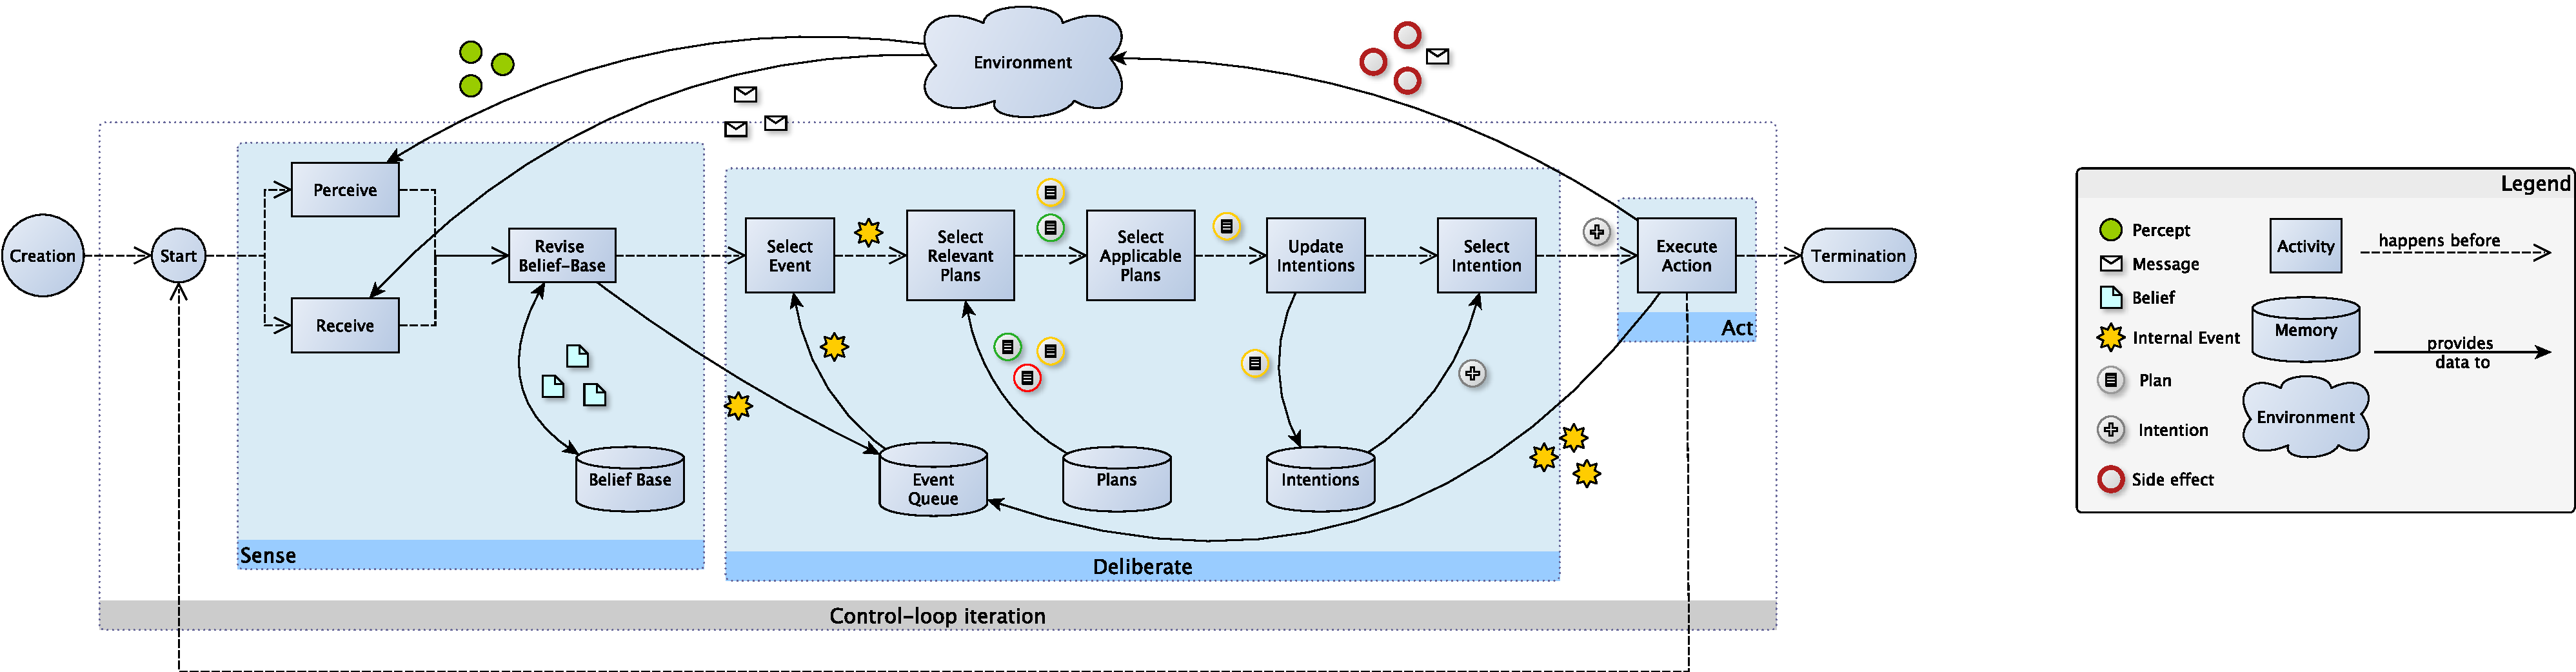
\includegraphics[width=\textwidth]{figures/jaamas26/bdi.pdf}
    \caption{
        Graphical representation of the \agentspeak{} architecture for \ac{BDI} agents.
    }
    \label{fig:bdi-architecture}
\end{figure*}

\paragraph{Control Loop}

Each \agentspeak{} agent is animated by a control-loop,
i.e., a sequence of operations
(grouped into three major phases)
that are repeated indefinitely until the agent terminates.
%
Technically speaking,
the control-loop has been implemented in so many ways
-- each one coming with a different impact on the external concurrency of the agents~\cite{BaiardiBCPOR24b} --,
but the core abstraction is always the same.

\Cref{fig:bdi-architecture} shows a graphical representation of overall architecture of an \agentspeak{} agent,
with a focus on the major phases and operations composing the agent's control loop,
and the internal/external events therein involved.
%
Roughly speaking,
the control-loop assumes that each agent has a queue of internal events manipulated as follows.
%
Each iteration of the control-loop starts with the \emph{sense} phase,
where the agent collects
\begin{inlinelist}
    \item\label{ctloop:phase:sense1} percepts
    and
    \item\label{ctloop:phase:sense2} incoming messages,
    from the environment (i.e. external events),
    \item\label{ctloop:phase:sense3} updates the beliefs accordingly
    (enqueuing events from the updated beliefs).
\end{inlinelist}
%
Next, the agent executes the \emph{deliberation} phase, where it
%
\begin{inlinelist}
    \item\label{ctloop:phase:delib1} picks one event from the queue;
    \item\label{ctloop:phase:delib2} selects a plan for handling the event,
    assigning it to some pre-existing or novel intention;
    and, consequently,
    \item\label{ctloop:phase:delib3} selects an intention to advance.
\end{inlinelist}
%
Finally, the agent executes the \emph{act} phase, where it
executes one action from the intention selected in step~\ref{ctloop:phase:delib3}.
%
The action execution may provoke further internal events,
which are then enqueued
(and therefore processed in the next iterations of the control-loop),
as well as external events,
which are delivered to the environment or other agents.

\paragraph{Execution}

The execution of a \ac{BDI} agent boils essentially down to scheduling control-loop phases
and handling events.
%
Practically,
this may vary across implementations
and be fairly different between simulations and real-world executions.
%
Specifically, defining how the control loop is scheduled
may lead to different emerging behaviours of the overall \ac{MAS} due to
which interleaving of agent's control loops is allowed by the implementation.
%
On the one side,
in simulations,
the simulator is in charge of (reproducibly) virtualizing the flow of time.
%
In this case,
`executing the \ac{BDI} system' means to advance the simulation time
while deciding which agent(s) shall execute their control-loop phases next.
%
The goal here is emulate concurrency, while keeping the execution of the agents deterministic and reproducible.
%
On the other side,
in real-world deployments,
the agents are executed by the operating system,
the flow of time corresponds to the real-world time,
and the agents are scheduled by the operating system's scheduler,
which may introduce non-determinism in the execution of the agents.
%
In this case,
the goal is to balance agents execution onto the available computational resources,
and to exploit parallelism accordingly.

% In this work,
% we focus on implementations in which the \emph{same} specification used for the real-world software
% can be used in simulation for validation purposes.
% the simulation of \ac{BDI} \ac{MAS},
% and their real-world deployment.

\subsection{Simulation Concepts: \acs{DES}, \acs{DTS}, \acs{MABS}}
\label{subsec:simulation:discrete-simulation}

We call simulation the process of replicating a real-world process
in a simplified and controlled fashion to gather insights about its behaviour.
%
Simulation can be performed by different means,
in this paper we refer to \emph{in-silico} simulation
(where the system model is described in software and executed on a computer)
of systems that feature temporal evolution.

%fidelity:
A general problem in simulation is how to ensure that the simulated system has
sufficient similarity with the real-world system it aims to replicate.
%
The degree of similarity is often referred to as the
\emph{fidelity} of the simulation~\cite{DBLP:conf/wsc/MoonH13}.
%
A related concept often used in software engineering
is the \emph{reality gap}~\cite{DBLP:conf/ecal/JacobiHH95}, which
refers to the discrepancies that may arise when transitioning
from a design to its real-world implementation.

When using simulation as a validation tool,
the reality gap can be used to refer to the differences between the behaviour of the simulated system
and of the real-world system once deployed.
%
The concepts are obviously related:
increasing the fidelity of the simulation reduces the reality gap,
and a wide reality gap is often a symptom of low fidelity.
%
In this paper we will use both concepts
-- which are valid for all kinds of simulated systems --
to discuss the trade-offs of different design choices
when simulating \ac{BDI} \acp{MAS}.

\paragraph{Main Kinds of Simulation}

% temporal model
Temporal evolution can be driven by events that happen and cause time to advance, in case of \acf{DES};
or by ``forced'' leaps forward (typically of a constant amount of time)
that cause the re-evaluation of the system state, in case of \acf{DTS}.
%
Different models of temporal evolution are suitable for different scenarios,
with \acp{DES} being generally capable of capturing more fine-grained dynamics
(for instance, stochastic chemistry~\cite{Cai2007}),
while \acp{DTS} being better at scaling and parallelisation when the phenomenon under study has a continuous nature in time
(for instance, n-body simulations~\cite{Richardson2000}).

% mabs
Simulation frameworks that rely on the notion of agent to model their domain
are called \ac{MABS}~\cite{DrogoulVM02,BandiniMV09},
of which some prominent examples in the literature include
NetLogo~\cite{Sklar07},
 Mason\cite{LukeCPSB05},
 RePast~\cite{NorthCOTMBS13},
 GAMA~\cite{Taillandier2018},
 and Alchemist~\cite{PianiniJOS2013}.
%
\ac{MABS} are designed to support the modelling of complex systems in terms of independent agents,
with the goal to replicate complex phenomena for which other models
(e.g., \acp{ODE}) are unsuitable~\cite{DBLP:books/tf/09/DrogoulMF09,Edmonds00}.

% mabs for testing bdi
As such,
\ac{MABS} are \emph{not} primarily designed to support \emph{testing of agent-based software}.
%
Indeed, they expose their own notion of agent,
typically simpler than agent abstractions devoted to programming distributed systems,
such as \ac{BDI} agents.
%
Using a \ac{MABS} framework to simulate a \ac{BDI} \ac{MAS} requires a significant effort
to either write a simplified version of the system to be tested
(at the price of losing fidelity)
or build an adaptation layer mapping the original \ac{BDI} program onto the \ac{MABS}' abstractions.


\paragraph{Simulation for \ac{BDI} \acp{MAS} Testing}
In this work,
we are interested in leveraging simulation as part of the development toolkit of \ac{BDI} \acp{MAS},
specifically to test the system's behaviour in a controlled environment ahead of time,
to discover bugs,
stress-test the system in corner cases,
measure performance,
investigate transients,
and so on.
%
To do so,
it is paramount that the \ac{BDI} specification (i.e., the program code) exercised in testing via simulation
is \emph{the same} that will be later deployed in the real-world system,
or the price paid in fidelity will hardly be acceptable
(and, as a consequence, testing via simulation will lose its potential value).
%
Although not designed for this purpose,
we argue that \ac{MABS} are the tool that most closely resembles the needs of \ac{BDI} developers.
%
As previously introduced, however,
there is a substantial abstraction gap between the two models,
filling which is part of the contribution of this work.
%
From the point of view of the time model,
\acp{DES} appear the most natural choice to simulate \ac{BDI} agents,
as they are event-driven in nature as discussed in \Cref{ssec:computational-bdi}.
%
One of the contributions
of this work is showing how the control-flow events of \ac{BDI} agents can be mapped
onto \ac{DES} engine events,
and what are the implications of alternative design choices.

In exploring the trade-offs, we also consider practical considerations
that affect how simulation supports software validation in early development stages.
%
In many scenarios,
simulation could be used to explore a cheap virtual prototype of the system,
even before a real counterpart exists~\cite{DBLP:journals/jos/FortinoN13,DBLP:journals/csse/FortinoGR05}.
As development progresses, the expected fidelity of the simulation should naturally increase, improving its usefulness as a validation tool.
%
Achieving higher fidelity, however, often requires more fine-grained models,
which come with greater computational cost.
This leads to an inevitable trade-off between accuracy, development time, and simulation duration.
%
Different phases of the engineering process may therefore call for different fidelity levels: fast, low-detail simulations to rapidly test ideas early on, and slower, high-detail simulations later when behaviour must be assessed more thoroughly.

\section{\ac{BDI} Agents Simulation Methods}
\label{sec:simulation:related-works}

To achieve \ref{rq:methods},
in this section,
we investigate the state of the art of \ac{BDI} agents simulation.

The idea of testing \acp{MAS} dynamics via simulation
dates back to the early 2000s~\cite{uhrmacher_simulation_2002}.
%
However,
despite recognizing the relevance and complexity inherent in testing \acp{MAS}~\cite{miles_why_2010,nguyen_testing_2011},
and the existence of methodologies that include simulation for \ac{MAS} development~\cite{cossentino_passim_2008},
there are not many tools that effectively allow one
\emph{
    ``to execute agents as they are and to switch arbitrarily between execution in the real environment and the virtual test environment''
}\cite{uhrmacher_simulation_2002}.
%
The lack of dedicated simulation tools
is especially relevant for \ac{BDI} agents,
whose agents' lifecycle is richer compared to other models.

This seamless switching is the primary goal for our work~\cite{DBLP:conf/dsrt/Baiardi24}.
%
In fact,
keeping the \emph{same} agent specification
ensures that simulation results are not artefacts induced
by the software translation into a simulation-compatible model.
%
Additionally,
if the specification is the same,
issues discovered at deployment time that were not evident during testing
will be at most imputable to the abstraction gap of the environment model.
%
A recent work has tackled this problem for non-\ac{BDI} agents~\cite{Briola2025},
by developing a simulation environment for the JADE \ac{MAS} platform~\cite{DBLP:books/wi/BellifemineCG07}.
%
The work focuses on achieving portability of the same agent behaviour between simulation and real-world execution,
by implementing a simulation environment that mimics the JADE run-time environment.
%
We exclude this work from our comparison, as JADE agents are not \ac{BDI}-based.

% and generally not captured by (much simpler) models featured in \ac{MABS};
% thus
% making the idea of simulating \ac{BDI} agents in a \ac{MABS} framework
% burdening and impractical,
% as the agent interpreter needs to be reimplemented from close to scratch.
%
% The options at hand for \ac{BDI} developers are limited to~\cite{singh_integrating_2016}:
Several attempts to use simulation as a testing tool for \ac{BDI} \acp{MAS} have been done in the past,
falling into the three main categories~\cite{singh_integrating_2016},
described below.

\newcommand{\relatedExtendFramework}{(1)}
\newcommand{\relatedExtendSimulator}{(2)}
\newcommand{\relatedMiddleware}{(3)}

\paragraph{\relatedExtendFramework{} Adding Simulation Features in \ac{BDI} Frameworks}

Agent frameworks can, in principle,
be modified so that the \ac{MAS} environment is replaced by a simulated one.
%
In practice, this operation may be difficult
because it depends on the \textit{concurrency model}~\cite{BaiardiBCPOR24} adopted by the framework
and how customizable the framework is.
%
Nevertheless,
some \ac{BDI} programming frameworks
include simulated execution.
%
For instance,
\jason{}~\cite{HubnerB09} allows a \ac{DTS} execution mode
with steps that execute one reasoning cycle for each agent,
and in~\cite{ricci_exploiting_2020} is present a proposal to apply \ac{DES} to \jacamo{}.

\paragraph{\relatedExtendSimulator{} Implementing \ac{BDI} Features in Simulators}

As discussed in \Cref{subsec:simulation:discrete-simulation},
the agent model in \ac{MABS} simulators are simpler than \ac{BDI} agents,
thus,
their execution requires a reimplementation of the agent interpreter on top of the simulation engine.
%
\ac{BDI} extensions exist for several popular \ac{MABS}.
%
Some basic \ac{BDI} and FIPA~\cite{o1998fipa} communication libraries
have been implemented in NetLogo~\cite{Sklar07}
for educational purposes~\cite{sakellariou_enhancing_2008},
and
a \ac{BDI} layer has been implemented on top of the GAMA~\cite{DrogoulACGGMTVVZ13} platform
to support social simulations with cognitive models~\cite{TaillandierBCAG16}.
%
Other approaches rely on the \ac{DEVS} formalism to represent \ac{BDI} reasoning,
such as JAMES~\cite{uhrmacher1998agents}.

\paragraph{\relatedMiddleware{} Integration through Synchronisation}

Finally,
an approach is the integration of an existing \ac{BDI} framework with an off-the-shelf simulator.
%
This is typically achieved through some form of synchronisation,
either through inter-process communication
or shared memory.
%
A generic framework for such integration is proposed in~\cite{singh_integrating_2016}
suggesting the adoption of a standard interface to map \ac{BDI} agents with \ac{MABS} agents;
and showing validation through different combinations of \ac{BDI} and \ac{MABS} platforms.
%
In~\cite{davoust_architecture_2020},
instead,
a shared memory approach is used to make \jason{} agents interact with the simulated environment asynchronously,
reducing the time the simulation engine spends \emph{waiting} for the agent reasoning.

\paragraph{Remarks}

Categories \relatedExtendFramework{} and \relatedMiddleware{} would preserve the same code for the agent behaviour.
%
Category \relatedExtendFramework{},
besides requiring a considerable effort to build a simulation engine from scratch,
would hardly match existing state-of-the-art simulators
in terms of performance,
environment modelling,
visualization,
and data export tools.
%
Using strategy \relatedMiddleware{}, as we discuss in more detail in \Cref{sec:simulation:bdi-over-des},
can have important consequences on the reality gap with respect to the real-world execution.
%
Depending on how synchronisation is achieved,
assumptions on agent executions may be introduced implicitly,
possibly leading to unreliable results.
%
Simulating the behaviour of an existing \ac{MAS} following strategy \relatedExtendSimulator{}
requires to rewrite the agents' behaviour using the simulator's \ac{API}.
%
This is critical,
as it is hard to guarantee that the software will be the same,
and costly to realize and maintain.

In this paper,
we take an approach that sits in between these categories.
%
We do start from an existing \ac{BDI} framework and an existing simulator,
but instead of relying on some form of synchronisation,
we make the simulator run \ac{BDI} agents directly.
%
This is similar to the approach used to
support social simulations by integrating MASON~\cite{LukeCPSB05} with \jason{}~\cite{BordiniHW2007}
by incorporating the \jason{}'s interpreter within MASON
to directly execute agents written in \agentspeak{}~\cite{caballero2011eaai}.
%
%This achieved the goal of allowing simulation developers
%to write agent behaviour uisng regular \jason{} syntax,
%with the side-effect of enabling to test \jason{} programs in a simulated setting
%without the need to change the codebase.
%
The main difference of our proposal is in the scope:
we do not mean -- as \cite{caballero2011eaai} -- to build better social simulations using \ac{BDI} agent modeling,
rather,
 we want to provide a toolkit to test the behaviour of deployable \ac{BDI} software systems.
%
This difference in scope makes the execution of a complete reasoning cycle at each simulation step as done in~\cite{caballero2011eaai}
not viable under the fidelity point of view,
as we will discuss in \Cref{sec:simulation:bdi-over-des} and demonstrate in \Cref{sec:simulation:evaluation}.

\section{Integrating \ac{BDI} and \ac{DES}}
\label{sec:simulation:bdi-over-des}

% In this section,
% we focus on the problem of running a \ac{BDI} \ac{MAS} specification over a \ac{DES} platform
% with no change to the original specification,
% much like the execution of a centralised software in debug mode does not impact
% the application code.
% %
% In principle,
% the underlying platform should simply be swapped
% and provide different implementations of the same \ac{API}
% the \ac{BDI} software expects.
% %
% However,
% for this swap to be realisable,
% there are several critical aspects that need special care:
% %
% \begin{inlinelist}
%     \item the \emph{granularity} of the \ac{BDI} lifecycle events as supported by the simulation/execution platform;
%     \item the \emph{interaction} with non-\ac{BDI} sources of change;
%     \item the \emph{determinism} of the execution platform,
%     which impacts reproducibility in simulated scenarios;
%     \item the spatial nature of the environment,
%     and, finally,
%     \item inter-agent communication,
%     for which simulated backends can use shared memory instead of (de)serialisation.
% \end{inlinelist}

In this section
(and, more specifically, in \Cref{sec:simulation:portable-agent-specifications}),
we discuss how to allow
for testing the behaviour of \ac{BDI} agents systems
in a simulation environment,
without changes to the codebase of the \ac{MAS} specification (\ref{rq:abstract-spec}).
% we now discuss the implication of achieving that objective.
%
In particular,
as mentioned in \Cref{subsec:simulation:discrete-simulation},
we are interested in studying the exploitation of \ac{DES} to serve this purpose (\ref{rq:des}).
%
At the intuition level,
this should be possible,
as the events generated by the \ac{BDI} agent's control loop
can be scheduled in a \ac{DES} engine and interleave with all other simulation events.

In principle,
given a \ac{MAS} made up of
\begin{inlinelist}
    \item agents' behavioural specifications,
    \item an environment abstraction to handle perceptions, actions, and communication,
    and
    \item an execution platform to run the system,
\end{inlinelist}
one could retain the agents specification and swap the remainder with a simulator
to achieve the desired objective.
%
However, this task is \emph{deceptively simple}:
in the following subsection we will analyse how each of these elements
needs to be carefully designed to make such swap possible.

Before proceeding,
let us clarify that,
in the remainder of this paper,
we specifically focus on agents whose behaviour is \emph{manually} specified beforehand by human developers
-- such as \ac{BDI} agents --
rather than \emph{learned} autonomously%
---e.g., via reinforcement learning.
%
In principle, though, similar considerations apply for learning agents,
provided that learning occurs \emph{online}\footnotemark
-- meaning \emph{during} the agent's interaction with the environment --
as opposed to \emph{offline} training%
---which occurs \emph{before} agents' execution.

\footnotetext{
    If an agent's behavioural specification includes some form of \emph{online} learning capabilities,
    (e.g., by implementing Q-learning~\cite{Watkins1992}),
    then
    the agent would be able to learn from its experience in the simulated environment
    as it would do in the real-world deployment.
    %
    However,
    we acknowledge that modern approaches to reinforcement-learning
    (e.g., deep reinforcement learning~\cite{FigueiredoPrudencio2024})
    commonly rely on an \emph{offline} training phase,
    which leverages the simulation environment to generate training data and update the agent behaviour
    (i.e., the learned \emph{policy})
    accordingly.
    %
    This training phase is outside the scope of this work,
    but given the final specification of the agent behaviour
    (e.g., a trained neural network implementing a policy),
    our assumptions discussed at the beginning of \Cref{sec:simulation:bdi-over-des} still apply.
    %
    In fact,
    the learned policy would simply work in the target environment
    (no matter whether it is simulated or real-world),
    provided that the agents' perceptions and actions are properly abstracted
    % to feed as inputs of the neural network and to enact its outputs.
    and wired to the neural network's input and output layers.
}

\subsection{Portable Agent Specifications}
\label{sec:simulation:portable-agent-specifications}
% We have already established in \Cref{subsec:BDI-agents}
% that the control flow of a \ac{BDI} agent can be considered event-driven.

We have established that the main goal of this work is to allow
the same \ac{BDI} agent specification to be executed
both in simulation and in real-world deployments.
%
The technical implication of this goal is to ensure that the agent code
is \emph{portable} i.e., it depends solely on platform-agnostic \acp{API},
which can be implemented differently depending on the execution context
(simulation or real-world).

Platform-specific implementations
-- at least, one for real-world deployments and another for simulation --
must be provided for such a platform-agnostic \ac{API}.
%
We refer to these implementations
as the \emph{interpreters} of the \ac{BDI} agent specification,
which are responsible for executing the agent code
by relying on the underlying platform functionalities.
%
The two interpreters may of course differ in their implementations,
yet both should guarantee the \agentspeak{} semantics is preserved.
%
In this regard,
a good practice is to let the two interpreters share as much code as possible:
ideally implementing the agent's control loop in a shared library,
which allows for plugging in different platform-specific functionalities.

Given the role of environment abstractions
for \ac{MAS} programming~\cite{weyns2007aamas}
that can be used to abstract agents from the execution context%
-- ranging from distributed systems~\cite{IssicabaRPB17} to robotics~\cite{pantoja2016atal,moro2022paams} --%
we discuss what are the fundamental requirements
to design an environment \ac{API}
that allows for portable \ac{BDI} agent specifications
that can seamlessly run on a simulation platform.
%
Namely, the environment \ac{API} must be designed to abstract the following functionalities.


\paragraph{Time}
Agent behaviour may depend on the passage of time.
%
Hence, agents may need to observe the current time,
usually through the system's clock in a real-world deployment.
%
In simulation, however, the flow of time is virtualized and controlled by the simulator,
and it usually does not correspond to real-world time.
%
Thus, access to \emph{time-dependent} functionalities
(e.g., timestamps, timeouts, delays)
must not be implemented by accessing system-level time primitives directly.
%
Accessing the system's clock, or using sleep functions
must be avoided in the agent code,
and instead the environment \ac{API} must provide the necessary functionalities
to access the current time
or to schedule timeouts and delays.
%
It will then be the responsibility of the integration with the simulation platform
to provide a proper implementation of such functionalities
upon the simulator's notion of time,
guaranteeing semantic correspondence with the real-world counterpart.


\paragraph{Randomness}
Sometimes,
the agents' behaviour may require a degree of \emph{non-determinism}%
---e.g., using random number generators.
%
In simulation,
to ensure reproducibility of simulation,
all non-determinism must be controlled by the simulator.
%
Thus,
similar to time-related primitives,
random number generation
must be provided by the environment \ac{API}.
%
Reproducibility is especially significant when simulations are a mean
to debug anomalies.
When debugging, any two executions with the same random seed
\emph{must} produce the same sequence of events,
otherwise, the original issue may not re-occur,
or, worse, may manifest differently,
making understanding and fixing the problem much harder---%
an issue known in the software engineering community as \emph{flaky behaviour}\cite{DBLP:journals/tosem/ParryKHM22}.


\paragraph{Perceptions and Actions}
Agents' interaction with the environment
happens through perceptions and actions.
%
On the one side, the environment \ac{API} must provide functionalities
to perceive the state of the environment entities and deliver perception \emph{events}
to the agents.
%
On the other side, the environment \ac{API} must encapsulate all the actions
that agents can take to influence the environment state.
%
This level of separation is the most common in \ac{MAS} programming frameworks,
but it is worth stressing its importance
when the goal is to run the same agent specification
both in simulation and in real-world deployments.
%
In (\Cref{ssec:simulation:design-simulated-environment})
we will discuss in depth the implications of this abstraction when
discussing how to bind the \ac{BDI} environment \ac{API}
to a \ac{DES} simulation platform.



\paragraph{Communication}
Agents in a \ac{MAS} often need to communicate with each other.
%
To support inter-agent
communication, the environment \ac{API} must provide functionalities to send and receive messages.
%
Real-world (distributed) deployments rely on network protocols
(e.g., HTTP, MQTT, XMPP, etc.),
and although in principle they can be used in simulation as well,
a typical choice driven by performance and improved experimental control
is to abstract them away and provide direct control over relevant control variables
(latency, message/package loss, retransmissions).
%
Typically,
in \ac{MAS}
the environment acts as a \emph{relay} for messages,
and messages might be subject to some sort of \emph{propagation} mechanism.
%
The way messages are propagated may depend on the scenario,
for instance,
taking into account the environment topology by
limiting the delivery of messages to \emph{reachable} destinations,
or
introducing some form of \emph{delay}
or \emph{loss}
in the delivery of messages
to better match with the expected real-world environment dynamics and
stress the properties of the system under different conditions.
%
Again, failing to abstract communication functionalities
would make impossible to simulate the system,
as the simulator would need to rely on the underlying network stack to deliver messages between agents,
which would make the simulation results unreliable and non-reproducible.


\subsection{Design of the Simulated Environment}
\label{ssec:simulation:design-simulated-environment}

Having defined the requirements for portable \ac{BDI} agent specifications (\Cref{sec:simulation:portable-agent-specifications})
by encapsulating all platform-specific functionalities
into a generic environment \ac{API},
we now focus on the implications of implementing such \ac{API}
on top of a \ac{DES} simulation platform.
%
These considerations are generally valid for any simulation environment
that aims to support the typical application scenarios of (\ac{BDI}) \acp{MAS},
i.e., distributed systems where agents interact with each other
and with a dynamic environment, possibly featuring
entities that can move in a physical space.
%
Although not specific to \ac{BDI} agents,
we still discuss these aspects,
as they set requirements and constraints in the choice of the simulation platform
and in the design of the simulation environment
that will host the \ac{BDI} \ac{MAS} under test.

The most important difference between real-world deployments and simulations
concerns the way \emph{external} events are delivered to the agents.
%
In this section we focus on the modeling of such events,
leaving the discussion on
the scheduling of \emph{internal} events to \Cref{ssec:simulation:granularity}.

The \ac{BDI} model already assumes agents to be reactive to the external events they perceive.
%
In real-world deployments,
developers can wire \ac{BDI} agents' perceptions and actions to physical sensors and actuators
or connect the agents with I/O peripherals and external services.
%
External events just occur, and agents either perceive or cause them.
%
Instead,
in simulation,
external events are delivered to the agents by the simulator,
and therefore require additional modelling and programming efforts.

% The design of a simulated environment to test a \ac{MAS} is then threefold.
% %
% It must
% \begin{inlinelist}
%     \item deliver the same events the agent may receive in the real-world execution,
%     \item provide the same \ac{API} expected by the agent codebase to act on the environment and exchange messages,
%     and
%     \item be able to replicate the dynamics of the real-world environment.
%     %with the highest possible fidelity.
% \end{inlinelist}


\paragraph{Topology and Situatedness}

\ac{BDI} \acp{MAS} can be deployed either in physical or virtual environments.
Depending on the nature of the target scenario,
to accurately replicate the real-world mechanisms,
the simulation environment must support the notion of \emph{situatedness} (cf. Wooldridge \cite{Wooldridge00}),
that is crucial for all kinds of agents
and determines the range of observability and influence of the agents.
%
In some cases,
for instance when the target scenario features robots or mobile devices,
agents need to be further \emph{embodied}~\cite{brooks1991ijcai},
making them directly part of the environment,
and observable to other agents.

While in real-world deployments the space and topology of a \ac{MAS} is a \emph{constraint},
in simulation they are aspects to be modelled and programmed;
and the programming efforts might vary significantly depending on the target application.
%
When agents are expected to be deployed on mobile devices,
the simulation can use manifolds
(e.g., 3D spaces or city maps)
where location and distance can be defined.
%
In other cases,
for instance in \emph{networked} systems,
manifolds are not relevant,
but the \emph{network topology} is.
%
These are \emph{logical} environments,
in which entities are located into nodes of a graph,
and distances are computed as functions of the paths connecting them.
%
In some applications,
these aspects mix:
for instance,
a wireless sensor network may feature geographically \emph{situated} devices
for which a logical topology can model the communication channels
(e.g., based on the relative distance of the devices).
%
In any case,
a notion of \emph{closeness} is necessary
to limit the perception range and influence of agents,
whose specific reification
should be left to the simulation implementation,
as it
is scenario-dependent.

These aspects are important to consider when implementing the environment \ac{API}
on top of a \ac{DES} platform.
For instance, the perception range influences which events
should deliver perceptions to the agents,
and the topology may affect how messages are propagated in the environment.
%
These parameters should be carefully modelled in the simulation
and can be used as variables to explore different simulated scenarios.


\paragraph{Environment Dynamics}

In any non-trivial scenario,
there will be events generated externally to the \ac{BDI} agents,
as real-world environments are typically dynamic
(i.e., they change over time)
or feature some form of stochastic behaviour
(e.g., package loss in networked systems).
%
Movement,
communication,
and, more generally,
any phenomena that span over time affecting the agents' perceptions,
must be modelled into events with appropriate time distributions.
%
These events must be modelled in simulation
and properly interleave with the agents' reasoning cycle.
%
The interleaving between agents' internals and other events
essentially determines how agents are executed in the simulation,
as we discuss in the next section.
%
The design of the environment dynamics
allows one to implement the \ac{API} used by the agents to
perform actions that have effects on the environment state,
but also to model external sources of change
completely independent of the agent behaviour,
that may challenge the \ac{MAS} execution,
thus stressing its properties
in different scenarios.
%
As for any simulation, the more accurate the model of the environment dynamics,
the higher the fidelity of the simulation will be.

\subsection{Mapping the \ac{BDI} Execution on a Simulator}
\label{ssec:simulation:granularity}

% Import image granularity.pdf
\begin{figure*}
    \centering
    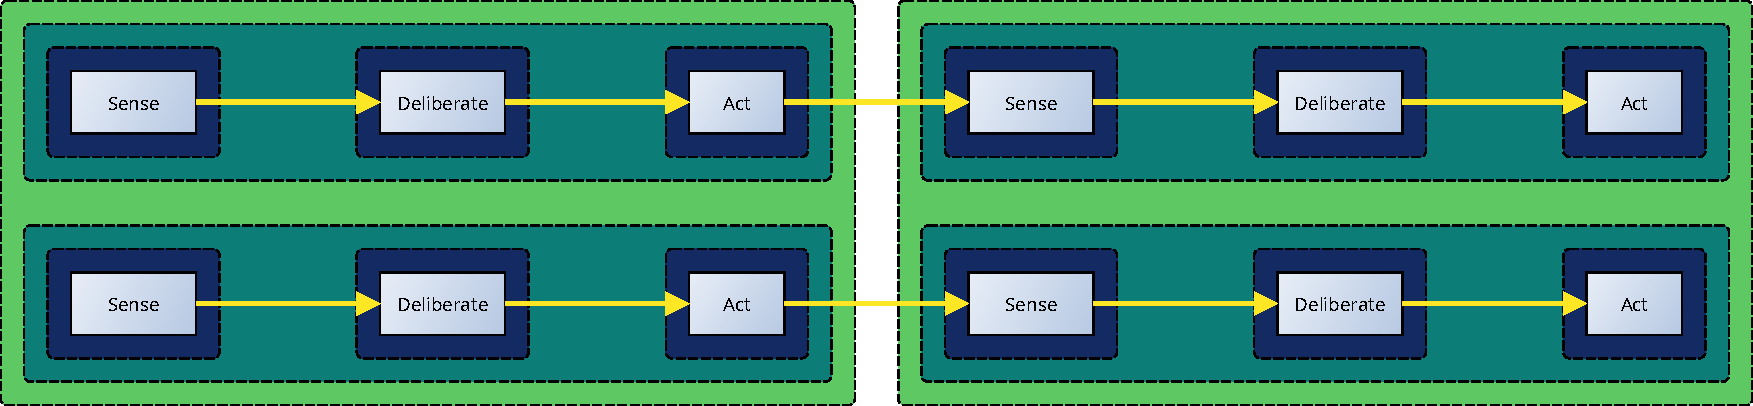
\includegraphics[width=0.8\textwidth]{figures/jaamas26/granularity.pdf}
    \caption{
        Granularities for atomic \ac{BDI} events.
        Yellow arrows are causal links.
        In \acs{AMA} (light green) an event is a run of all control loops of the whole \ac{MAS};
        it implicitly synchronises all agents.
        In \acs{ACLI} (emerald) an event is a single control loop iteration of a single agent,
        preventing phase interleaving.
        In \acs{ACLP} (dark purple), single control loop phases of every agent can interleave.
        \acs{ABE} is not shown as it is indistinguishable from \acs{ACLP} at the agent level.
    }
    \label{fig:granularity}
\end{figure*}

Mapping \ac{BDI} events in a \ac{DES}
to achieve \ref{rq:des}
requires an understanding
of which events are \emph{atomic} in a \ac{BDI} system execution.
%
Then,
any collection of these atomic events can be mapped to a single \ac{DES} event,
defining the mapping \emph{granularity},
and thus defining which \ac{BDI} groups of events can interleave with other simulation events.
%
The granularity influences the \emph{fidelity} of the simulation,
and is similar to choosing the external concurrency model~\cite{BaiardiBCPOR24} of a \ac{BDI} system upon deployment.
%
The granularity does not affect the individual agent program semantics
(the specification of behaviour is the same),
but may influence the collective dynamics of the \ac{MAS}
due to the interleaving of individual agent actions.
%
Coarse-grained mappings (i.e. multiple agents events mapped to one simulation event) introduce implicit synchronisation that suppresses possible interleavings, thus potentially hiding timing-dependent faults, race conditions, message races, and sensor (or actuators) delays that would happen in a real deployment.
%
Finer-grained (i.e. one agent event mapped to one simulation event)
mappings expose asynchrony and delays,
increasing fidelity and reducing the reality gap,
but at the cost of a more difficult integration mapping.
%
\Cref{fig:granularity} summarises the options that we discuss below,
showing the trade-offs for each choice.

\subsubsection{\acf{AMA}}\label{subsubsec:simulation:ama}

Each \ac{DES} event corresponds to a \emph{full} control-loop iteration of \emph{all} agents in the system,
making it the most coarse-grained option.
%
This approach is adopted in~\cite{HubnerB09} and~\cite{caballero2011eaai},
which use \ac{DTS},
and it is similar to the one proposed in~\cite{singh_integrating_2016},
which advances the simulation only after all agents
are \emph{idle}.
%
One obvious consequence of this choice is that
all agents in the \ac{MAS} run at the same \emph{frequency},
thus inducing implicit synchronisation,
and discarding all the effects caused by possible
\emph{interleaving} agents' actions.

\subsubsection{\acf{ACLI}}\label{subsubsec:simulation:acli}

Each \ac{DES} event corresponds to a \emph{full} control-loop iteration of a \emph{single} agent,
making this option slightly more fine-grained than \ac{AMA}.
%
In this case,
arbitrary interleaves among agents' \emph{actions} are possible,
but not among different agents' control-loop \emph{phases}.
%
This option does not allow modelling different durations for different phases of the control loop,
for instance,
it cannot be captured a situation in which
deliberation takes too long and makes the sensing phase outdated before an action is taken.

\subsubsection{\acf{ACLP}}\label{subsubsec:simulation:aclp}

Every single \emph{atomic phase}
(sense, deliberate and act)
is represented as a \ac{DES} event.
%
This option preserves the behaviour of concurrent or distributed \ac{BDI} agents,
allowing phases to interleave across different agents,
thus capturing complex inter-agent concurrency patterns.

\subsubsection{\ac{ABE}}\label{subsubsec:simulation:abe}

Each \ac{BDI} event is mapped to a single \ac{DES} event.
%
This is the finest-grained option,
first proposed in~\cite{ricci_exploiting_2020}.
%
The approach has value for investigating the internals of the agent execution platform implementation,
e.g., to verify the correctness of the \ac{BDI} interpreter implementation
and its degree of parallelism,
but,
from the point of view of an observer of the \ac{MAS},
this model and \ac{ACLP} are indistinguishable,
as the phases of the control loop of each agent are atomic.
%
For this reason, in the remainder of the paper,
we will consider \ac{ABE} to be subsumed by \ac{ACLP}.

\subsection{Tool Requirements for the Integration}
\label{ssec:simulation:requirements}
Following the key features outlined in the sections above,
the tools to be adopted for the integration must provide:
\begin{itemize}
    \item neat \emph{modularisation} of the \ac{BDI} execution engine,
    to simplify its replacement with the simulation engine;
    \item abstract \emph{``external concurrency''} model~\cite{BaiardiBCPOR24},
    to allow for different granularities of the \ac{BDI} events
    -- and therefore different fidelity levels --
    in simulations;
    \item \emph{extensibility} of the \ac{DES} framework,
    which must accommodate the \ac{BDI} framework's abstractions with no major changes;
    \item \emph{simulation model} featuring locality, position, and communication channels,
    to support simulating agents situated in physical or logical spaces;
    \item native \emph{integration} (i.e., same runtime) between the \ac{BDI} framework and the simulator,
    to avoid the additional burden of inter-process communication mechanisms.
    % and
\end{itemize}

\section{Prototype: \jakta{} over \alchemist{}}
\label{sec:simulation:prototype}

% \samu{qua discuterei meglio il "senso" di questo prototipo, sottolineando che è un prototipo della feasibility e una dimostrazione che applicando le accortezze discusse sopra si riesce ad ottenere il risultato. Il mapping proposto è specifico per le tecnologie, ma la metodologia e le considerazioni sopra sono generali e si possono applicare a framework diversi a patto che si identifichi il modo di individuare e schedulare l'esecuzione degli agenti}

To demonstrate the feasibility of the ideas discussed in the previous sections,
and in order to achieve \ref{rq:sim-integration},
here we present a proof of concept implementation of a \ac{BDI} interpreter supporting both real-world and simulation execution.

In particular,
our discussion revolves around the \jakta{} \ac{BDI} framework~\cite{BaiardiBCP23},
which \emph{already} supports real-world execution of \ac{MAS} as concurrent applications,
and it allows for plugging in different \emph{concurrency models}~\cite{BaiardiBCPOR24b}.
%
Put simply,
\jakta{} is a \ac{BDI} interpreter which lets developers customise the way agents' control loop iterations -- as well as agents' perceptions and actions -- are executed.
%
For the sake of conciseness,
in this section,
we only show how \jakta{} can be extended to support one more way to run agents,
namely:
in a simulated world,
as created by the \alchemist{} simulator~\cite{PianiniJOS2013}.
%
The interested reader can refer to~\cite{SNCS:JaktaJournal} for a more detailed discussion on \jakta{},
and its support to \ac{BDI} agents in real-world deployments.

Further motivations exist for the technological choice of \jakta{} and \alchemist{},
as we discuss in \Cref{ssec:simulation:requirements} and in \Cref{ssec:simulation:choices}.
%
As the reader will notice,
our prototype is tailored on these two technologies,
and the discussion in this section is specific to them.
%
However,
we believe that our experience has a general value:
not only it proves that \ac{BDI} systems' execution can be swapped between real-world deployments and \ac{DES} simulation
without changing the \ac{MAS} specification,
but it also allows us to study the impact of the many simulation granularity levels (see \Cref{ssec:simulation:granularity})
on the validation of a \ac{BDI} system.
%
This is indeed the purpose of \Cref{sec:simulation:evaluation}.

Technically speaking,
our prototype is implemented
as a stand-alone module in the \jakta's codebase,
named \texttt{alchemist-\allowbreak{}jakta-\allowbreak{}incarnation},
which imports simulator's \ac{API}
and allows developers to plug their \ac{BDI} specification
to be executed in a simulated environment.
%
The source code is publicly available\footnote{
    \url{https://github.com/jakta-bdi/jakta}
    % \url{https://anonymous.4open.science/r/jakta-sim-4C2F}
}
under a permissive licence
and archived on Zenodo~\cite{zenodojaktajaamas}
for future reference.

%\subsection{Selection of the \ac{BDI} and {DES} technologies}

\subsection{Design and Technological Choices}
\label{ssec:simulation:choices}
In line with the requirements in \Cref{ssec:simulation:requirements},
we selected the \alchemist{} simulator
and the \jakta{} \ac{BDI} framework
also because they both run on the \ac{JVM} and are therefore interoperable.
%
\alchemist{} is designed with extensible base abstractions,
thus allowing for reasonably straightforward integration with other stand-alone tools;
indeed,
it has been used in the past to simulate programmable tuple spaces~\cite{zambonelli2015percom},
biochemical systems~\cite{MontagnaSAC2012},
and aggregate programming languages~\cite{PianiniSAC2015,DBLP:journals/softx/CasadeiVAP22}.
%
Complementarily,
\jakta{} has been designed to be easily adaptable to different execution engines.
%
So,
bridging the two technologies is a matter of implementing a new \emph{incarnation} in \alchemist{}
that can run \jakta{} agents.
%

\paragraph{\alchemist{}}

\alchemist{}~\cite{PianiniJOS2013} is a general-purpose \ac{DES}
originally conceived to simulate bio-inspired systems,
from which it inherits the metaphors and terminology in use to this day.
%
In the remainder of this discussion,
terms in \texttt{typewriter font} represent names of existing software entities,
whose name has been used verbatim, as found in the \ac{API}.

In \alchemist,
the simulated model entry point is the \texttt{Environment},
which represents a Riemannian manifold\footnote{A Riemannian manifold is
a generalised Euclidean space that can be curved
(useful to support geospatial data),
discontinuous
(useful to model inaccessible areas),
and for which the distance between two points $\overline{AB}$ may depend on the direction: $\overline{AB}\neq\overline{BA}$
(useful to implement asymmetric navigation, e.g., on street maps with one-way roads).}.
%
The \texttt{Environment} is populated by \texttt{Node}s, which
\begin{inlinelist}
    \item can be equipped with arbitrary \texttt{NodeProperty}s
    \item have a \texttt{Position} in space,
    \item can be programmed with \texttt{Reaction}s,
    \item can be connected to other \texttt{Node}s via a \texttt{LinkingRule} to form \texttt{Neighborhood}s,
    \item can contain \texttt{Molecule}s (data identificators),
    each with an associated \texttt{Concentration} (data value).
\end{inlinelist}

Events in \alchemist{} are called \texttt{Reaction}s,
as they were originally conceived to simulate chemical reactions.
%
\texttt{Reaction}s in \alchemist{} extend the concept of reaction from chemistry.
%
Instead of being defined by a set of reactants that
transform into products at a rate defined by the \emph{law of mass action},
\texttt{Reaction}s in \alchemist{} are more generally defined as
collections of conditions, that, when satisfied,
trigger a set of actions according to an arbitrary \emph{rate equation}
which depends on the observable state of the \texttt{Environment}
and a provided \texttt{TimeDistribution}.

The concept of \texttt{Concentration} in \alchemist{} can be reified
in arbitrary data types.
Different types of \texttt{Concentration} may lead to a different semantics
for \texttt{Molecule}s, \texttt{Condition}s, \texttt{Action}s, \texttt{Reaction}s,
and any other abstraction depending on them,
thus allowing for different \emph{data models},
and providing a flexible and straightforward way to
bridge \alchemist{} with other tools.
%
Every set of abstractions defining a coherent semantics
for these entities is called an \texttt{Incarnation}
in the simulator jargon.
%
At the time of writing,
\alchemist{} provides several incarnations
for different application domains,
including
bio-chemical systems~\cite{MontagnaSAC2012},
networked tuple spaces\cite{zambonelli2015percom},
and aggregate programming via Protelis~\cite{PianiniSAC2015} and Scafi~\cite{DBLP:journals/softx/CasadeiVAP22}.

An \alchemist{} simulation is configured using a YAML file,
which specifies the \texttt{Environment} type,
the \texttt{Node}s to populate it with,
their initial \texttt{Molecule} concentrations,
the \texttt{LinkingRule} that connects them,
and any \texttt{Reaction}s to be executed.
%
When the simulation starts,
\alchemist{} loads the configuration file and instantiates
the specified \texttt{Environment} and its contents.

\paragraph{\jakta{}}
\label{par:jakta}

\jakta{}~\cite{SNCS:JaktaJournal} is a Kotlin-based modular \ac{BDI} framework.
%
Each agent in a \jakta{} \ac{MAS} is equipped with an \texttt{AgentLifecycle} which implements the \ac{BDI} control loop.
%
\jakta{} cleanly separates the definition of the agents' behaviour from the execution platform
in charge of executing the agents' control loop phases,
thus allowing different concurrency models for agents to be plugged in.
%
\jakta's environments (not to be confused with \alchemist{}'s \texttt{Environment}s)
are lightweight abstractions that handle
perceptions, communications, and interaction with the external world.
%
\acp{MAS} in \jakta{} are programmed through a Kotlin \ac{DSL},
which provides an expressive, type-safe, and
\ac{IDE}-friendly way to define agents' beliefs, goals, and plans.
%
Indeed, by leveraging Kotlin as the host language,
\jakta{} programs are regular Kotlin applications,
which may lower the entry barrier for developers familiar with mainstream programming languages
(Kotlin is the reference language for Android development\footnote{
    ``Android’s Kotlin-first approach'', archived 2024-02-15 \url{https://archive.is/EtWqn}
})
and are thus natively supported by any \ac{IDE} supporting Kotlin,
significantly lowering the maintenance cost.

\paragraph{Multiple granularity support}
% \samu{RIVEDERE QUESTA SECTION ORA NON FILA COL RESTO}
% GC: il titolo era fuorviante, l'ho cambiato

As discussed in \Cref{ssec:simulation:granularity},
the mapping between the \ac{BDI} framework and the \ac{DES} simulator
can be realised with different granularity.
%
We implemented multiple granularities in our prototype
to show how each of them
impacts on the tested behaviour of a \ac{BDI} software.
%
We implemented all those introduced in \Cref{ssec:simulation:granularity} but \ac{ABE} because,
as previously discussed,
its behaviour is indistinguishable from \ac{ACLP}
and supporting it
while retaining real-world deployment capability for \jakta{} specifications
would have been highly impractical\footnotemark.
%
\footnotetext{
        To support \ac{ABE},
        the \jakta{} interpreter should be modified
        to expose each atomic event as a schedulable unit of execution.
        %
        While this is feasible in principle,
        the effort required is not justified by the benefits,
        as \ac{ABE} does not provide any additional value
        with respect to \ac{ACLP}.
}

\paragraph*{}

Driven by these choices,
in the next subsection,
we proceed to identify the modelling abstractions of the two technologies
and we describe how they have been mapped
in order to merge the \jakta{} framework into the \alchemist{} simulator.

\subsection{\ac{BDI} \acp{MAS} in \alchemist{}}\label{subsec:simulation:mapping}

\begin{figure}
    \centering
    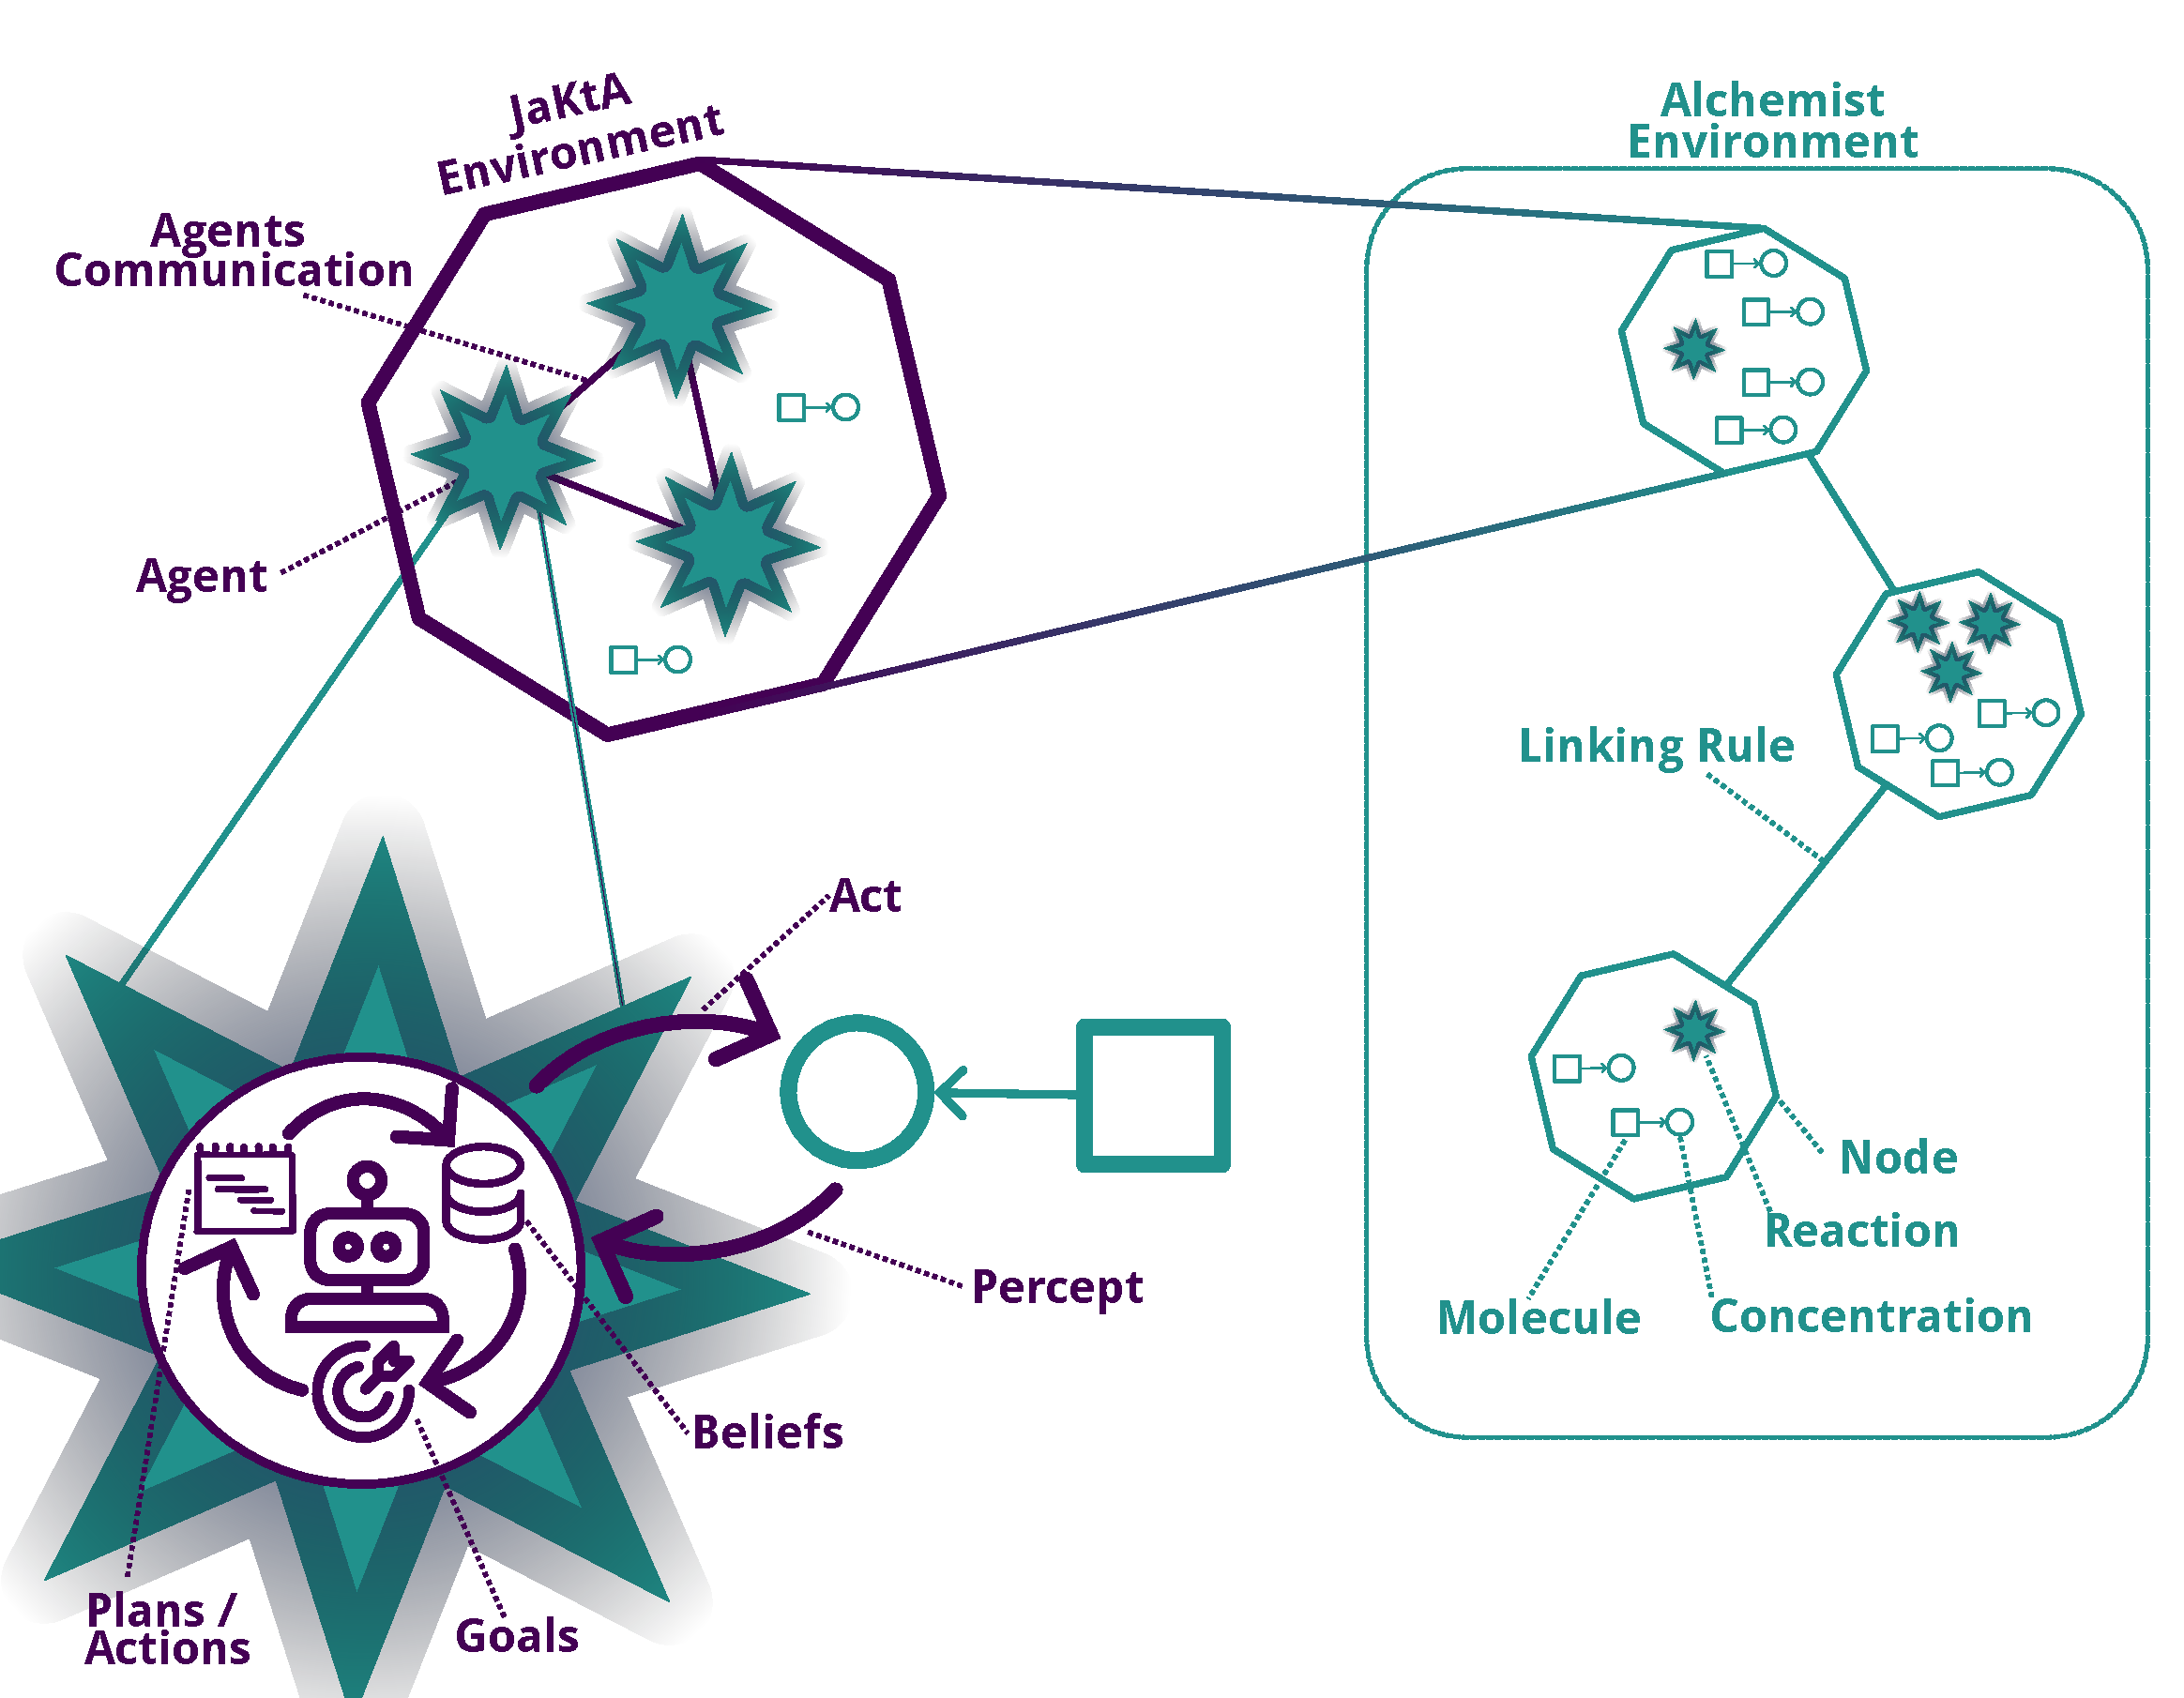
\includegraphics[width=\linewidth]{figures/jaamas26/mapping.pdf}
    \caption{
        Mapping \jakta{} BDI abstractions onto \alchemist{} ones.
        %
        Each \alchemist{} Node represents a physical \emph{device}
        running a centralised \jakta{} \ac{MAS}.
        %
        Simulation of distributed \ac{MAS} is achieved having multiple Nodes in the same environment that communicate via \alchemist{}'s Linking Rules.
        %
        Each agent's control-loop is implemented as an \alchemist{} \texttt{Reaction},
        with a custom \texttt{TimeDistribution} for each phase.
        %
        Agents can act on and perceive \alchemist{}'s molecules in the environment.
    }
    \label{fig:mapping}
\end{figure}

Integrating the two frameworks has been first an exercise of model-to-model mapping.
%
The mapping of the frameworks' abstractions on each other is summarised in \Cref{fig:mapping}.

Each agent's lifecycle phases (i.e., sense, deliberate, and act) are mapped
onto separate \ac{DES} events (\alchemist{}'s \texttt{Reaction}s).
%
As introduced in \Cref{ssec:simulation:choices},
each such event has a duration modelled through a \texttt{TimeDistribution}.
%
To guarantee that each agent's control loop phases are executed in order,
we implemented a custom \texttt{TimeDistribution}
(\texttt{JaktaTimeDistribution})
composed of three sub-\texttt{TimeDistribution}s,
one for each phase of the control loop.
%
\texttt{JaktaTimeDistribution} maintains an internal state
which tracks the current phase of the agent,
and executes the next phase according to its configured \texttt{TimeDistribution}.
%
This design allows us to flexibly support different granularities:
\begin{itemize}
    \item \ac{ACLP} is immediately and natively supported,
    as any three distributions can be picked for the three phases.
    \item To support \ac{ACLI},
    the \texttt{TimeDistribution} of the \emph{deliberate} and \emph{act} phases
    must be an as-soon-as-possible distribution
    (for instance, a negative exponential distribution with rate $\lambda=\infty$),
    thus allowing the next agent's control loop to be scheduled immediately after the previous one.
    \item To support \ac{AMA},
    in addition to the constraint used for \ac{ACLI},
    the \texttt{TimeDistribution} of the \emph{sense} phases across all agents
    must be scheduled to occur exactly once
    before any agent can execute a new control loop iteration:
    we do so by using, as \emph{sense} \texttt{TimeDistribution} for any agent,
    a \texttt{DiracComb} with a period $T$,
    starting at a random time $\tau_0 < T$.
    This strategy guarantees that every $T$ units of simulated time,
    all agents will have completed exactly one reasoning cycle,
    executed in some arbitrary (but deterministic and equal for each $T$ interval) order.
\end{itemize}

While the \texttt{TimeDistribution} for internal events depends on the chosen granularity,
external events must be explicitly modelled in the simulation configuration.
%
For example,
the movement of a \texttt{Node} in the environment is an external \texttt{Event},
thus it must be specified with its own \texttt{TimeDistribution} in the simulation.

\texttt{Node}s in \alchemist{} naturally map onto situated devices,
as they possess a defined location in space.
%
Consequently,
we could not map \jakta{}'s \texttt{Agent}s directly onto \alchemist{}'s \texttt{Node}s,
as in a distributed \ac{BDI} \ac{MAS} multiple agents can be hosted on the same device.
%
Rather,
we mapped \alchemist{}'s \texttt{Node}s into instances of devices executing the \jakta{} platform,
thus capable of hosting multiple agents at once.

Mapping \texttt{Node}s to platform instances (or devices) enables direct inheritance of the
\alchemist{}'s \texttt{Linking Rule} abstraction to model the communication channels,
and in principle allows for the implementation of mobile agents.
%
The Alchemist-compatible platform instance (named \texttt{JaktaEnvironmentForAlchemist}) is a \jakta{}-specific \texttt{NodeProperty},
adapting \jakta{} to run inside every \alchemist{} \texttt{Node},
driven by the simulator's control flow.

Agents can reason on the current device status,
as information stored inside \texttt{Nodes}'
is reified as perceived knowledge from \jakta{} agents.
%
Information inside nodes is stored as key-value pairs
(\texttt{Molecule}s) and associated \texttt{Concentration}s (c.f. \Cref{ssec:simulation:choices}),
that agents can manipulate through actions.
%
Changes are then treated by the simulator as ``regular''
environment modifications, consequent to simulated events.

Communication among agents is modeled via an \alchemist{} \texttt{NodeProperty};
each \texttt{Node} (device) is equipped with a message broker
that collects messages for the agents on that device.
%
When an agent sends a message to another agent on the same \texttt{Node},
the message is delivered directly to the recipient's message queue.
%
When the recipient is on a different \texttt{Node},
the message is delivered if the recipient's \texttt{Node} is in the neighborhood
of the sender's \texttt{Node},
according to the \texttt{LinkingRule} defined in the simulation configuration.

\section{Evaluation}\label{sec:simulation:evaluation}

In this section,
we exercise the prototype introduced in \Cref{sec:simulation:prototype}
to demonstrate \emph{feasibility} of the proposed mapping of \ac{BDI} agents over \ac{DES}
and the \emph{transparency} of execution with respect to the agent specification.
%
Additionally,
we measure the impact granularity has on the \emph{reality gap} of the simulation ($\ref{rq:des}$),
showing that the same \ac{MAS} logic can produce different emerging behaviours
when executed with different granularities.

Our evaluation mimicks a situation where
multiple \acp{UAV}, each controlled by a \ac{BDI} agent,
must cooperate to maintain a circular formation.
%
%Our team is currently lacking physical \acp{UAV},
%so we could not perform real-world experiments with actual \acp{UAV},
%yet this is perfectly fine for our purposes:
%our goal here is not really to let \ac{BDI} agents control \emph{physical} bodies
%-- that would be expensive and time-consuming --
%but rather to engineer and validate the \emph{software} of those agents via \ac{DES} simulation%
%---before \acp{UAV} are even bought.
%
%Finally,
To demonstrate the portability of the \ac{MAS} codebase
between simulation and real-world,
we show that the same code can be executed inside the simulator
or directly as a regular multithreaded application.
%
In the former case, the \ac{UAV} controls are simulated through the tools provided by the
\ac{DES} \ac{API},
while, in the latter case,
the \ac{UAV} controls are encapsulated in a different \ac{API}.

\footnotetext{
    One may argue that ``mocking'' is, in a broad sense, a form of simulation.
    %
    However,
    as we discuss extensively in \Cref{subsec:simulation:discrete-simulation},
    we consider as ``simulation'' only the execution of a system in a
    \emph{virtualised} execution environment,
    where both time and space are virtual and detached from the real world,
    and where the whole dynamic of the system is controllable.
    %
    This is not the case for mocked components.
}

It is worth highlighting that our experimental design
(specifically: the first part, where the \ac{MAS} is validated via \ac{DES})
is particularly useful to show the impact of simulation granularity onto validation.
%
In fact,
as we discuss in the next subsections,
choosing a coarser granularity for the simulation may hide potential issues in the agent programs,
which would instead emerge when a finer granularity is used.

\subsection{Use Case Description}
\label{ssec:simulation:use-case}
We use a \acp{UAV} coordination scenario as our reference.
%
We use \jakta{} to instruct a flock of \acp{UAV},
each controlled by a \ac{BDI} agent,
to build and maintain a circular formation while following a moving leader \ac{UAV}.
%
The \emph{leader} \ac{UAV} moves in a circular path (radius $r_l=5m$),
while follower \acp{UAV} must coordinate to build a circular formation around the leader
so that every follower is at distance $r_f=2.5m$ from the leader,
and all followers are equally distanced to each other.
%
This formation must be maintained while the leader moves along its path.


We assume direct \ac{LoS} \ac{UAV}-to-\ac{UAV} communication within a short range of $r_c=5m$.
%
\acp{UAV} can navigate the space at a maximum speed of $1\nicefrac{m}{s}$.
%
If no signal is received from the leader, followers hover at their current location.
%
In this scenario, we assume \acp{UAV} are equipped with some localisation system that provides them with exact coordinates of their position in a given shared reference system.
%
Initially,
follower \acp{UAV} are randomly displaced into a circular arena of radius $10m$,
while the leader is located at the arena centre.

Each \ac{UAV} runs the \ac{BDI} control loop in rounds
at a certain maximum execution frequency
$f = \nicefrac{1}{T}$, cf. \Cref{subsec:simulation:mapping}.
%
Each control-loop phase would take some time to complete, depending on the complexity of the computations involved.
%
For instance, a frequency of $f=1Hz$ implies the execution
    of one agent control loop per second.
Tuning this frequency is a way to balance the responsiveness of the agent to changes in the
    environment with resource utilization (e.g., battery consumption),
and must be tuned to stay within the physical limits of the \ac{UAV}'s hardware.

Additionally,
devices are not started simultaneously,
each of them experiences a random start delay $\tau_0 \in [0, \nicefrac{1}{f}]$
    (or, equivalently, $\tau_0 \in [0, T]$ see \Cref{subsec:simulation:mapping}).

\subsection{Modeling \ac{UAV} Behaviour in \jakta{}}
\label{ssec:bdi-behaviour}

During the experiment we deliberately used simplified \ac{BDI} programs that rely on tight synchronisation of agents' control loops.
%
We model two agent roles: a single \emph{leader} and multiple \emph{followers}.
%
The leader continuously traverses a circular trajectory at constant speed.
%
Its behaviour is expressed as a single \ac{BDI} goal named \texttt{move}
(i.e., following the circular path)
and an associated plan that repeatedly:
\begin{enumerate}
    \item moves the leader to the next waypoint along the circle, and
    \item broadcasts a message to nearby agents (within communication radius $r_c$) inviting them to join the formation.
\end{enumerate}
%
Followers do not possess a proactive goal;
they are reactive agents driven by messages from the leader.
%
Upon receiving a ``join formation'' message,
a follower executes a plan that computes and moves to its assigned position in the circular formation.
%
The target position is determined from the current number
of followers already in the formation.
%
The \ac{BDI} program that expresses this behaviour is shown in \Cref{fig:code}.

\subsection{Experimental Setup}
\label{ssec:experimental-setup}
Given the shared behavior implementation described above,
in this section we describe how we experimented with the developed prototype
to demonstrate that:
\begin{itemize}
    \item different granularities in the simulation execution may lead to different emergent behaviours of the \ac{MAS},
    \item the same \ac{MAS} codebase can be executed both in simulation and on a real-world deployment without modification.
\end{itemize}

\acp{UAV} in a real system would run independently.
This makes the \ac{ACLP} granularity the most realistic one,
as it allows for control-loop phase interleaving.
%
Simulating at a coarser granularity
may lead to incorrect forecasts about the correctness of the agent program.

To demonstrate the portability of the \ac{MAS} codebase to a real-world deployment,
we execute the \ac{UAV} control \ac{MAS} as a regular process
where all agents run concurrently as threads.
%
This is, of course,
a simplified approximation of a deployment on real \acp{UAV},
but it suffices to show that the same codebase can be executed
without modification in both simulation and real-world settings.

We ensured code portability
by enforcing that all interactions with the environment are done through the \jakta{} environment \ac{API},
which we implemented both for the real-world deployment and for the \alchemist{} simulator.

\subsubsection{Simulated System Deployment on the \alchemist{} Simulator}
\label{ssec:simulator-execution}

We use the simulator to compare the execution of the same \ac{MAS} logic
with different granularities, namely,
    we consider \ac{AMA}, \ac{ACLI}, and \ac{ACLP} (cf. \Cref{ssec:simulation:granularity}).
%
We expect that coarser-grained granularities show better system performance
than more finer-grained
(in our case, better formation maintenance).
The experiment is designed to show that such effect is 
a consequence of the over-simplification of the \ac{BDI} program
and of its execution using coarse-grained simulation.
% It turns out that,
% when simulating coarse-grained granularity levels
% (namely, \ac{AMA} and \ac{ACLI})
% the agents are able to maintain the formation,
% while the fine-grained \ac{ACLP} granularity level reveals
% that this result is an artefact of
% the over-simplification of the \ac{BDI} programs.
% %
% On a real \ac{UAV}-programming workflow,
% this would have revealed a flaw in the agent program,
% or highlighted the need for higher responsiveness
%     (reasoning cycle frequency)
% to react to the dynamics of the environment.
%
%Should the engineering workflow be a real one,
%this is where engineers would go back and write better \ac{BDI} programs.
%%
%But,
%for the sake of our evaluation,
%this is sufficient to show how simulation can be used to validate \ac{BDI} agents' behaviour,
%and how the granularity of the simulation impacts the quality of the analysis.

\paragraph{Modeling \acp{UAV}}

\acp{UAV} are modelled as \alchemist{} \texttt{Node}s.
Each \texttt{Node} is mapped to a \jakta{} platform instance
that hosts a single \jakta{} agent controlling the \ac{UAV} as described in \Cref{subsec:simulation:mapping}.

Nodes can move in a 2D continuous space using the \alchemist{}'s built-in \texttt{MoveToTarget} action. Agents compute the desired destination based on the perceived positions of the other \acp{UAV} and the leader, and write it to a dedicated \texttt{Molecule} in the environment, which is then read by the \texttt{MoveToTarget} action during its execution which applies the movement considering a speed parameter.
%
This mechanism is used to make movement realistic and not instantaneous in the simulation, as \acp{UAV} can only move at a maximum speed of $1\nicefrac{m}{s}$.

A pictorial representation of the experiment in form of simulation snapshots is shown in \Cref{fig:graphical-behaviour}.
%
For the sake of conciseness,
we do not provide the complete \ac{MAS} code here,
but we highlight in \Cref{fig:code} the platform-agnostic specification and how it is bound with the
underlying execution platform.
%
We refer the interested reader to the companion artefact~\cite{zenodojaktajaamas}
available online\footnotemark for the complete codebase of the experiment.


\begin{figure}
    \begin{minipage}[b]{.62\linewidth}
        \centering
        \lstinputlisting[
            language=Kotlin,
            linewidth=\linewidth,
            basicstyle=\scriptsize\ttfamily,
            label={lst:logic},
    %        caption={Platform-agnostic code}
        ]{listings/jaamas26/agentsLogic.kt}
    \end{minipage}\hfill
    \begin{minipage}[b]{.34\linewidth}
        \centering
        \lstinputlisting[
            language=Kotlin,
            linewidth=\linewidth,
            basicstyle=\scriptsize\ttfamily,
%        caption={Entrypoint},
            label={lst:agents}
        ]{listings/jaamas26/agents.kt}
    \end{minipage}
    \caption{
        Code extracts from the companion artifact.
        The agent specification (left) is completely platform-agnostic and reusable,
        some glue code (right) wires the logics with the underlying execution platform.
    }
    \label{fig:code}
\end{figure}

\begin{figure*}
    \centering
    
\includegraphics[width=.32\linewidth]{figures/jaamas26/optimal_behaviour.png}
    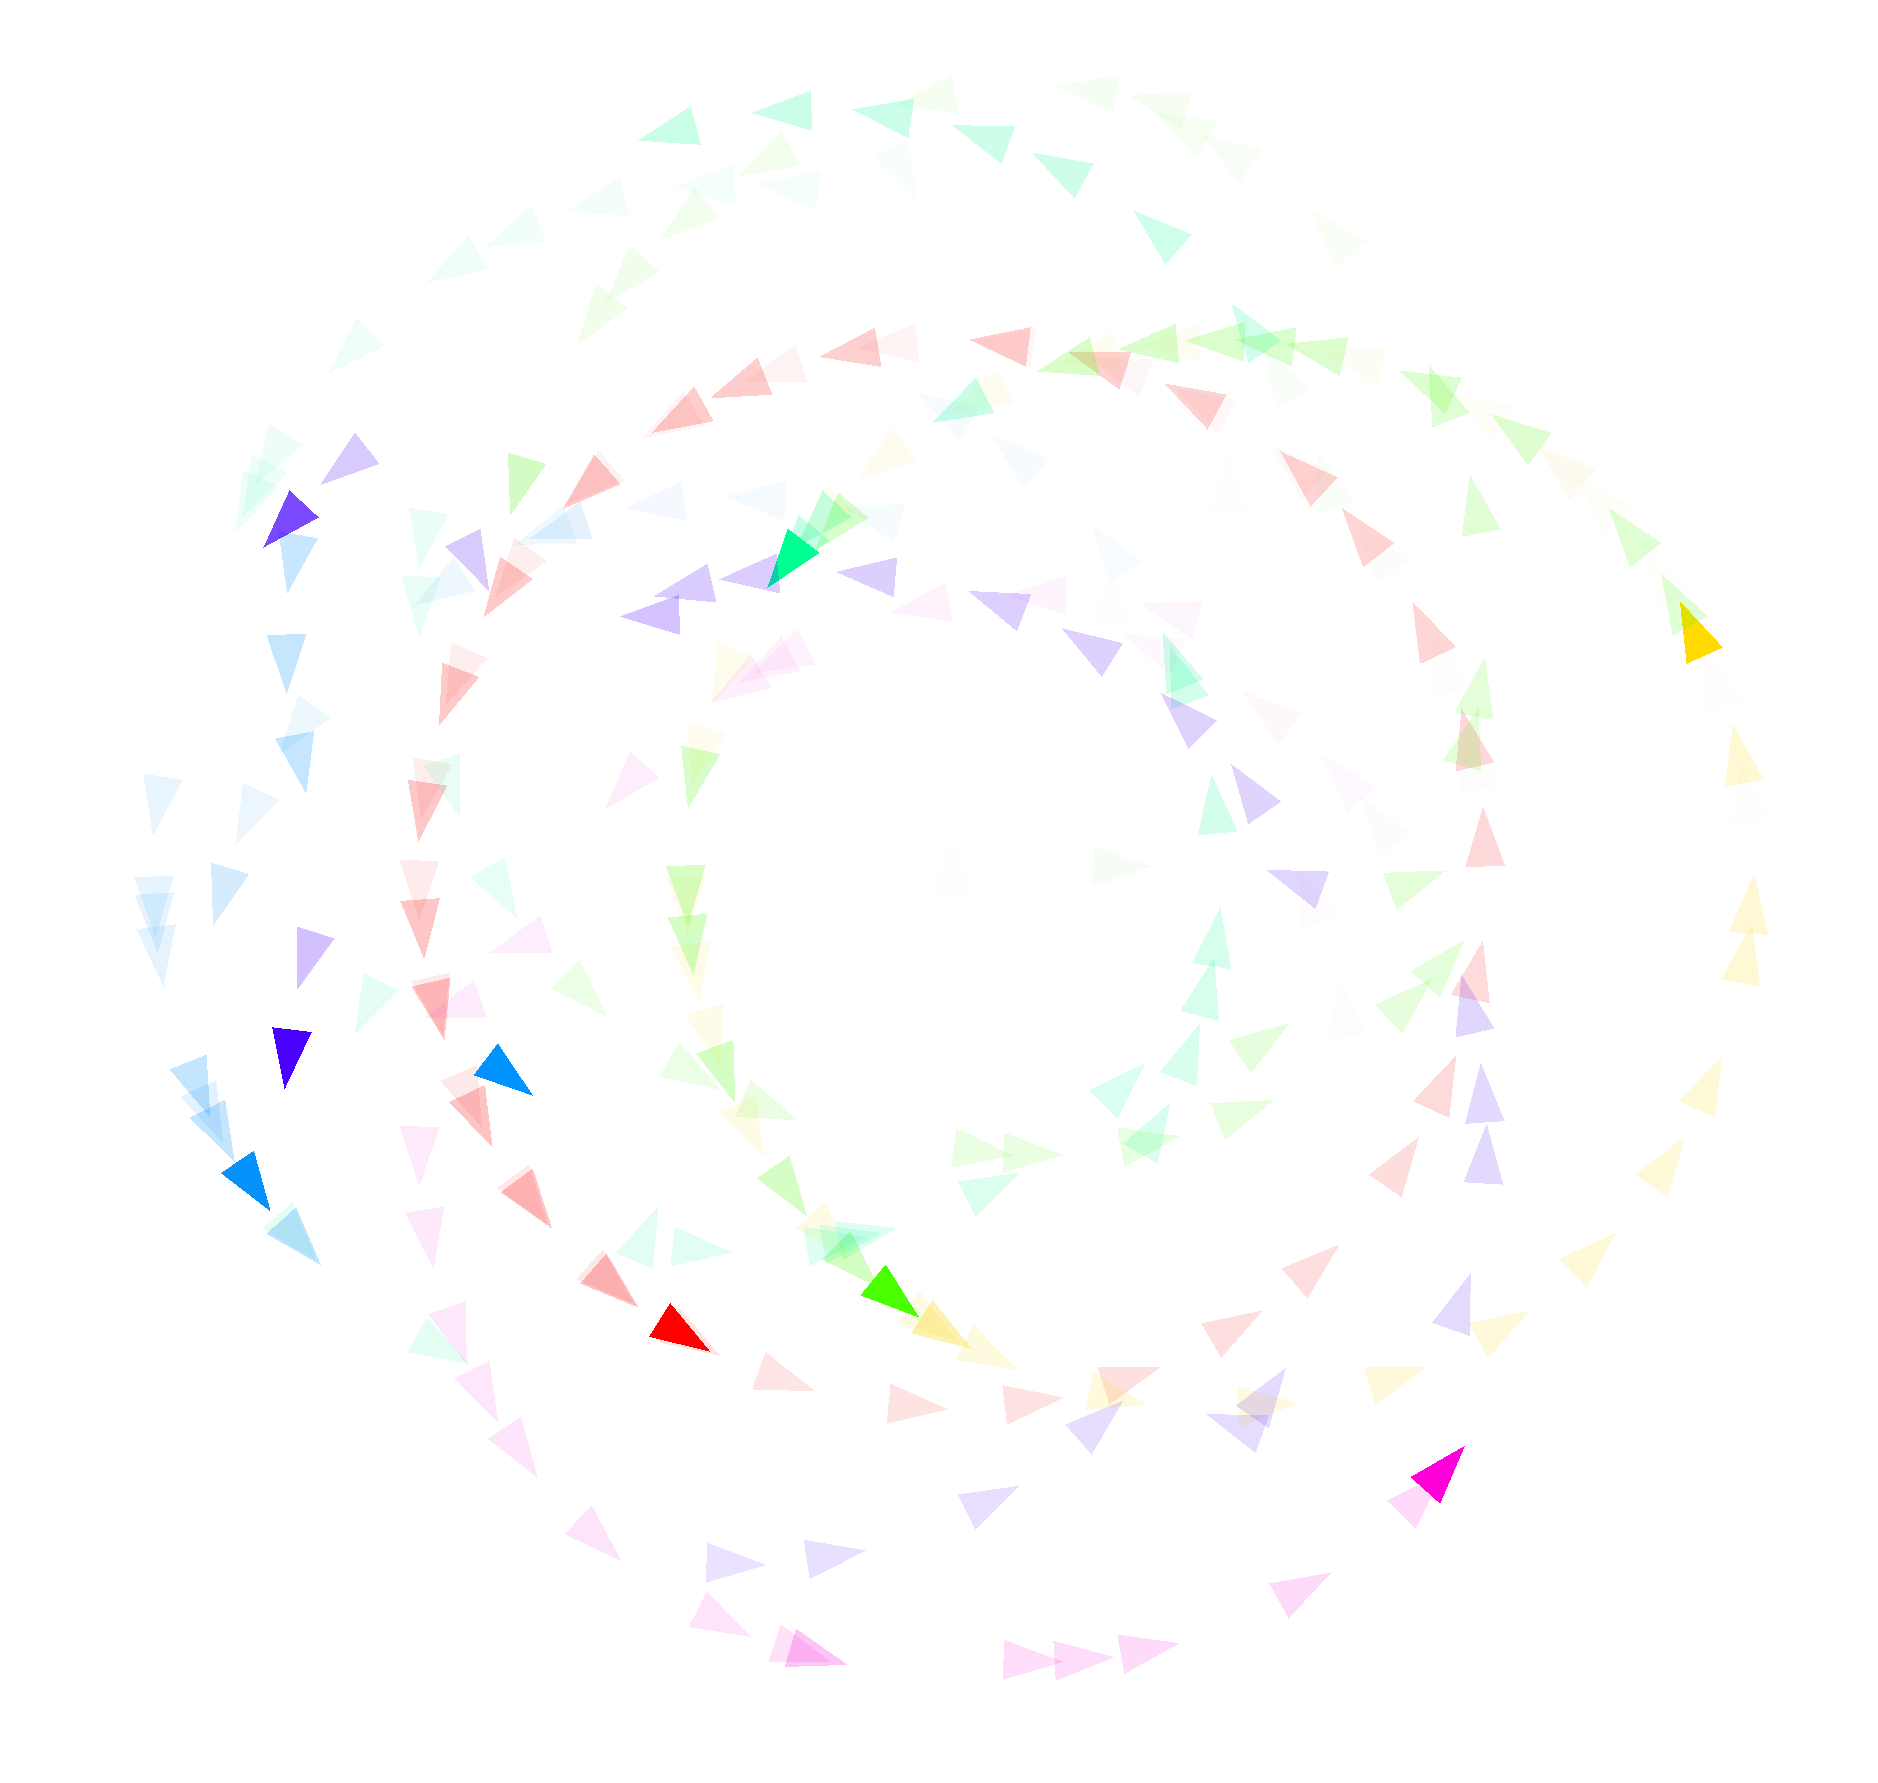
\includegraphics[width=.32\linewidth]{figures/jaamas26/delayed_behaviour.png}
    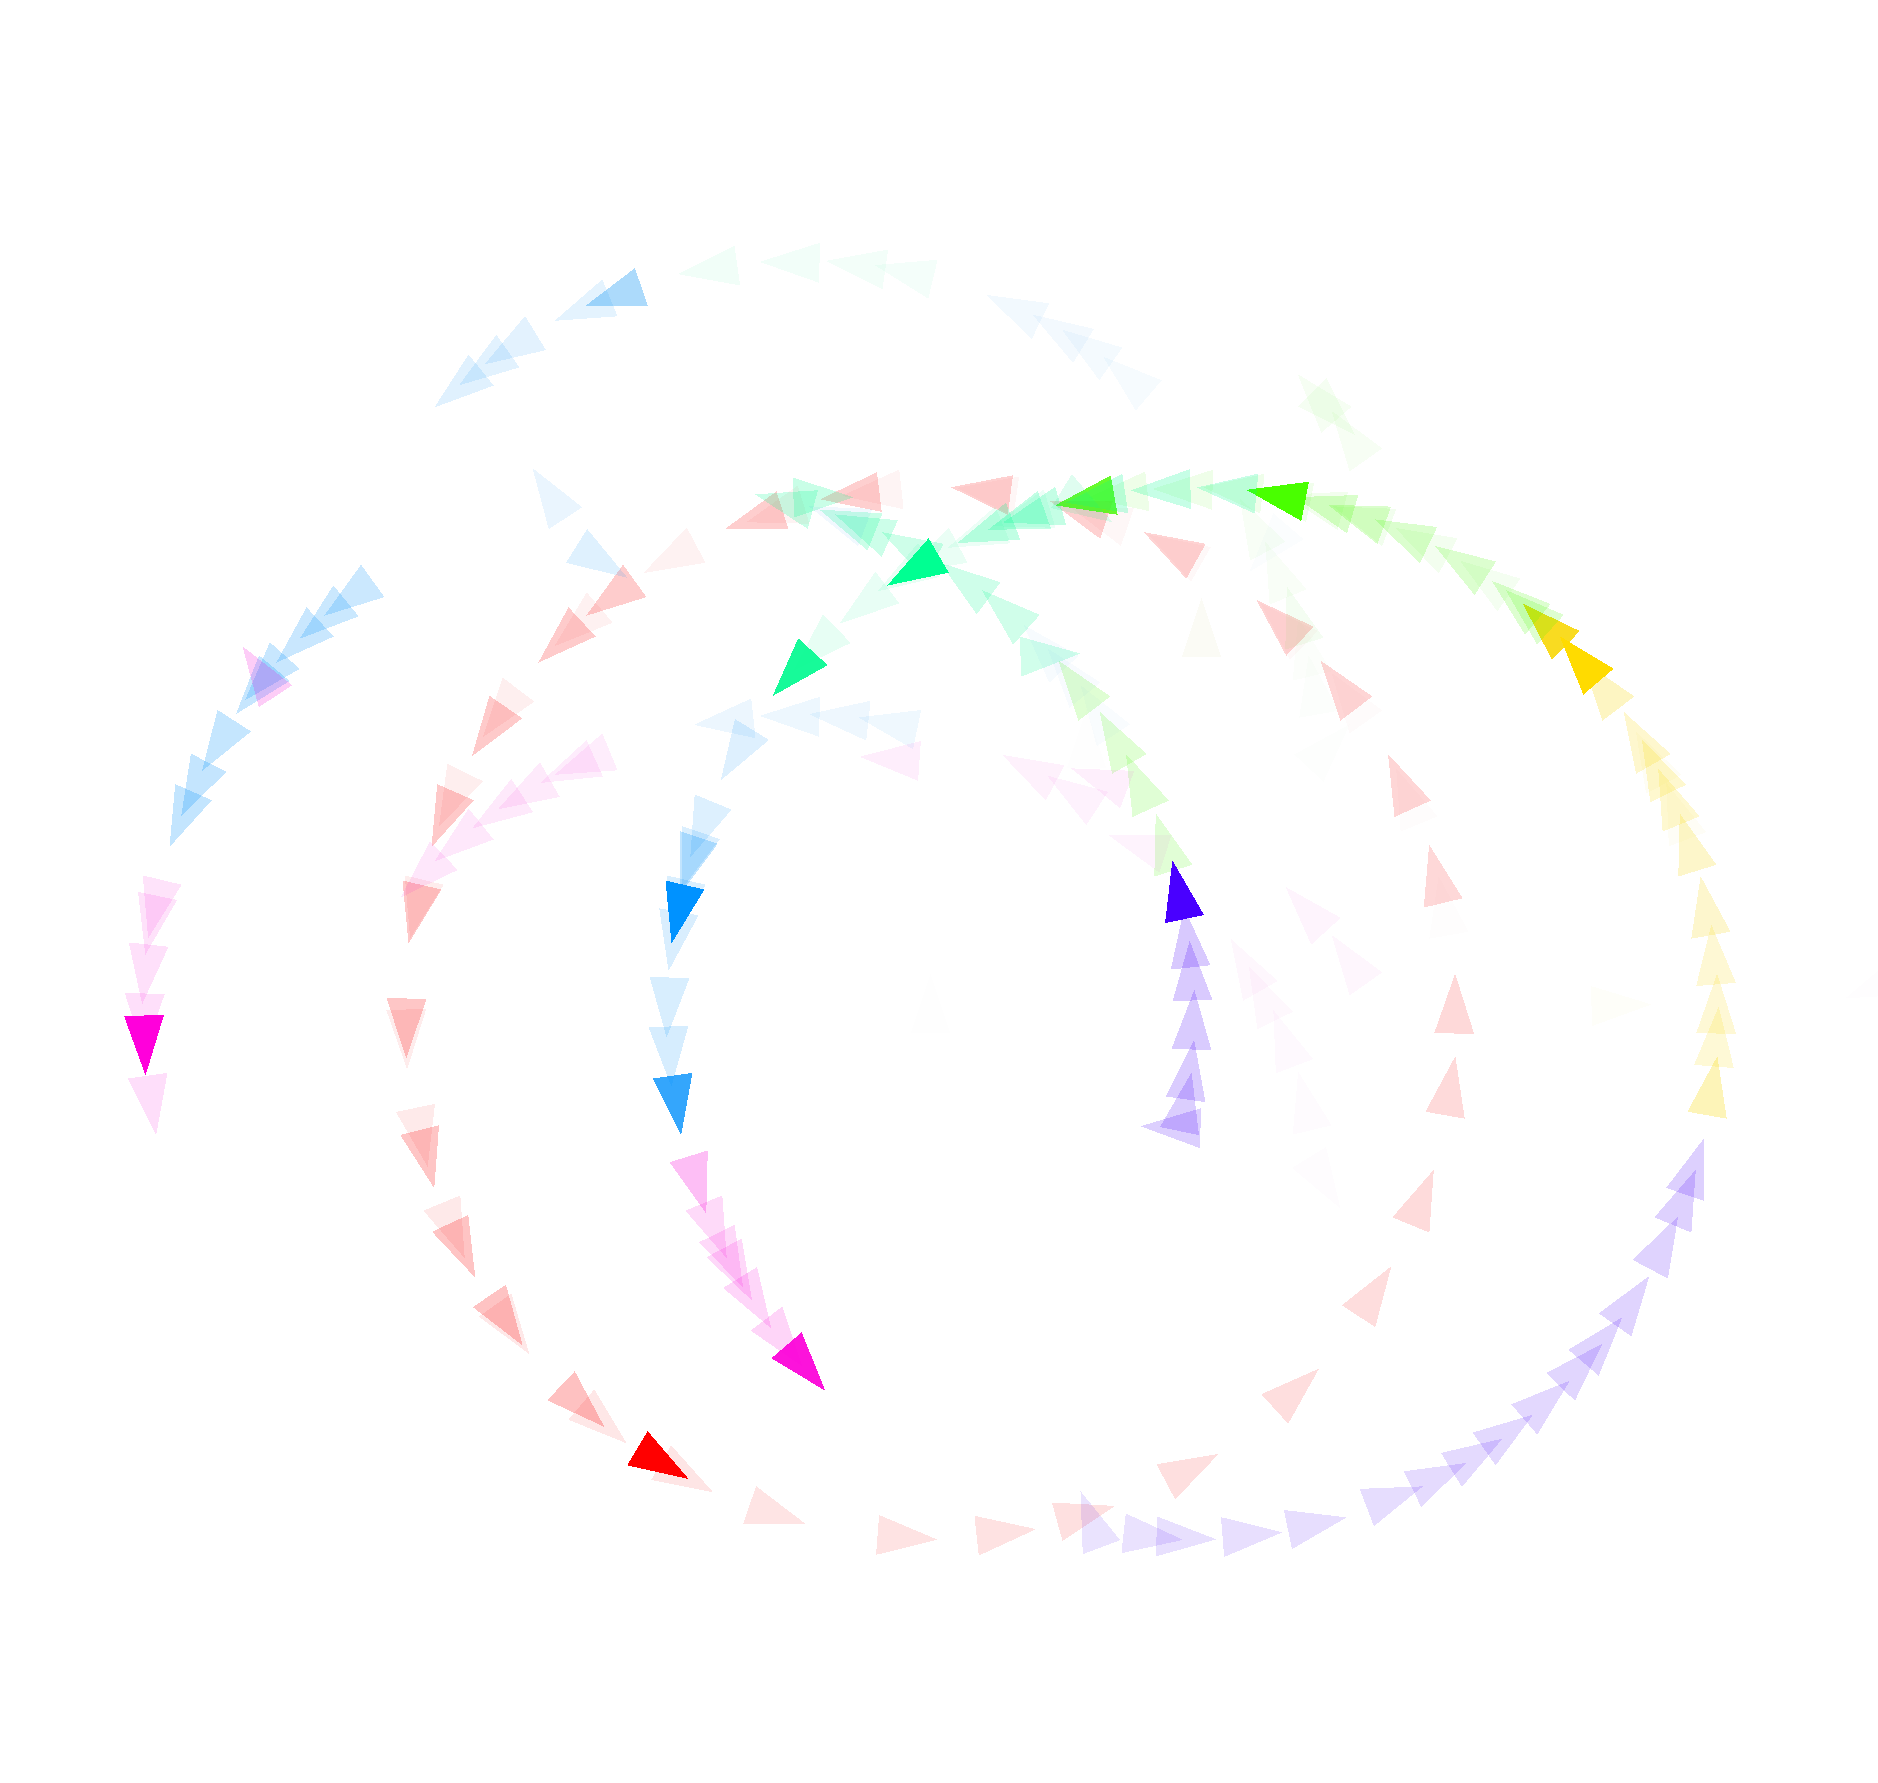
\includegraphics[width=.32\linewidth]{figures/jaamas26/destroyed_behaviour.png}
    \caption{
        Simulation snapshots for the three cases: \ac{AMA} (left), \ac{ACLI} (centre), and \ac{ACLP} right
        for $\tau=0.6$.
        Every \ac{UAV} is depicted with a different colour, the leader is the red one.
        The follower \ac{UAV} count has been reduced to six for better visualisation.
        Color intensity captures the distance in time, more intense colors are closer to the current time.
        In \ac{AMA}, all \acp{UAV} follow a circular trajectory intersecting the leader's one.
        The formation is much less regular in \ac{ACLI}, and it is completely lost in \ac{ACLP},
        showing that failing to capture the model nuances correctly may produce systems that work
        \emph{because} of the abstraction gap.
    }
    \label{fig:graphical-behaviour}
\end{figure*}

\paragraph{Configuring the Agent Execution and Simulation Parameters}

We investigate how the mapping granularity (cf. \Cref{ssec:simulation:granularity}) impacts the system's behaviour.
%
To do so, we use \ac{AMA} as baseline,
letting the entire \ac{MAS} run a full cycle every simulated second
(Dirac Comb distribution with frequency $f=1Hz \rightarrow T=1s$, cf. \Cref{subsec:simulation:mapping}),
thus replicating the behaviour of most current agent-based simulation frameworks, which are time-driven.
%
We compare the baseline with \ac{ACLI} and \ac{ACLP},
for which, however, we model
each agent's control-loop frequency following a Weibull distribution with mean $f$ and deviation $f\cdot\tau$ (drift).
%
Intuitively, this means that most loops will be scheduled around the mean frequency $f$, but some loops will be scheduled earlier or later, thus introducing a drift $\tau$ in the agents' execution.

Additionally, for the \ac{ACLP} granularity we model deliberation and action delays,
associating each phase with an exponential distribution with rate $\lambda = f$:
faster agents (larger $f$ values) have less delay.
%
This is needed to emulate a real-world concurrent deployment, in which different phases of the control loop may take different time to complete and may interleave.

Every experiment is repeated $100$ times with a different random seed, changing
the initial positions of the followers
and the distribution in time of the events for the \ac{ACLI} and \ac{ACLP}.
%
In each experiment, the leader follows a circular trajectory of radius $r_l=5m$
and is set to complete a full circle in $600s$.
%
We let the system execute for $1500$ simulated seconds.



\subsubsection{Real-World System Deployment as a Concurrent System}
\label{ssec:real-world-execution}

To demonstrate the seamless execution of the same \ac{MAS}
specification in both simulated and real systems,
we run the \jakta{} \ac{MAS} natively on a stand-alone desktop computer.
%
The execution model in \jakta{} runs each agent in a separate thread,
thereby emulating a concurrent deployment on independent \acp{UAV}.

In this setup,
\acp{UAV} run at the maximum allowed frequency $f$,
determined by the host machine's CPU capabilities.
%
Any relative drift $\tau$ between different \acp{UAV}
is naturally introduced by the operating system's scheduler.
%
The duration of each phase of the control loop depends
on the actual computation time of the agent program,
which in turn is determined by the host machine's CPU performance.

Agents interact with a local instance of the environment
implemented as a specialization of the generic \jakta{} \texttt{Environment}
(cf.~\Cref{par:jakta}).
%
The environment is responsible for emulating the \acp{UAV}' physical aspects,
such as position and communication.

Concerning communication between \acp{UAV},
agents exchange messages via the environment:
each agent invokes the broadcast primitive provided by the environment,
which delivers the message to all agents whose current
positions lie within the sender's communication radius $r_c=5m$.
%
Concerning positioning,
the environment stores \acp{UAV} positions as two-dimensional coordinates.
%
When an agent attempts perceiving its own position,
the environment returns the stored coordinates.
%
When an agent attempts to move to a target destination,
it sends a request to the environment,
which in turns stores that desired destination for that agent.
%
The actual movement is completed asynchronously via a co-routine which runs in background.
%
This co-routine would periodically (as frequently as possible) update the positions of each \ac{UAV}
along the straight line toward its target destination,
by a distance non-greater than $1m$
(so that $v_{\max}=1\nicefrac{m}{s}$).

This setup demonstrates the portability of the \ac{MAS}
codebase to a non-simulated deployment:
the same code used in simulation runs unchanged here.
%
The experiment\footnotemark[\value{footnote}]
shows the identical codebase executed in both simulated and real-world settings.
%
%    In simulation we run
%    \texttt{it.unibo.jakta.examples.simulation.LeaderDrone} and
%    \texttt{it.unibo.jakta.examples.simulation.FollowerDrone};
%    in the real-world deployment we run
%    \texttt{it.unibo.jakta.examples.main.LeaderDrone} and
%    \texttt{it.unibo.jakta.examples.main.FollowerDrone}.
%
The experiment was executed on a machine with an Intel i7-10750H CPU (2.60 GHz) and 32 GB RAM\@.

%
\footnotetext{
    \url{https://github.com/anitvam/uav-circle-2024-jakta-alchemist}
}

\subsection{Results}
\label{ssec:results}

In this section we present and discuss the results of our experiments,
focusing on the impact of the simulation granularity on the system behaviour.
%
We discuss the results obtained when simulating the system first,
then we present the results obtained from the concurrent system execution.

We evaluate the system performance by measuring the deviation from the ideal positions.
%
More precisely,
we use an oracle to determine the ideal position of each follower based on the current leader's position,
then,
for each follower $u$,
we measure the distance error $d_u$ between the ideal and actual position of $u$.
%
% Provided these distances,
% for all followers $u \in U$
Our error metric is the overall
squared distance error:
%sum of squares of the distance errors of each follower:
$\sum_{u \in U} d_u^2$.


Results confirm the expectations that
when simulating coarse-grained granularity levels
(namely, \ac{AMA} and \ac{ACLI})
the agents are able to maintain the formation,
while the fine-grained \ac{ACLP} granularity level reveals
that this result is an artefact of
the over-simplification of the \ac{BDI} programs.
%
On a real \ac{UAV}-programming workflow,
this would have revealed a flaw in the agent program,
or highlighted the need for higher responsiveness
    (reasoning cycle frequency)
to react to the dynamics of the environment.


\subsubsection{Analysis of the \alchemist{} Simulated System Deployment}

\begin{figure*}
    \centering
    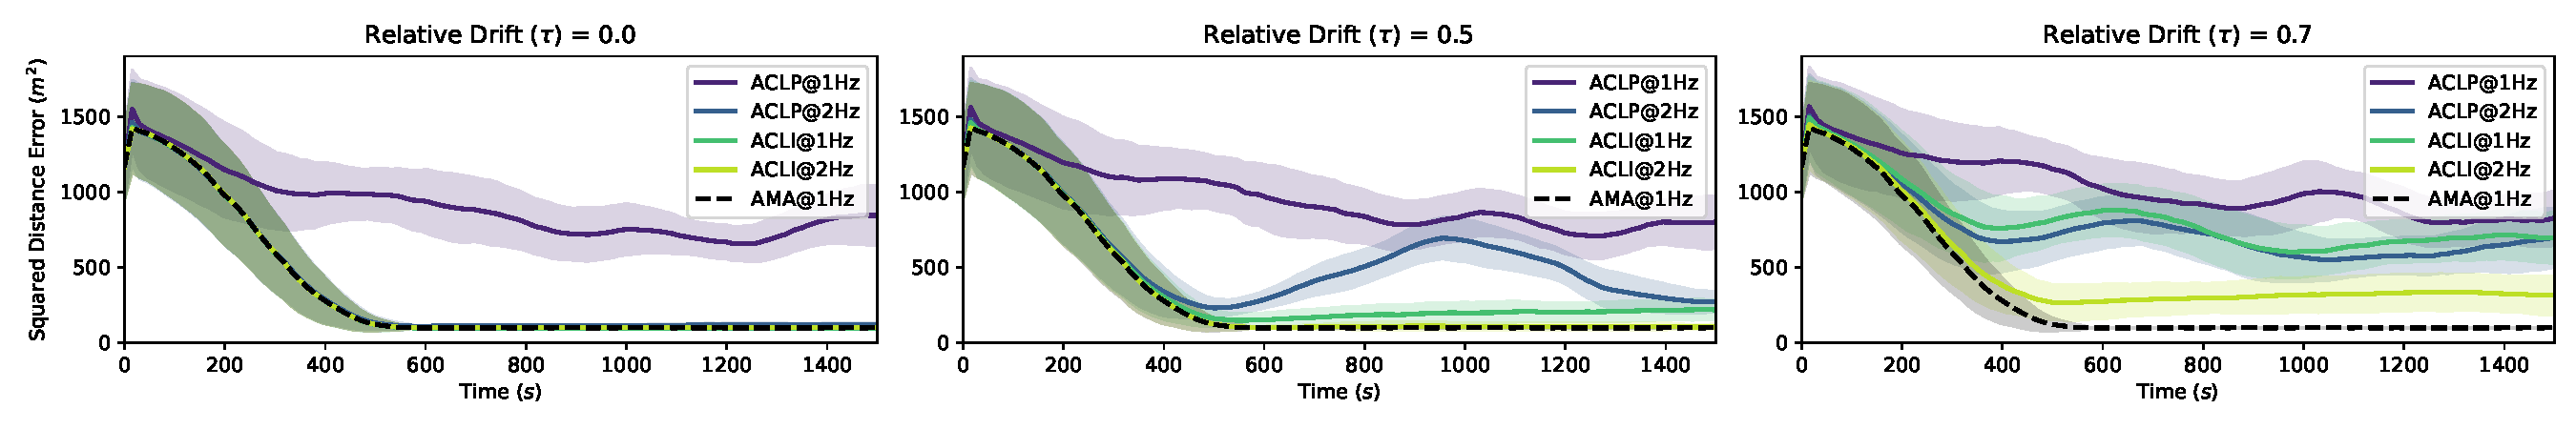
\includegraphics[width=\linewidth]{figures/jaamas26/error_over_time_flattened.pdf}
    \caption{
        Error with time for different granularities, with \ac{ACLI} and \ac{ACLP} running at $f=1Hz$ and $f=2Hz$.
        Different charts show different values of relative drift $\tau$.
        Coloured shadows represent $\pm 1\sigma$.
    }
    \label{subfig:err_time}
\end{figure*}
%
\begin{figure*}
    \centering
    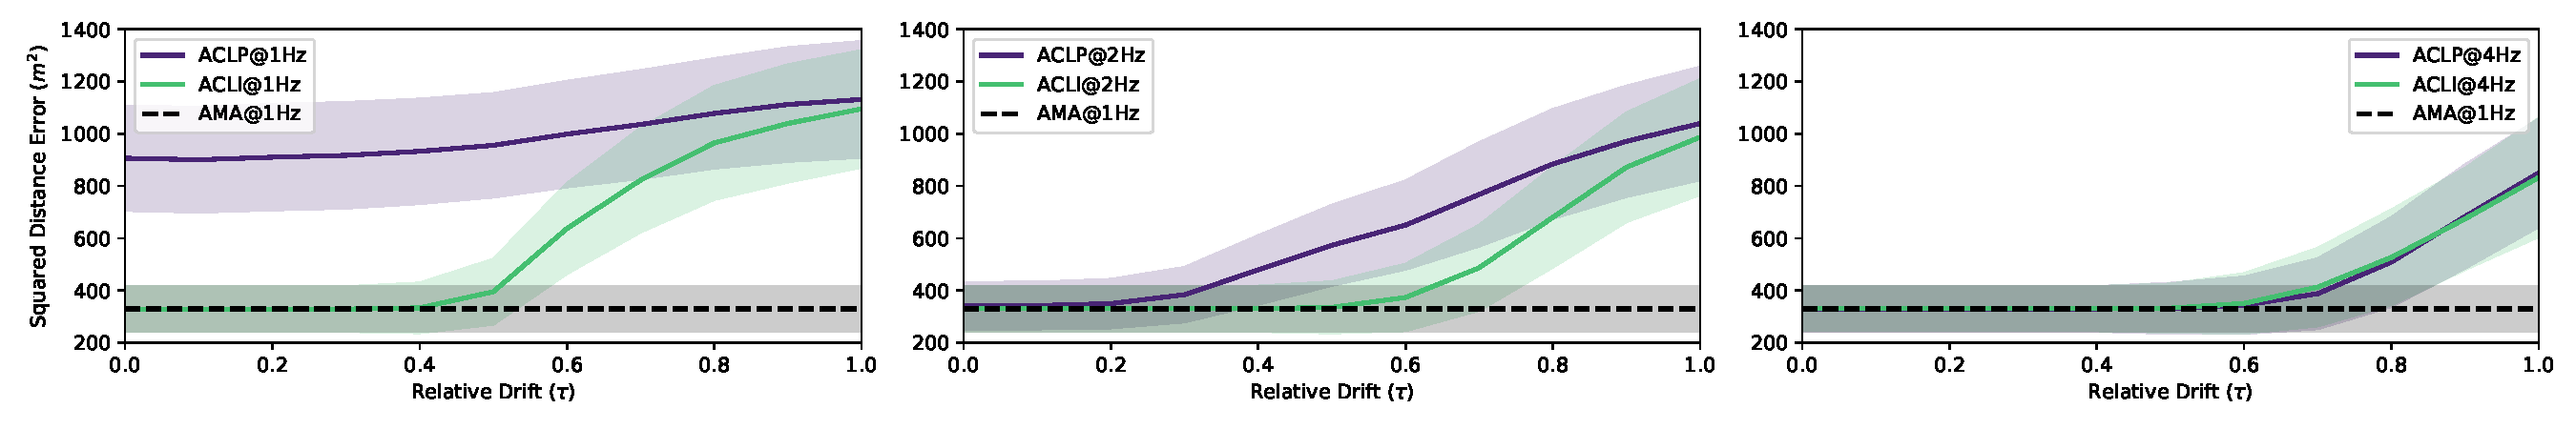
\includegraphics[width=\linewidth]{figures/jaamas26/error_over_variances.pdf}
    \caption{
        Mean squared distance error with relative drift ($\tau$), measured for different frequencies for \ac{ACLI} and \ac{ACLP}.
        Coloured shadows represent $\pm 1\sigma$.
    }
    \label{subfig:err_drift}
\end{figure*}

\Cref{subfig:err_time} shows the evolution in time results for $\tau \in \{0, 0.5, 0.7\}$.
%
With \ac{AMA} granularity,
after a transient phase in which the leader is still contacting the followers,
the error stabilises to a very low level,
due to the natural delay between the commands issued by the agent execution
and their realisation by the \ac{UAV}.
%
When $\tau=0$, \ac{ACLI} shows the same behaviour for both $f=1Hz$ and $f=2Hz$:
the system can apparently cope with the problem at hand.
%
%Interestingly,
As expected, given that the simplistic agent logic we implemented relies on implicit synchronisation,
when using the most fine-grained model (\ac{ACLP}),
which is capable of modelling delays between one agent phase and another,
%we discover something different: the error is much larger than expected, indeed,
the simulation reveals that the error compared to the ideal positions is much larger.
Indeed,
the system seems to be able to cope with the problem at hand only when the agent runs at $2Hz$:
we have thus evidence that there are cases in which capturing a finer grained model
can provide insights
on the system's behaviour
that are not visible with a coarser granularity,
potentially imposing additional design or deployment constraints
(in this case, we must execute at at least $2Hz$ if we want the system to be robust to delays).

This result is important:
since the \acp{UAV} in the target deployment would run independently,
the \ac{ACLP} granularity is the most realistic one.
%
If the developers had simulated the system with \ac{ACLI}
(or, worse, \ac{AMA}) granularity,
the system would have failed when deployed,
despite positive feedback from the simulation.


If we introduce relative drift in the agent's execution frequency
-- thus improving the realism of the simulation --,
we can observe errors even with the \ac{ACLI} model.
%
With $\tau=0.5$, both \ac{ACLI} and \ac{ACLP} show that the system can work reasonably well, but only with $f=2Hz$.
%
Raising $\tau$ further shows that capturing the agent phases is relevant,
as the performance of \ac{ACLI} and \ac{ACLP} differs also for $f=2Hz$.

The impact of $\tau$ on the system is better evidenced in \Cref{subfig:err_drift},
where we sample multiple values of $\tau$ for different $f$.
%
We
%learn
demonstrate that the \ac{ACLI} model provides unreliable results at lower frequencies,
while it is comparable to \ac{ACLP} as the frequency increases.
When the system is challenged, and the frequency is barely insufficient to cope with the problem,
it tends to provide overly optimistic results,
thus making the system appear as working as intended when, with better detail, we can observe that it is not.
%
Designers can use this information to decide whether their software needs to be amended,
or they may clearly state that it is required for the target \ac{UAV} to be capable to run the agent software
at a minimum frequency.

\subsubsection{Analysis of the Real-World Concurrent System Deployment}
\label{sub-ssec:concurrent-results}
    The execution of the same \ac{MAS} logic on a concurrent system
    produced results comparable to those obtained in simulation at the \ac{ACLP} granularity,
    demonstrating that simulation granularity affects the system's evaluation.
    %
    The error metric for the concurrent-system execution was measured once per second,
    and the outcome is shown in \Cref{fig:real-world-error}.

    In line with expectations,
    the error follows the \ac{ACLP} simulation results,
    confirming that coarser-grained event granularities in simulation
    may obscure subtle concurrency-dependent effects.
    %
    This is confirmed by results shown in \Cref{fig:real-world-error},
    where the error does not stabilise or decrease towards zero,
    which is instead the behaviour we would expect from a correct system.

\begin{figure}
    \centering
    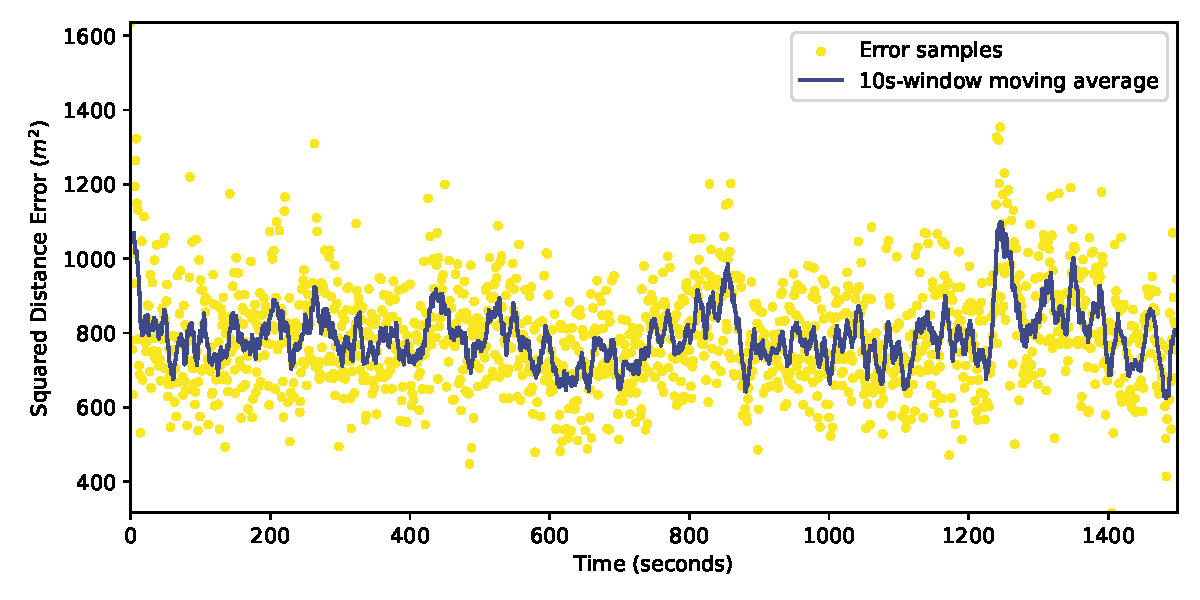
\includegraphics[width=\linewidth]{figures/jaamas26/main_execution_line_chart.pdf}
    \caption{
        Error over time for the execution of the \ac{BDI} \ac{MAS} on a concurrent system.
        Yellow line represents the raw error measurements,
        gathered once every second.
        Blue line is the rolling average over a window of $10s$.
    }
    \label{fig:real-world-error}
\end{figure}

\subsubsection{Discussion}

With this experiment, we demonstrated that
the execution of a \ac{BDI} \ac{MAS} in a \ac{DES} is \emph{feasible}
and can be realised at different granularity.
%
We also show that the \ac{BDI} code
can be ported \emph{transparently} into the simulation environment,
as it does not directly refer any simulator- or platform-specific entity.
%
\Cref{fig:code} shows that the code of \ac{BDI} specification (left) is completely agnostic of the final destination of the agent
and programmed using pure \jakta{} syntax,
that can run both in a simulation and in a real-world scenario,
provided that the necessary interactions with the environment
(e.g., the action \texttt{circleMovementStep}) are appropriately modelled in both settings.
%
Finally, we show that the impact of the chosen granularity on the \emph{reality gap} is a relevant issue
and that executing a \ac{MAS} in modes that induce \emph{implicit synchronisation}
(\ac{AMA}, and, to a lesser extent, \ac{ACLI})
can produce unreliable results,
especially concerning the system's performance.

The example highlights
how simulating the \ac{MAS} behaviour before deployment
can be a valuable tool for software engineers,
allowing to identify potential issues.
%
In this case, the simulation provides insights
on the relative frequency agents need to run to cope with the problem.
Having observed that the system may fail under certain conditions,
the developers of the agent specification may decide to introduce additional mechanisms
to improve the system's reliability.

\section{Threats to validity}
\label{sec:limitations}
% \samu{R3 dice che non si capisce se la simulazione è utile oppure no. Cambiando esempio sicuramente possiamo migliorare questo punto ma forse possiamo dire qualcosa in più anche qui}

% \samu{Porterei la discussion a livello di section assestante e discuterei più nel profondo le limitazioni correnti dell'approccio e del prototipo, e come si potrebbero superare. Discuterei la generalità del metodo proposto, come si potrebbe applicare ad altre tecnologie, e perché non facciamo un comparison con gli altri approcci in letteratura (cose che abbiamo scritto nel rebuttal). Idem si possono commentare scalabilità ecc. Anche una discussione legata all'effort chiesot ad uno sviluppatore per fare il porting sul MAS come chiesto da R3 ha senso.}

Here we briefly comment on a few critical aspects of our study design,
which may appear as threats to the general validity of the proposed approach.
We motivate design choices, and discuss how specific threats have been mitigated,
or why they have been accepted for the current work
with the plan of addressing them in future research.

\paragraph{Specificity of technological choices}

Our prototype is tailored on \jakta{} and \alchemist{},
which are technologies which have been designed and developed by some authors of this paper.
%
While this can be seen as a threat to the generalization of our results,
we argue that addressing our research questions
is also a technological task,
which requires technological commitments.
%
While we try to keep the conceptual discussion about the mapping
(\Cref{sec:simulation:bdi-over-des})
as general as possible,
we preferred to rely on technologies we know well when implementing the mapping.

Furthermore,
the technological affinities between \jakta{} and \alchemist{},
were key enablers for the development of this research line,
and this is yet another reason why we chose them.

\paragraph{Comparisons with other methods}

We deliberately avoid comparisons with other approaches for \ac{BDI} simulation.
%
The reason behind that is that,
as discussed in \Cref{sec:simulation:related-works},
we are not aware of any prior attempt to run \ac{BDI} \acp{MAS} on \acp{DES}
with the same level of granularity we propose
and comparisons with other approaches would be unfair.
%
As the existing frameworks for \ac{BDI} simulation are mainly based on \ac{DTS},
we detailed conceptual differences with \ac{DTS} frameworks.
%
Yet,
we could not see the benefits of benchmarking our approach against other approaches based on \ac{DTS}.
%
In particular,
we expect \ac{DTS} would serve as a good engineering tool too,
despite being less adequate to study the effect of simulation granularity on the \ac{BDI} engineering process.

\paragraph{Performance analysis}

We do not study our solution from a computational complexity perspective,
and we do not investigate the performance of the simulation.

At the conceptual level,
our goal is to study the impact of simulations in the validation of \ac{BDI} systems,
and the role of \ac{DES} in this process.
%
We take an angle which is rooted in software engineering,
so we are more interested in studying what \ac{BDI} engineers can do with simulations,
rather than how fast the simulations run.
%
That said,
in our framework,
the computational cost of simulations is straightforward to estimate qualitatively:
fine-grained granularity levels will be more computationally expensive than coarse-grained ones,
as they require more events to be simulated.

Other practical considerations about performance are actually inherited to the technological choices we made.
%
\jakta{} is a lightweight \ac{BDI} framework,
still in its infancy,
but under active development,
and performance analysis are part of the roadmap.
%
\alchemist{} is a mature \ac{DES} framework,
which has been used in the past to simulate large-scale systems,
as proved by the many publications that rely on it for their experiments.
%
So,
in this work,
performance is not a concern,
and not even a controllable variable.

\paragraph{Effort required to design and run a testing scenario}

The byproduct of our feasibility study is a prototype tool
that may be interesting for the community of \ac{BDI} developers.
%
Despite the usability of the tool is not the focus of this paper,
we understand that it might be interesting to evaluate it
to understand how easy it is to run a \ac{BDI} simulation via \jakta{}+\alchemist{}.
%
We consider refining and evaluating the usability of the tool in future works,
but we can already anticipate that the effort required to design and run a testing scenario
using our approach involves:
%
\begin{inlinelist}
    \item\label{step:jakta-code} writing agent and, optionally, action specifications, in \jakta{};
    \item\label{step:environment-code} coding the simulated environment, in Kotlin;
    \item\label{step:alchemist-code} configuring simulations using Alchemist, via YAML;
    \item\label{step:textual-results} run the simulations and analyse simulation traces as text files.
\end{inlinelist}

Step \ref{step:jakta-code} involves writing Kotlin code using \jakta{}'s \ac{API}
(as \jakta{} technically consists of an internal \ac{DSL} for Kotlin~\cite{SNCS:JaktaJournal}).
%
Its difficulty depends on the scenario at hand, and on the goal of the programmers.
%
In principle, this step is analogous to writing \ac{BDI} agents in any other \ac{BDI} framework,
e.g. Jason~\cite{BordiniHW2007}.
%
Also, this step would be required in any case, even if the \ac{MAS} is going to be deployed directly with no simulation.

Step \ref{step:environment-code} is required if the \ac{BDI} system is going to be tested in a simulated environment.
%
This may require additional design and coding effort, if designers want their simulation to be high-fidelity.

Step \ref{step:alchemist-code} is required to configure the simulation.
%
This is as simple as creating a YAML file where the parameters of the simulation are set.

Finally,
step \ref{step:textual-results} is required to analyse the results of the simulation,
and this may require additional custom processing,
depending on the goals of the users.

% \subsection{Threats to Validity}

% Here we discuss limitations to our experimental design which may impact the validity of our results.

\paragraph{Simplified scenario / Scalability}

The UAV scenario in \Cref{sec:simulation:evaluation} has not been tested on real \acp{UAV}.
%
The experiment is not meant to demonstrate the applicability of \ac{BDI} systems to real-world
\ac{UAV} coordination problems, which may require additional considerations beyond the scope of this work.
%
However, it does demonstrate how simulation positively impacts \ac{BDI} system validation
and how execution granularity affects fidelity.

Additionally, the demonstration of execution of the same \ac{MAS} codebase as
a concurrent system on the host machine through the \jakta{} built-in threading model
sufficiently shows the portability of the codebase to real-world deployments.
Indeed,
most of the technical effort in this work
has been to make \jakta{} agents run in a simulation environment \emph{too},
as \jakta{} is designed for programming \ac{BDI} agents to be deployed in the real world
as multithreaded applications.
%
% Yet,
% the experiment does not show how the system would be deployed in a real-world scenario,
% despite one major contribution of this paper supporting \emph{both} simulation and real-world execution of a \ac{BDI} system.

% We believe this is not an issue:
% similarly to many other \ac{BDI} programming frameworks,
% \jakta{} is designed for programming \ac{BDI} agents to be deployed in the real world.
% %
% So, \jakta{} agents already support real-world deployments by construction.
% %
% Indeed,
% most of the technical effort in this work has been to make \jakta{} agents run in a simulation environment \emph{too},
% and this is why our experiment is focused on the simulation aspect.
%
% That said,
% it was non-trivial to design an experiment where the \ac{BDI} system is complex enough to exhibit different dynamics at different event granularities,
% but simple enough to fit a paper's section and be effective for the reader.
The choice of the \acp{UAV} scenario was driven by multiple factors.
We decided to focus on an example
in which the \ac{BDI} system is complex enough to exhibit different dynamics at different event granularities
so that the reader could qualitatively appreciate the impact of the granularity on the system's behaviour.
%
Moreover,
we wanted to emulate a real scenario where the effort of validating the \ac{MAS} via simulation
is justified by the cost of deploying the real system,
and the \ac{UAV} scenario perfectly fits this purpose.

Regarding scalability, the chosen scenario involves a limited number of agents
 (17 in total: 1 leader and 16 followers)
 to keep the simulation manageable and interpretable for demonstration purposes.
This should not be interpreted as a limitation to the scalability of our approach:
as we rely on the \alchemist{} simulator,
our approach may easily scale to large-scale systems composed by thousands of agents (or more).

\section{Conclusion and Future Work}\label{sec:simulation:conclusion}

In this paper,
we analysed the role of simulation in the engineering of distributed \ac{BDI} \acp{MAS},
discussing the importance of simulating the same agent specification that will be deployed in the real world,
and showing the practical implications of mapping \ac{BDI} agents on \acp{DES} at different granularity.
%
We substantiate our claims by producing an open-source prototype that maps a \ac{BDI} framework onto a \ac{DES} simulator,
using which we can execute an agent specification in a simulated environment with no changes to the agents' code.
%
We leverage the prototype to show the impact of the granularity on the simulation's reality gap.


The paper shares two main insights for software engineers designing \acp{MAS}.
%
\begin{enumerate}[wide,labelwidth=!,labelindent=0pt]
    \item Simulation is a crucial tool in the development of \ac{BDI} \acp{MAS}, and \ac{BDI} framework designers should consider it upfront.
    %
    Designing a \ac{BDI} engine that does not provide appropriate \acp{API} to select fine-enough granularities,
    in fact,
    may prevent the system's behaviour and performance from being correctly assessed ahead of deployment.
    \item The \ac{MAS} under development must be validated using the same code used that will be deployed,
    reducing the time required to test the system
    and easing software maintenance through simulation-based regression testing.
\end{enumerate}

\subsection{Achievement of the work objectives}\label{subsec:answering-the-research-questions}

We here comment regarding the sub-objectives listed in the introduction.

\paragraph{\ref{rq:methods}: \Paste{RQ1text}}

At the design level,
two simulation paradigms can be used to develop and test \ac{BDI} agents:
\emph{time-driven} simulation and \emph{event-driven} simulation,
the latter commonly implemented as \ac{DES}.
%
Time-driven simulation advances in fixed time steps, updating all agents at each step,
which simplifies implementation and parallel execution
(at the price of reducing reproducibility)
but can introduce artificial synchronisation
and unnecessary computations when no relevant events occur.
%
In contrast,
event-driven simulation advances only when meaningful events occur,
allowing finer-grained control of agent execution and reducing computational overhead.
%
\ac{DES} is particularly well-suited for \ac{BDI} agents,
as their reasoning cycle is inherently event-driven,
making it a natural fit for mapping the agent’s execution flow into a simulation model.
%
However,
this approach introduces trade-offs:
while \ac{DES} improves fidelity by accurately modelling asynchronous agent interactions,
it can be more complex to implement and requires careful event scheduling
to ensure reproducibility and scalability.
%
Our work demonstrates that \ac{DES} provides an effective balance between
implementation complexity and simulation accuracy,
making it a promising choice for testing \ac{BDI} systems before deployment.

At the technical level,
simulating \ac{BDI} agents has been supported in the literature by
adding simulation-related features to existing \ac{BDI} interpreters,
by adding \ac{BDI}-related features to existing simulation platforms,
or by synchronising two separate tools
(one for \ac{BDI} and one for simulation).
%
Seeking for some solution which does not require to rewrite the agent specification
upon switching from simulation to real-world deployment (or vice versa)
while retaining control over the fidelity of the simulation,
we identified another viable approach where a new sort of \ac{BDI} interpreter is natively designed
to allow for both in-silico and real-world execution%
---and this is the approach proposed by our work.

\paragraph{
    \ref{rq:abstract-spec}:
    \Paste{RQ2text}
}

A \ac{BDI} framework must support modular execution models,
abstracting platform-specific functionalities and encapsulating them into a deployment-agnostic \ac{API},
that allows external scheduling of agents' reasoning cycles.
%
The framework should maintain a clean separation between agent logic and execution infrastructure,
allowing the same specification to run both in simulation and in the real-world target environment
without modifications.
%
Implementations should interpret the same agent logic differently.
%
Core to the \emph{simulated} deployment is
the ability to execute \ac{BDI} agents deterministically,
to ensure reproducibility.
%
The same is not true in \emph{real-world deployments} where concurrency and asynchrony are inherent,
and sometimes even desirable and exploitable.
%
Therefore,
the deployment-agnostic \ac{API} should \emph{virtualise} functionalities covering all potential sources of non-determinism,
such as random number generation and external events.

% \danilo{qua forse possiamo arricchire con qualche chicca di jakta? Marti?}
% \samu{direi che la chicca è la virtualization API che piace tanto a gio}


\paragraph{
    \ref{rq:des}:
    \Paste{RQ3text}
}

\ac{BDI} agent execution can be mapped onto \ac{DES} by treating key stages of the reasoning cycle as discrete events,
scheduled within the simulator.
%
We identify four mapping granularities, each with distinct implications:
\begin{itemize}
    \item \textbf{\ac{AMA}} (\Cref{subsubsec:simulation:ama}):
    The most coarse-grained approach, synchronising all agents at each \ac{DES} event,
    simplifying implementation but discarding interleaving effects.
    \item \textbf{\ac{ACLI}} (\Cref{subsubsec:simulation:acli}):
    A finer-grained model where each agent executes its full control loop independently,
    allowing action interleaving but not asynchronous phase execution.
    \item \textbf{\ac{ACLP}} (\Cref{subsubsec:simulation:aclp}):
    Each atomic phase (sense, deliberate, act) is a distinct \ac{DES} event,
    preserving concurrency and accurately modelling distributed agent behaviour.
    \item \textbf{\ac{ABE}} (\Cref{subsubsec:simulation:abe}):
    The finest-grained approach, mapping each \ac{BDI} event to a \ac{DES} event,
    useful for debugging but behaviourally equivalent to \ac{ACLP}.
\end{itemize}
%
Our findings demonstrate that \ac{BDI} execution can be faithfully represented in \ac{DES},
with granularity selection impacting fidelity, performance, and complexity.
%
\ac{ACLP} ensures the highest accuracy but at a computational cost,
whereas \ac{AMA} and \ac{ACLI} simplify execution but risk oversimplifying agent interactions.
%
The appropriate mapping depends on the testing objectives and the trade-offs
between efficiency and behavioural fidelity.


\paragraph{
    \ref{rq:sim-integration}:
    \Paste{RQ4text}
}


Our integration of \jakta{} and \alchemist{} demonstrates that a \ac{BDI} framework can be embedded
within a \ac{DES} engine by treating agent execution as a series of simulation-driven events.
%
By leveraging modularity in both technologies, we enable \ac{BDI} agents to operate in a simulated
environment without requiring code modifications.
%
The environment is modeled within the simulator, preserving interactions with agents while ensuring portability.
%
The proposed approach ensures that the same \ac{BDI} specification can be tested in simulation
and seamlessly deployed in the real-world environment
(e.g., on distributed computing devices)
reducing development overhead and minimizing the reality gap.

% More generally,
% with \jakta{} we aim to address most of the open issues found
% in the state of the practice of \ac{BDI}-oriented programming.
%
%Still, the achievement of such ambitious goal requires to tackle
%several open challenges that we aim to address as future work:

% \paragraph{Performance evaluation}
% The prototype described in the paper shows that the integration between
% a \jakta{} \ac{BDI} programming language and \alchemist{} simulator is feasible.
% %
% However, in this work the performances of the proposal are not explored.
% %
% We believe it is interesting to evaluate performance differences between the
% framework proposed and a classic MABS framework.
% %
% For a thorough evaluation of this work a strong effort is required, manly for two reasons:
% \begin{inlinelist}
%     \item It is difficult to find another tool from the state of the art
%     that proposes with the same features to perform a baseline, and
%     \item the definition of a procedure that can fairly compare performances of two tools is not trivial.
% \end{inlinelist}

\subsection{Future Research Directions}\label{subsec:future-research-directions}

This work opens multiple research directions that we plan to investigate in the future.

\paragraph{Debugging and Automated Testing}
Complex software systems are better inspected if the abstractions
used to design a system are exposed first-class during inspection,
and if the inspection tool supports the injection of dynamic events from the environment.
%
Unfortunately,
conventional debug tools fall short in both aspects,
as they expose low-level abstractions when debugging \ac{BDI} programs,
they allow solely for the execution of the program in the local device
(often not representative of the real-world environment),
and do not capture/inject external events easily.
%
Simulation can solve the dynamicity issue by
emulating multiple interacting devices at once:
it can thus represent the basis towards a debugging tool for (distributed) BDI MASs.
%
However, the first element remains open to investigation, raising multiple questions:
\begin{inlinelist}
    \item how do breakpoint work when the \ac{BDI} system is being simulated?
    \item How does such behaviour is compared to stand-alone execution?
    \item Which abstractions should be exposed by the debugger?
\end{inlinelist}
%
Moreover,
since simulation can be a valid option for testing \ac{BDI} \ac{MAS},
we believe it is useful to integrate simulation in automated testing pipelines,
to verify \ac{MAS} compliance with the expected outcomes.
%
Along this line,
the very concept of ``successful simulation/test''
deserves further investigation, especially in the context of stochastic systems.

\paragraph{Static Checking of the Simulated Environment}
For the simulation to run successfully,
the environment must provide the necessary \ac{API} for the agents to run.
%
If some of them is missing the error will be raised at runtime,
potentially even after many successful runs due to the stochastic nature of the simulation.
%
This failure can be prevented with statically verifying the simulation setup,
making sure that all the actions required by the \ac{BDI} \ac{MAS} are available.
%
We plan to explore how to implement these checks
via static analysis or through the type system,
to prevent failures at runtime which could make the verification process slower and less reliable.

\paragraph{Adaptive Fidelity in Simulation-Based Testing}

Investigating techniques to dynamically adjust the granularity of \ac{DES} execution
could improve efficiency without compromising fidelity.
%
Adaptive models could vary the simulation resolution based on runtime conditions,
prioritising high fidelity only in critical interaction phases.

\paragraph{Hybrid simulation}

Exploring hybrid approaches that combine simulated and real-world execution
could provide a smoother transition from testing to deployment.
%
Methods such as \ac{HiL} simulation~\cite{DBLP:journals/tec/KoosMD13}
may help assess the impact of physical constraints on \ac{BDI} agent execution,
especially when the deployment targets are robots.

\paragraph{Standardisation and Interoperability}

Developing standardised interfaces for integrating \ac{BDI} frameworks with simulation engines
could enhance interoperability and facilitate adoption in different application domains.
%
Defining common APIs and data exchange formats would improve reusability across tools.


\paragraph{Practical application to robot fleets}
The construction of a demonstrator with the proposed approach
applied to real-world small-scale \acp{UAV} or \acp{UGV} fleets
could validate the practical applicability of the approach.
%
However, this requires addressing challenges related to porting the prototype
to low-power devices, network communication, and real-time constraints.
%
Although we have a preliminary demonstrator with \acp{UGV}~\cite{DBLP:conf/coordination/AguzziBBCCDFPV25},
the current prototype needs further refinement to be effectively deployed on real-world robot fleets.

\chapter{High-Fidelity Simulation of Aggregate Computing Systems with Collektivity}

\acp{CAS}~\cite{DBLP:conf/birthday/BucchiaroneM19} are composed of a large number of interacting devices that can adapt their behavior based on local interactions and environmental changes.
%
Examples of \acp{CAS} include swarms of robots~\cite{DBLP:conf/acsos/AguzziBCMPPV25},
sensor networks~\cite{DBLP:conf/mobicom/MainwaringCPSA02,DBLP:journals/tosn/IngelrestBSVCP10},
and \ac{IoT} applications~\cite{DBLP:journals/internet/AguzziCPV22}.

The verification of such systems is a daunting task,
due to their inherent complexity, emergent behaviors, and the need for scalability.
%
Typically, a combination of approaches is employed~\cite{Abeywickrama2025,DBLP:journals/ras/DixonWFZ12},
including formal analysis~\cite{DBLP:journals/ras/KonurDF12},
simulation with multiple levels of detail~\cite{PianiniJOS2013,DBLP:journals/swarm/PinciroliTOPBBMFCDBGD12,DBLP:journals/jirs/PlattR22}
(as a trade-off exists between realism and scalability),
\ac{HiL} testing~\cite{Sende2024},
and real-world experimentation~\cite{DBLP:journals/scirobotics/ZhouWWGLWYLCXG22,Werfel2014}.
%
Among these approaches,
simulation is particularly critical,
as different levels of abstraction can be used to model various aspects of the system,
ranging from high-level behaviors to low-level physical dynamics.
%
While lower-fidelity, large-scale simulators are common~\cite{DBLP:journals/computation/Calderon-ArceBS22},
high-fidelity simulations that accurately capture physical dynamics and environmental interactions are less explored,
despite their potential to provide more realistic insights into system behavior
before moving to more costly \ac{HiL} or real-world experiments.
%
Part of the reason for this gap is that developing high-fidelity simulators from scratch can be resource-intensive
and may require expertise from communities other than those traditionally involved in \ac{CAS} research,
e.g., to model complex physics, render realistic environments, or handle large-scale interactions efficiently~\cite{Wolf2020,DBLP:conf/fsr/ShahDLK17}.

From this observation stems the motivation for our work:
relying on game development platforms, such as Unity and Unreal Engine, to create high-fidelity simulations of \acp{CAS}.
%
We contribute to this vision by proposing Collektivity,
a toolchain that integrates aggregate programming
(using Collektive~\cite{DBLP:conf/acsos/Cortecchia24} as the runtime implementation),
with Unity,
demonstrating the feasibility of this approach and discussing the technical challenges and limitations encountered.

The remainder of the paper is structured as follows.
\Cref{sec:bg} provides background on
simulation techniques for \acp{CAS}, 
and the use of game engines as simulation platforms.
\Cref{sec:integrating-collektive-with-unity} describes the design and implementation of Collektivity.
\Cref{sec:case-study} presents some exemplars of the use of Collektivity in a simple three-dimensional space and in a richer environment.
Finally, \Cref{sec:conclusion} summarizes the contribution and future work.

\section{Background and Related Work}\label{sec:bg}

In this section,
we briefly review the background and related work on \acp{CAS}, aggregate programming,
simulation techniques for \acp{CAS}, and the use of game development platforms for simulation.

\subsection{\aclp{CAS} and Aggregate Programming}\label{sec:cas-aggregate-programming}

\aclp{CAS} are typically characterized by
\begin{inlinelist}
    \item a large number of spatially situated devices,
    \item predominantly local interactions (e.g., short-range wireless communication and sensing),
    \item dynamism in both the environment and the network (mobility, failures, intermittent connectivity),
    and
    \item an \emph{open} setting where components can appear and disappear over time.
\end{inlinelist}
%
In such conditions, the desired behaviour is naturally expressed at the \emph{collective} level
(e.g., ``estimate a spatial distribution'', ``form a pattern'', ``route information towards a region''),
while the actual execution is performed by individual devices with local knowledge.
%
This gap between global intent and local execution is one of the core difficulties in engineering and
assuring \acp{CAS}: small changes in topology, density, or timing may lead to qualitatively different
emergent outcomes.

A common response to these challenges is to adopt \emph{macro-programming}~\cite{DBLP:journals/csur/Casadei23} approaches,
where developers
program the system as a whole instead of explicitly orchestrating each device~\cite{viroli2019jlap}.
%
\emph{Aggregate programming}~\cite{BealIEEEComputer2015} is a macro-programming paradigm specifically tailored to spatially distributed
collectives, in which the programmer specifies the global behaviour of the system as a computation over
a \emph{computational field}~\cite{DBLP:journals/tocl/AudritoVDPB19}---intuitively, a function mapping each device (and time) to a value.
%
The field abstraction promotes composability and reuse: complex collective behaviours can be obtained by
functional composition of simpler field transformations~\cite{DBLP:journals/tomacs/ViroliABDP18}.

In this landscape, \emph{Collektive}~\cite{DBLP:conf/acsos/Cortecchia24} is a concrete framework for aggregate programming,
implemented in Kotlin and designed to be portable across multiple backends.
%
Operatively,
each device repeatedly executes the same program in asynchronous rounds.
In each round, a device:
\begin{inlinelist}
    \item reads local sensor values and the messages received from its neighbours;
    \item computes the shared aggregate program against the previous state (if any), and the inputs of the previous step,
    producing a new state and a message to be sent to neighbours; and
    \item sends the message to its neighbours and retains the new state for the next round.
\end{inlinelist}

Building on the field calculus, \emph{aggregate computing} organizes theory and practice into layers:
a formal core~\cite{DBLP:journals/tocl/AudritoVDPB19} (to reason about correctness and compositionality),
reusable libraries of collective
operators~\cite{DBLP:journals/tomacs/ViroliABDP18},
and runtime/tooling to execute programs on real or simulated platforms~\cite{PianiniSAC2015,DBLP:journals/softx/CasadeiVAP22,DBLP:journals/scp/AudritoT24}.
%
This layered view is particularly useful for \acp{CAS} because it separates concerns:
local execution and communication are handled by the runtime, while developers program at the level of
collective information flow and spatial structure.
%
Aggregate programs are inherently \emph{situated}: neighbour relations, sensing, and actuation depend on the
physical environment and on the embodied dynamics of devices.
%
As a consequence, the credibility of simulation results depends
on how faithfully the simulator reproduces motion, sensing, communication constraints, and environmental
interactions.
%
This motivates the exploration of higher-fidelity simulation platforms for
aggregate programming (and \acp{CAS} in general).



\subsection{Simulation techniques for \acp{CAS}}\label{sec:simulation-techniques}

Simulation is a cornerstone of \ac{CAS} engineering because it enables controlled,
repeatable experimentation at scales and costs that are typically impractical with purely physical deployments,
while supporting systematic assessment of design alternatives under uncertainty and stochasticity~\cite{MittalRiscoMartin2017SimBasedCAS,DBLP:journals/jos/Sargent13}.
%
In \acp{CAS}, simulation is rarely monolithic:
different concerns (e.g., decision-making, networking, sensing, and physics)
often require different modelling abstractions,
which naturally leads to heterogeneous simulation pipelines and staged increases in model detail~\cite{DBLP:journals/csur/GomesTBLV18}.
%
This section summarizes the main simulation techniques adopted in the \ac{CAS} literature,
emphasizing the recurring trade-off between realism and scalability~\cite{DBLP:journals/isci/Schut10}.

\paragraph{Agent-based simulation and macro-level models.}
A common choice for \acp{CAS} is \ac{ABMS}~\cite{DBLP:journals/csr/AbarTLO17},
where system-level phenomena emerge from local agent rules and interactions,
matching the typical decentralization and adaptivity assumptions of \acp{CAS}.
%
\ac{ABMS} platforms and toolkits are widely used to explore collective behaviours~\cite{DBLP:journals/simulation/LukeCPSB05,North2013RepastSimphony},
to run large parameter sweeps~\cite{DBLP:conf/hpcs/PianiniSV14},
and to support model evolution across iterative design cycles~\cite{DBLP:journals/jos/PianiniMV13}.
%
%To improve the precision, communicability, and reproducibility of \ac{ABMS} specifications,
%structured model description protocols (e.g., \ac{ODD} and its updates)
%are commonly recommended and adopted~\cite{Grimm2006ODD,Grimm2010ODDupdate}.

\paragraph{Embodied and physics-based simulation for robotic \acp{CAS}.}
When \acp{CAS} components are embodied (e.g., mobile robots),
physical dynamics can critically shape emergent outcomes,
making physics-based simulation important for credible evaluation prior to field tests~\cite{DBLP:journals/swarm/BrambillaFBD13,DBLP:journals/computation/Calderon-ArceBS22}.
%
To span the realism--scalability continuum,
the literature includes both
\begin{inlinelist}
    \item scalable multi-robot simulators targeting large populations via simplified physics and efficient execution~\cite{DBLP:journals/swarm/PinciroliTOPBBMFCDBGD12}, and
     \item higher-fidelity simulators targeting accurate contact dynamics, perception, and environment interaction~\cite{DBLP:conf/iros/KoenigH04}.
\end{inlinelist}
%
Comparative studies~\cite{DBLP:journals/simpra/FarleyWM22,DBLP:journals/jirs/PlattR22}
show that simulator choice (and configuration) measurably impacts performance,
accuracy, and the transferability of results across settings.

\paragraph{Multi-level, hybrid, and co-simulation.}
Because \acp{CAS} often couple processes operating at different temporal/spatial scales
(e.g., fast physics vs.\ slower decision adaptation),
hybrid approaches that combine paradigms such as \ac{ABMS}
and system dynamics are used to capture complementary aspects within a single study~\cite{DBLP:journals/eor/NguyenHM24}.
%
More generally,
co-simulation~\cite{DBLP:journals/csur/GomesTBLV18} coordinates multiple specialized simulators (or model components) through explicit coupling,
allowing heterogeneous models to interoperate while preserving tool specialization.
%
These techniques are particularly relevant when networking, control,
and physics must be represented with different fidelity assumptions,
or when parts of the system are replaced incrementally to refine realism without discarding prior results~\cite{MittalRiscoMartin2017SimBasedCAS}.

\paragraph{\acl{HIL} and mixed reality.}
To mitigate the limits of purely simulated evaluation (including model uncertainty and the ``reality gap''),
the literature explores experiments where simulated components and real hardware interact~\cite{Sende2024},
enabling progressive realism while keeping costs manageable.
%
Mixed reality and \ac{HiL} setups support testing of sensing/communication constraints and partial deployment scenarios,
and can be used to validate whether behaviours observed in simulation persist when real components are introduced.

%\paragraph{Assurance support: verification, validation, and property checking.}
%Simulation-based studies typically require explicit verification and validation activities to establish credibility,
%including checks of conceptual correctness, implementation correctness,
%and empirical adequacy with respect to intended use~\cite{DBLP:journals/jos/Sargent13}.
%%
%For \acp{CAS} with stochasticity and large state spaces,
%simulation is also used as the basis for statistical reasoning about formal properties (statistical model checking~\cite{DBLP:journals/tomacs/AghaP18}),
%providing quantitative confidence guarantees when exhaustive exploration is infeasible.
%%
%Conversely, when tractable formal models exist,
%temporal and probabilistic model checking have been applied to swarm/collective behaviours as a complement to simulation,
%supporting requirements-driven analysis of emergent outcomes~\cite{DBLP:journals/ras/DixonWFZ12,DBLP:journals/ras/KonurDF12}.
%
\subsection{Game-engine-based simulation platforms}\label{sec:game-engines}

Modern game engines (e.g., Unity, Unreal Engine, CryEngine) provide an integrated toolchain for
interactive 3D worlds, combining real-time rendering, rigid-body physics, collision handling,
animation, and support for heterogeneous Input/Output devices.
%
Originally developed for entertainment, these platforms have been increasingly adopted in
cyber-physical and robotics contexts to obtain visually rich environments and fast iteration
cycles, especially when perception, human interaction, or environmental complexity are central
to the study~\cite{Coronado2023XRGameEngines}.
%
One example is the use of the Unity game engine as a visualization tool for
externally generated collective-system simulation traces~\cite{DelGiudice2024SequitSibilla},
while another is the integration of the Menge crowd-simulation framework with Unity for visual authoring and rendering~\cite{CrowdSimulationInUnity}.
%
However,
in these works the collective logic is not executed natively within the game engine itself;
rather,
the game engine is primarily a visualization support.
%
As a result, they only partially explore the potential of game engines as high-fidelity simulation
platforms for \acp{CAS}.

\paragraph{Use in robotics simulation and digital-twin workflows.}
Robotics researchers have explored game engines as an alternative (or complement) to
robotics-oriented simulators, typically by coupling the engine to robotic middleware and
control stacks.
%
Comparative studies~\cite{DBLP:journals/jirs/PlattR22,DBLP:journals/simpra/WijayaCPKG24,DBLP:journals/simpra/FarleyWM22}
report that Unity-based pipelines can simplify scene construction and yield
high-quality visualization, while robotics-specific simulators may provide more direct support
for standard robot models and established integration patterns; the trade-off depends on the
target task and on the required balance between graphical realism, physics fidelity, and tooling
overhead.
%
Game engines are also increasingly used as a front-end for digital-twin experiences, where the
virtual replica must be both interactive and connected to (or synchronized with) a physical asset,
again highlighting the need to balance visual immersion with model accuracy and system
integration~\cite{Singh2025UnityGazeboDT}.
%

\paragraph{High-fidelity perception and data generation.}
A key driver for adopting game engines in robotics is the possibility of producing
visually rich and complex environmental effects,
supporting better dissemination and synthetic-data generation.
%
Representative examples include Unreal-Engine-based simulation environments for autonomous
vehicles and robots, explicitly targeting high-fidelity visual and physical simulation and
dataset generation~\cite{DBLP:conf/fsr/ShahDLK17,Wolf2020}.
%
Such use cases are closely related to the broader sim-to-real problem:
even with improved
rendering, transferring learned or tuned behaviours to the real world remains challenging,
and typically requires dedicated mitigation strategies
beyond the choice of simulator alone~\cite{DBLP:journals/natmi/JuJGNL22}.

\paragraph{Bridging the reality gap with mixed reality and incremental realism.}

Game engines also align naturally with staged validation pipelines, where realism is increased
progressively and parts of the system may be replaced by real components.
%
Mixed-reality and hardware-in-the-loop~\cite{Sende2024} approaches can exploit the rendering and interaction
capabilities of game engines to connect simulated environments with physical devices, helping
to expose integration issues earlier and to narrow the reality gap.

\paragraph{Implications for aggregate-computing simulation.}

For aggregate programming and \acp{CAS}, game engines are attractive primarily as a
high-fidelity \emph{environment layer}: they can provide realistic geometry, motion,
and sensor/actuation interfaces, while the aggregate runtime remains responsible for neighbour
interaction, distributed rounds, and collective logic.
%
This separation suggests a pragmatic integration strategy: use the engine for embodied dynamics
and scene management, and couple it to the aggregate platform through a well-defined interface
for sensing, actuation, and neighbourhood exchange.
%
The feasibility and limitations of this approach motivate our integration of an aggregate
programming implementation with Unity, discussed in the remainder of the paper.

\section{Collektivity: running Collektive on top of Unity}\label{sec:integrating-collektive-with-unity}

In this section, we describe Collektivity,
our proposed integration of the Collektive aggregate programming runtime with a game engine
to enable high-fidelity physics-based simulation of collective behaviours.
%
We discuss the integration requirements,
the design strategies and implementation nuances,
and the challenges encountered in bridging these two distinct platforms.

\subsection{Requirements and domain analysis}\label{subsec:requirements}

A general-purpose, high-fidelity environment for the simulation of \acp{CAS},
must be designed to support a wide range of scenarios and use cases,
while ensuring that the integration does not introduce prohibitive overheads
or limit the expressiveness of the programming model.
%
With this in mind, we identified the following key requirements for the integration of Collektive with a game engine:
\begin{itemize}
    \item[R1] Agnosticism to the case study:
    the integration layer should not be tailored towards any specific \ac{CAS} case study.
    Instead, it must provide a general framework where diverse sensing, actuation and information exchange structures can be defined,
    without requiring any review of the integration interface.
    \item[R2] Bidirectional Communication:
    the interaction between the aggregate program and the game engine is inherently bidirectional:
    the engine must provide the aggregate program with the necessary sensory data
    (which, as per R1, may vary widely across use cases),
    while the aggregate program must send actuation commands back to the engine to drive the evolution of the simulation.
    \item[R3] High-Performance: simulation scalability is a primary concern,
    hence the communication bridge between the two platforms must minimize latency.
    Although adding realism will inevitably impact on scalability,
    the system should be capable to scale to the order of hundreds of deployed devices
    (compared to the order of thousands or tens of thousands that are typically targeted by lower-fidelity simulators).
\end{itemize}

\paragraph{Target game engine: Unity}

Among the available game-engine options,
we selected Unity because it combines mature real-time 3D rendering,
integrated physics, broad support for external plugins,
and deployment across multiple target platforms.
%
These characteristics have made Unity a common choice in robotics, XR, and digital-twin applications,
where visual fidelity, interactive scene authoring, and rapid prototyping are central requirements~\cite{Coronado2023XRGameEngines}.
%
In addition, comparative studies in robotics simulation report that Unity-based tools can deal with
large environments, visual quality, and real-time perception-oriented workloads are important,
while still supporting integration with robotics middleware and custom simulation components~\cite{DBLP:journals/jirs/PlattR22,DBLP:journals/simpra/WijayaCPKG24,Singh2025UnityGazeboDT}.
%
Although our implementation targets Unity, the architectural principles discussed here are not inherently engine-specific
and could be adapted to other game engines offering comparable extensibility and runtime services.

\paragraph{Technical challenges}

The integration must contend with the technical constraints imposed by the two platforms.
%
This is a general challenge when integrating systems that were not designed to work together,
and in this case it is a prominent issue.
%
In fact, Unity is meant for \emph{game designers} to quickly create and animate interactive 3D worlds,
with no clear mechanism to load or use external code.
%
At the same time, Collektive is designed to support a certain degree of flexibility when building a compatible runtime
and is, to a certain extent, designed to be executable in simulated environments;
however, it provides an abstraction (\texttt{interface Mailbox}) that is meant to be implemented by the integration layer provider,
and it is not aware of any specific requirement for bidirectional communication with a game engine.

On top of these general challenges, there are specific technical issues related to the different
technological stacks and runtime environments of the two platforms.
%
Collektive, being built on Kotlin Multiplatform, inherits the set of targets supported by the Kotlin toolchain itself.
%
As a result,
it is designed to be portable across different platforms and runtimes by naturally supporting multiple backends
(\ac{JVM}, \ac{JS}, \ac{WASM}, native code for Windows, Linux x64 and ARM64, and MacOS x64 and ARM64).
%
Unfortunately, Unity's runtime is based on a custom .NET implementation that is not natively supported by Collektive's existing backends.
%
Therefore,
Collektive cannot be executed within Unity through any existing Kotlin Multiplatform target.

\subsection{Architecture}

\begin{figure}
    \centering
    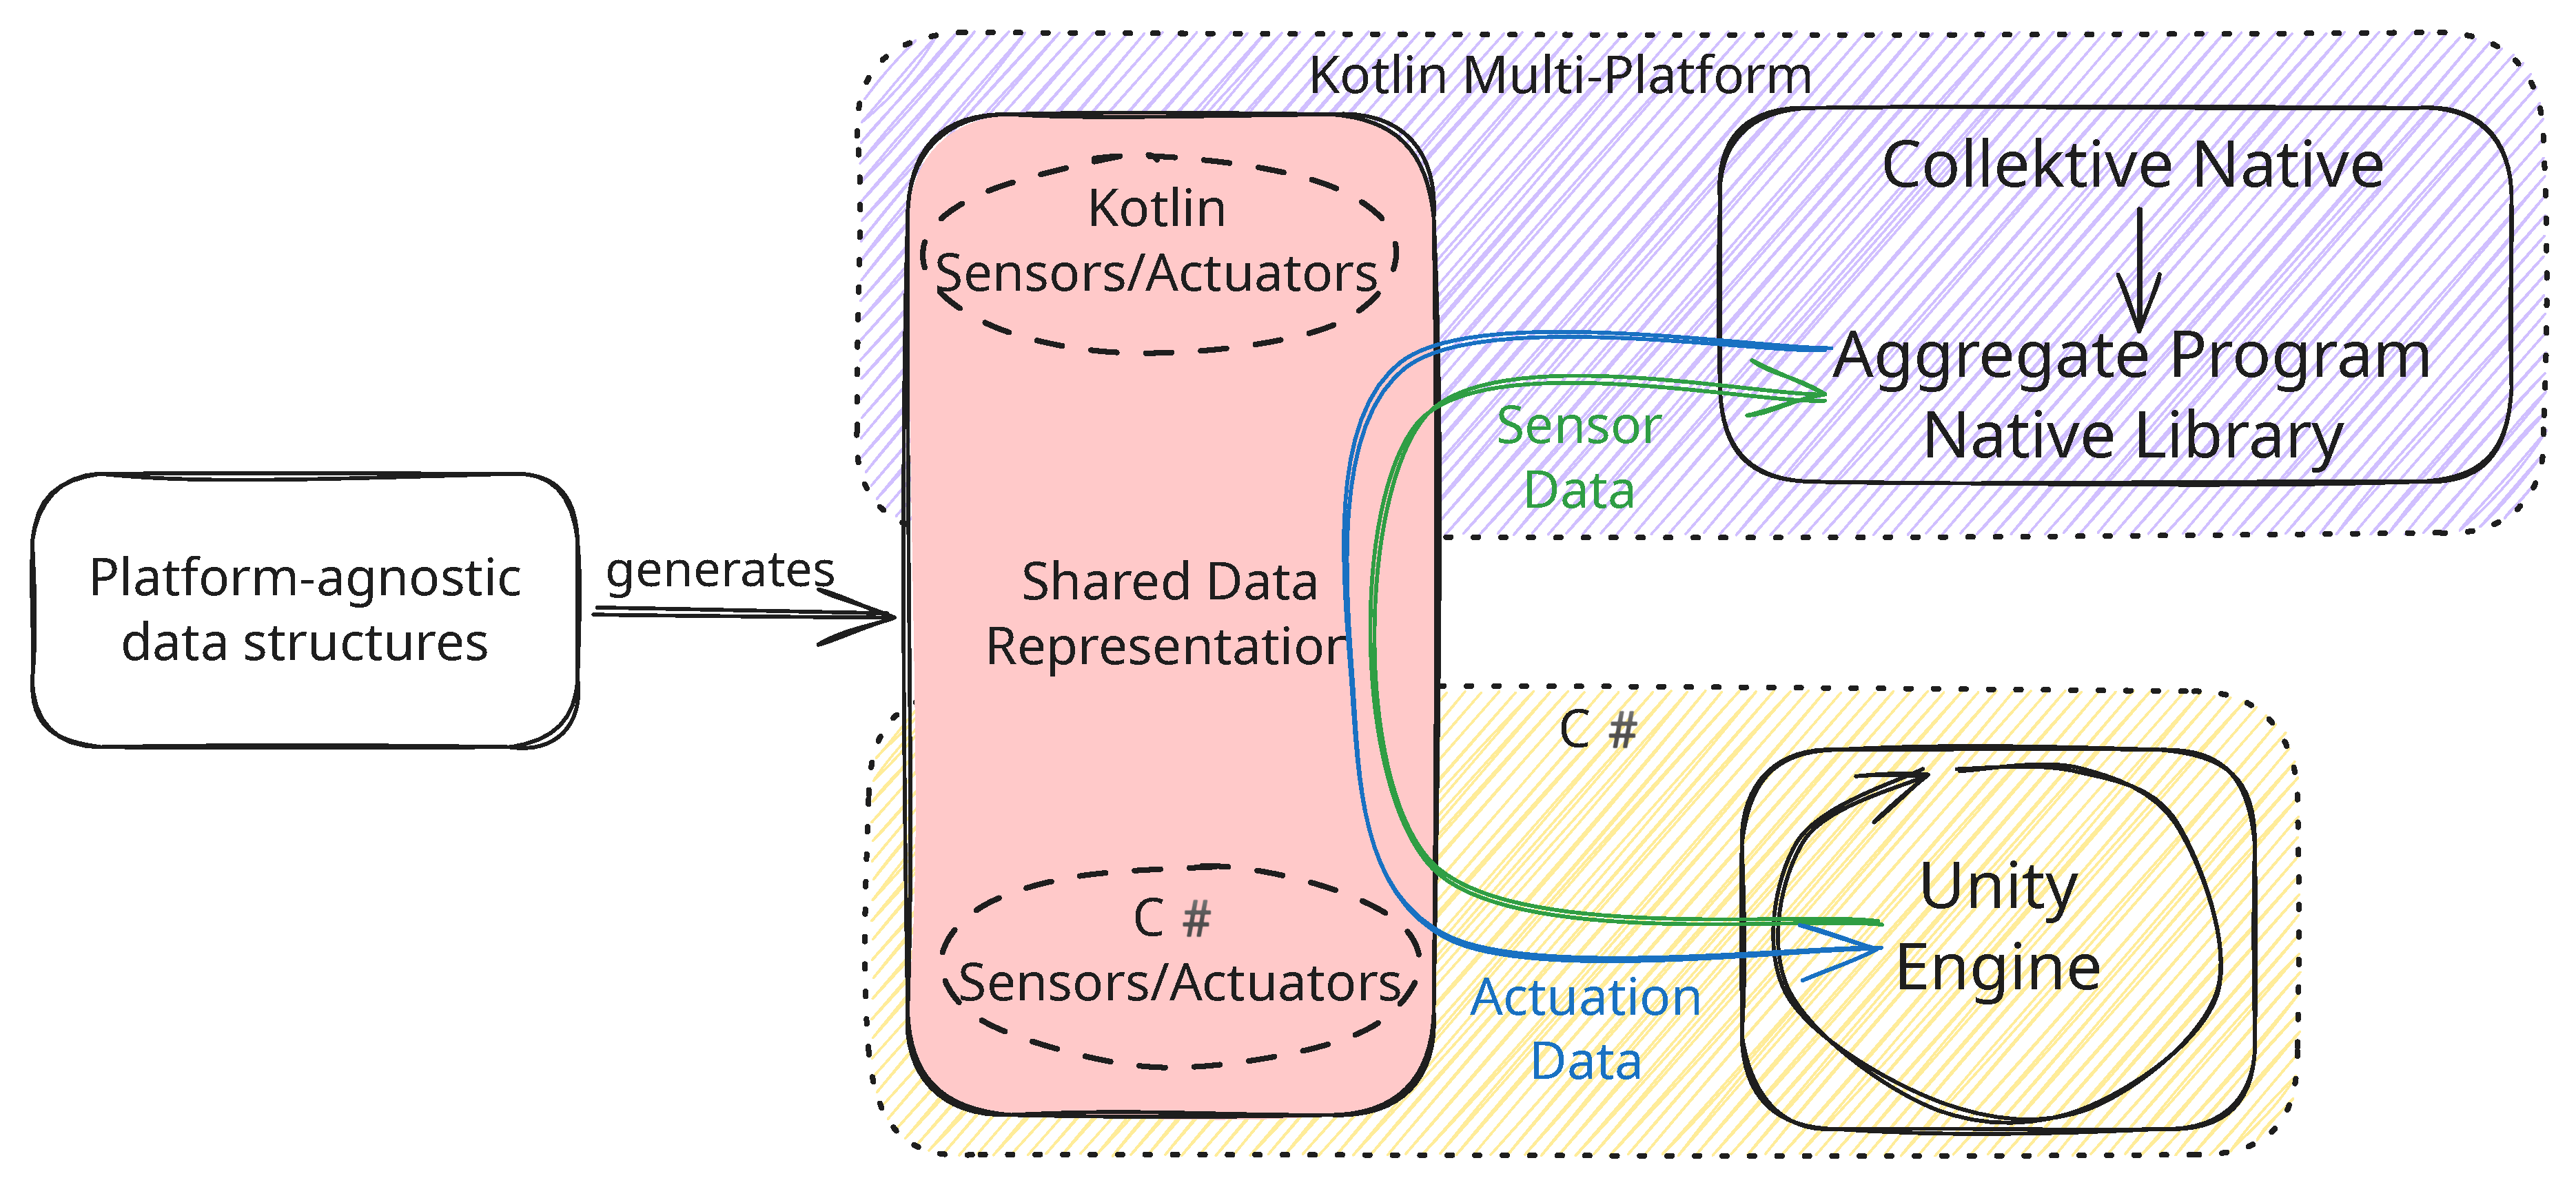
\includegraphics[width=1\textwidth]{figures/coordination26/architecture.pdf}
    \caption{High-level architecture of the integration between Collektive and Unity.
    %
    The Unity game engine provides Sensor Data to the Collektive aggregate program, 
    which computes Actuation Data that is sent back to the engine.
    %
    The Shared Data Representation layer allows users to define Sensors and Actuators data schema using platform-agnostic data structures,
    which are then used to automatically generate concrete data types for both platforms (i.e., Kotlin for Collektive and C\# for Unity), 
    thus enabling direct communication.
    }
    \label{fig:arch}
\end{figure}

Requirements R1 and R2 induce an architecture where data that flows between the two platforms
is structured according to a shared schema, which must be flexible enough to accommodate different use cases.
%
Since the device behavior is defined by the aggregate program,
while the environment behavior
(including physics, position in the world, and neighborhood relationships)
pertain to the game engine,
the natural division of responsibilities is to have the game engine provide sensory data to the aggregate program,
while the aggregate program computes the actuation commands back to the engine.

This architectural choice implication is that, when designing new case studies,
users must, as first step,
define the data types that represent sensors and actuators.
%
These must constitute an \emph{agnostic} layer,
expressed in a platform-agnostic format,
that must, in turn, generate bindings that enable communication between the two platforms.

Architecturally,
Unity is designed as an active component hosting a game loop,
while Collektive is designed to be executable in a purely functional style
(indeed, every aggregate program is a pure function from previous state, sensor inputs,
and neighbour messages to new state, actuation commands, and outgoing messages):
this clearly suggests that Unity should drive the execution,
and Collektive should be invoked as a library to compute the next state and actuation commands at each step of the game loop.

The architecture resulting from these considerations is illustrated in \cref{fig:arch}:
the agnostic layer generates bindings for C\# and Kotlin,
plus a shared schema for the data that flows between the two platforms.
%
Unity is the active component,
which, at each step of the game loop,
\begin{inlinelist}
    \item collects sensory data from the environment
    \item calls Collektive providing the data as input, and
    \item applies the actuation commands based on the data returned by Collektive.
\end{inlinelist}

\subsection{Integration design}\label{subsec:integration-design}

\begin{figure}
    \centering
    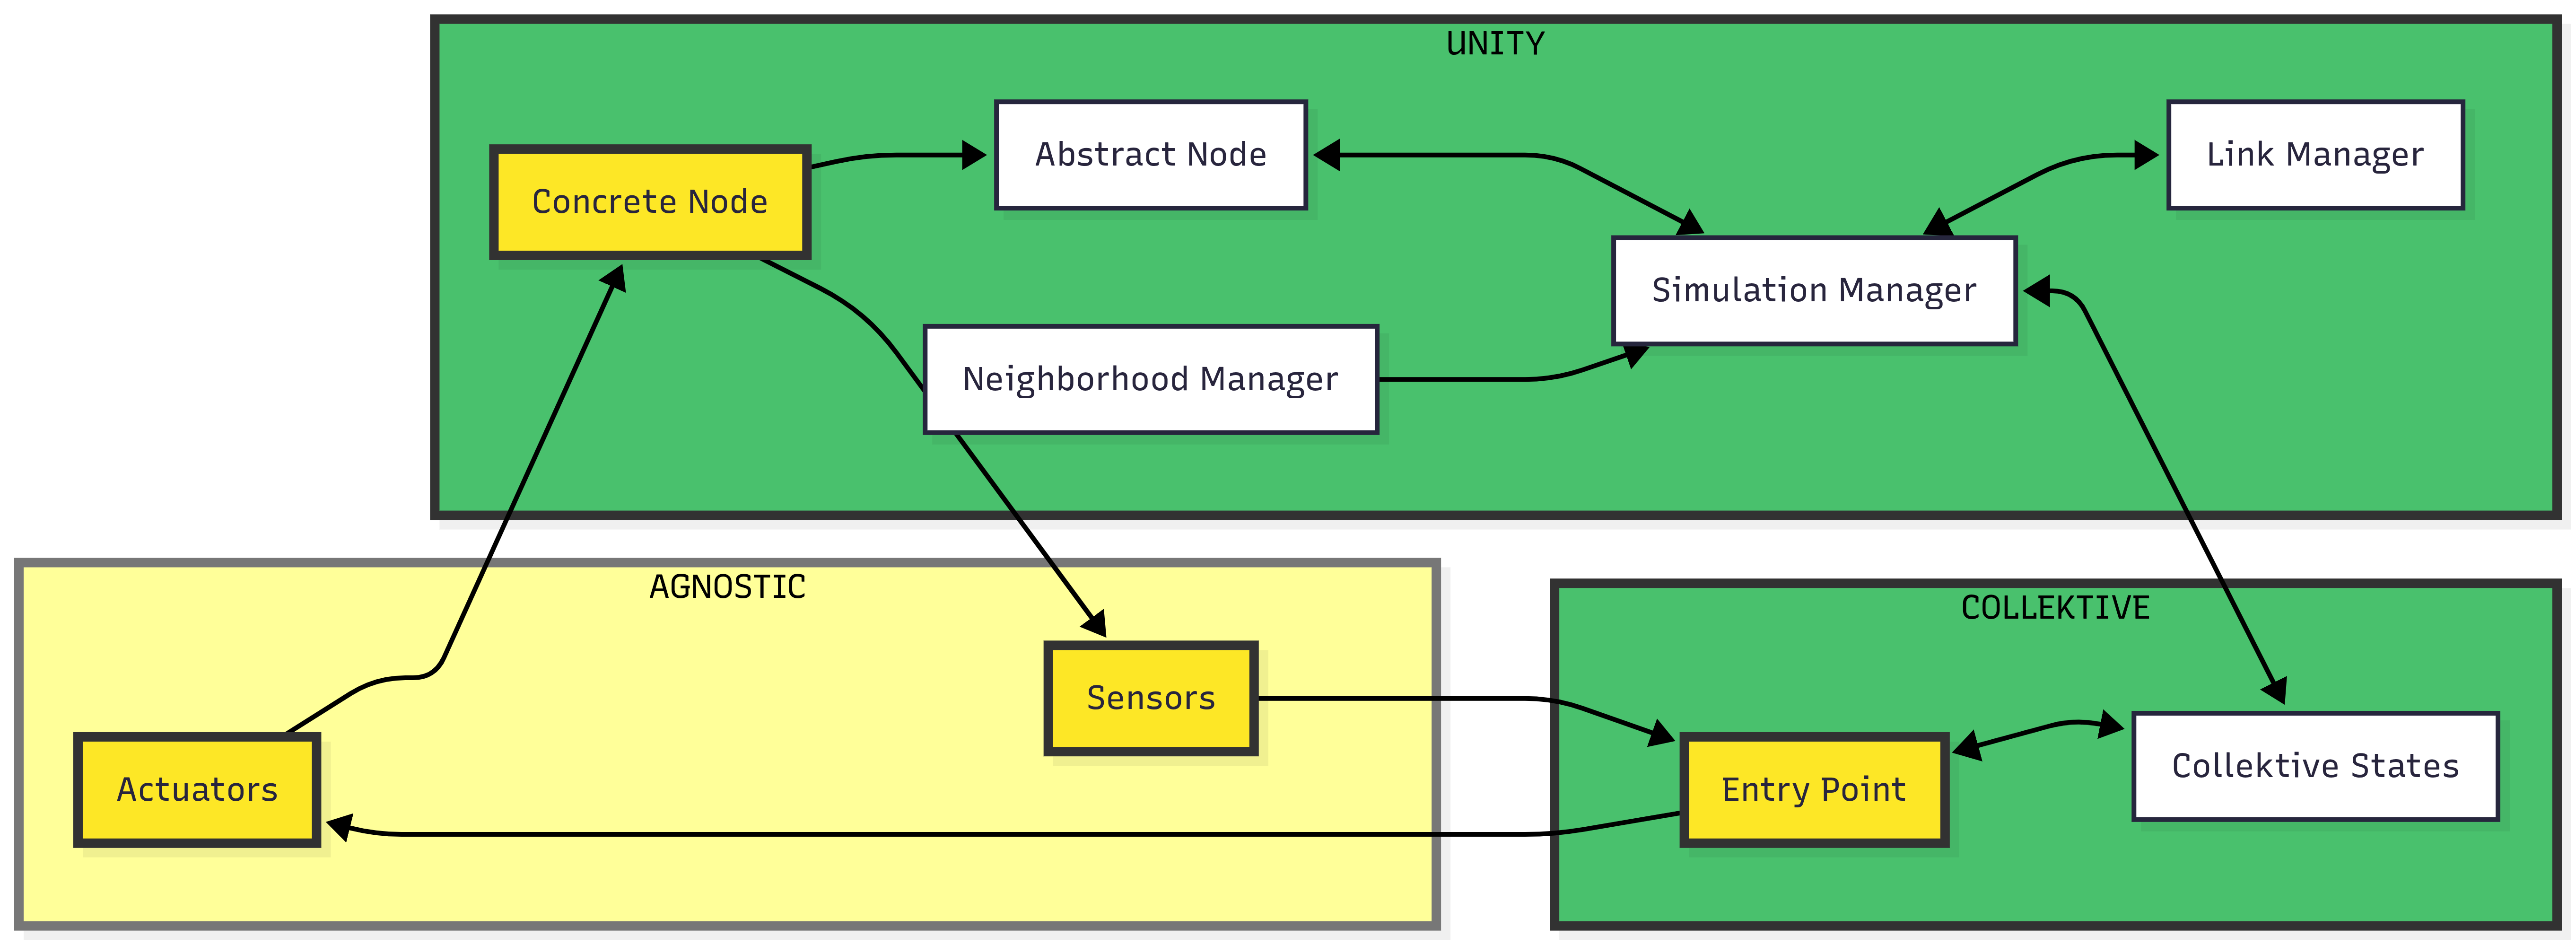
\includegraphics[width=1\textwidth]{figures/coordination26/design}
    \caption{
        Design of the integration layer between Collektive and Unity.
        Components highlighted in yellow must be implemented by the final user.
    }\label{fig:design}
\end{figure}

This section details the design of the integration layer that couples Unity's execution model with the Collektive runtime.
The design follows the architectural decomposition in \cref{fig:design}, separating
\begin{inlinelist}
    \item the \emph{environment layer} (Unity),
    \item the \emph{aggregate layer} (Collektive),
    and
    \item an \emph{agnostic data layer} that defines what information flows between the two.
\end{inlinelist}

\subsubsection{Agnostic data layer: sensors and actuators.}\label{sec:agnostic-data-layer}
Requirements R1 and R2 imply that the integration cannot hard-code any specific notion of sensing or actuation.
%
Instead, Collektivity exposes a thin, platform-independent contract expressed as two families of data types:
\emph{Sensors} (from Unity to Collektive) and \emph{Actuators} (from Collektive to Unity).
%
From this contract, the toolchain generates strongly typed bindings for both C\# and Kotlin, plus the marshaling code needed
to exchange values across runtimes.
%
Practically, this is realized via an \ac{IDL}-driven workflow: users describe the schema once, and code generation produces
compatible representations on both sides.
%
This choice keeps the interface stable while allowing each case study to tailor the exchanged data to its needs.

The agnostic data layer must, in the general case, be provided by the user,
as it is scenario-specific; however,
since most scenarios will likely share common sensing and actuation patterns (e.g., position, velocity, proximity, light intensity, etc.),
in the future a library of common schemas and bindings could be provided to reduce the initial overhead for new users.

%\paragraph{Native bridge and \ac{FFI}.}
%Unity scripts execute on a .NET runtime, while Collektive programs target Kotlin and, in our project, are compiled to native code.
%%
%Communication between the two can be achieved through various inter-process communication mechanisms
%(e.g., sockets, shared files, or higher-level protocols),
%or, to avoid the overhead and complexity of inter-process communication, \ac{FFI}.
%%
%Later in the paper, we'll show two implementations, based on socket and \ac{FFI}, and discuss their trade-offs.

\subsubsection{Unity-side runtime.}
Collektivity follows Unity's composition model, where behavior is defined by attaching \texttt{MonoBehaviour} components to \emph{game objects}.
The integration provides three core components.
%
\texttt{SimulationManager}
centralizes reproducibility concerns (e.g., deterministic initialization via explicit seeds) and exposes an API to create and manage links.
%
\texttt{AbstractNode} marks a game object as a Collektive device.
It defines the extension points that are scenario-specific:
how sensor data is sampled from the Unity world, and how actuator commands are applied.
%
Concrete scenarios are implemented by subclassing \texttt{AbstractNode} (e.g., \texttt{ConcreteNode} in \cref{fig:design}) and providing the
domain logic for sensing and actuation, while reusing the integration-provided communication and execution machinery.
%
\texttt{LinkManager} is a visualization-oriented singleton that maintains and renders the current network links (when enabled),
decoupling debugging/inspection concerns from simulation logic.

Aggregate programs depend on neighbor exchange, 
but the definition of \emph{who is a neighbor} is inherently situated and environment-dependent.
%
In Collektivity, 
neighborhood construction is handled by Unity, which creates and removes directed or bidirectional links through the
\texttt{SimulationManager} \ac{API}.
%
This enables multiple strategies, ranging from geometric proximity to occlusion-aware connectivity.
%
An efficient pattern leverages Unity's physics system and trigger colliders;
for instance, a connection rule component that automatically subscribes/unsubscribes links when other nodes enter/exit a proximity
volume can be implemented by annotating the implementing class with an attribute,
whose \texttt{OnTriggerEnter} and \texttt{OnTriggerExit} methods call the appropriate link-management \ac{API} to maintain the neighborhood structure.
%
%\begin{verbatim}
%[RequireComponent(typeof(Collider))]
%public class ProximityNeighborhoodBehaviour : MonoBehaviour {
%  private Collider _collider;
%  private Node _node;
%
%  private void Start() {
%    _collider = GetComponent<Collider>();
%    _node = GetComponentInParent<Node>();
%  }
%
%  private void OnTriggerEnter(Collider other) {
%    var otherNode = other.GetComponent<Node>();
%    if (otherNode != null) {
%      SimulationManager.Instance.Subscribe(_node, otherNode);
%    }
%  }
%
%  private void OnTriggerExit(Collider other) {
%    var otherNode = other.GetComponent<Node>();
%    if (otherNode != null) {
%      SimulationManager.Instance.Unsubscribe(_node, otherNode);
%    }
%  }
%}
%\end{verbatim}
%
By delegating neighborhood dynamics to Unity, the integration can directly reuse engine-level facilities (collisions, triggers, layers, and spatial
partitioning), while keeping the Collektive runtime agnostic of the specific spatial model.

At each simulation tick, Unity performs the following steps for each node:
\begin{inlinelist}
    \item sample sensors from the world state,
    \item invokes the Collektive adapter,
    which evaluates the aggregate program provided the most recent messages from current neighbors and the last device state,
    returning actuation commands,
    and
    \item apply actuators to Unity objects.
\end{inlinelist}
%
This design preserves the functional structure of aggregate rounds while fitting Unity's imperative update loop, and provides a single place
(\texttt{SimulationManager}) to enforce scheduling policies (e.g., fixed-rate stepping) and to coordinate message delivery.

Collektivity provides the implementation for the \texttt{SimulationManager}, the \texttt{AbstractNode}, and the \texttt{LinkManager},
plus the code-generation workflow for Sensors/Actuators.
%
Scenario developers provide:
\begin{inlinelist}
    \item the sensor/actuator schema,
    \item concrete node components that interpret the schema and implement sensing/actuation, and
    \item neighborhood rules implemented as Unity components that call the link-management \ac{API}.
\end{inlinelist}

\subsubsection{Collective-side \ac{API}}\label{subsec:collective-api}

On the Collektive side, Collektivity exposes a minimal \ac{API} that wraps the execution engine and
presents it as a stateful service to the Unity runtime.
This \ac{API} has two goals:
\begin{inlinelist}
    \item provide Unity with a stable entry point to advance the aggregate computation for each device, and
    \item internalize all program-dependent artifacts (in particular, neighbor message contents and device state),
    so that the Unity integration remains independent of the specific aggregate program.
\end{inlinelist}

In aggregate computing, the shape of the messages exchanged among neighbors is not an application-level design choice:
it is induced by the program structure and by the compilation strategy of the underlying calculus~\cite{DBLP:journals/tocl/AudritoVDPB19}.
%
Consequently, modeling messages as part of the Unity-side schema would undermine R1:
every change in the aggregate program could require regenerating schemas and bindings and revising Unity-side code,
which is not sustainable for iterative development and experimentation.
%
For this reason, Collektivity treats neighbor messaging as an internal concern of the Collektive runtime, not as part of the
Sensors/Actuators contract.
%
Thus, the collective-side \ac{API} maintains, for each simulated device:
\begin{inlinelist}
    \item the latest \emph{device state} produced by the aggregate program (used to support stateful constructs across rounds),
    \item the most recent \emph{inbound messages} received from current neighbors, and
    \item the \emph{outbound messages} generated in the last round, which will be delivered to neighbors according to the topology provided by Unity.
\end{inlinelist}
In addition, it stores the association between Unity node identifiers and Collektive engine instances,
so that Unity can refer to devices through stable handles.

At each simulation tick, Unity invokes the collective-side \ac{API} to advance each device by one round.
For a given device, the \ac{API} evaluates the aggregate program against
\begin{inlinelist}
    \item the stored device state,
    \item the current sensor snapshot provided by Unity,
    and
    \item the inbound messages buffered from neighbors.
\end{inlinelist}
%
The evaluation produces a new device state, a set of outbound messages, and the actuator commands.
%
Unity then applies the returned actuators to update the game objects, and uses its current link graph to determine how outbound messages
are routed to neighbor buffers before the next tick.
%
This division of responsibilities matches the architecture in \cref{fig:design}:
Unity owns the environment and the topology,
while Collektive owns the distributed computation semantics.

\subsection{Implementation strategy}\label{subsec:implementation}

In this section,
we describe the practical construction of Collektivity,
discussing the technological choices that realize the design outlined in \Cref{subsec:integration-design}.
%
The implementation of Collektivity is publicly available\footnote{\url{https://github.com/pslab-unibo/collektivity}}
and archived for future reference~\cite{collektivity-zenodo},
and has the form of a repository template.
%
The purpose of the template is to provide a starting point for researchers and practitioners interested in
integrating experimenting with aggregate programs in Unity.

\begin{table*}[t]
    \centering
    \caption{Performance comparison between the native (\ac{FFI}) and socket-based backends.
    Times are in nanoseconds (ns), lower is better.
    Speedup is reported as Socket/Native (higher is worse for sockets).}
    \label{tab:backend-frontend-benchmark}
    \setlength{\tabcolsep}{6pt}
    \renewcommand{\arraystretch}{1.15}
    \begin{tabular}{l | r | r | r | r | r | r}
        \hline
        \textbf{Metric} & \multicolumn{3}{c |}{\textbf{Overhead Collektive-side}} & \multicolumn{3}{c}{\textbf{End-to-end (ns)}} \\
        \cline{2-4}\cline{5-7}
        & \textbf{FFI} & \textbf{Socket} & \textbf{Speedup} & \textbf{Native} & \textbf{Socket} & \textbf{Speedup} \\
        \hline
        count  & 970 & 969 & -- & 969 & 968 & -- \\
        median & 13830 & 137857 & 11.20$\times$ & 550600 & 200001950 & 363.32$\times$ \\
        mean   & 13175 & 170269 & 13.86$\times$ & 484754 & 199963813 & 456.26$\times$ \\
        p95    & 16597 & 348890 & 28.02$\times$ & 612140 & 200560775 & 719.35$\times$ \\
        p99    & 36306 & 456583 & 41.25$\times$ & 850520 & 202753798 & 747.95$\times$ \\
        std    & 4843  & 265368 & -- & 141814 & 3265095 & -- \\
        \hline
    \end{tabular}
\end{table*}

As first step to head into implementation,
we built an experimental prototype with 12 nodes to compare the performance of two communication strategies
through a simple benchmark that simulates the core communication pattern of Collektive programs:
\begin{inlinelist}
    \item a socket-based backend, where Unity and Collektive run as separate processes and exchange data through TCP sockets, and
    \item a native backend, where Collektive is compiled to a shared library and directly invoked by Unity through \ac{FFI}.
\end{inlinelist}
%
We expected better performance for the latter,
but the former has the advantage of being more flexible,
as any Collektive target could be used,
instead of limiting the support to the native compilation targets.
%
The benchmark is publicly available\footnote{
    \scriptsize
    \url{https://github.com/pslab-unibo/experiment-2026-coordination-collektive-unity-benchmark}
} and archived for future reference~\cite{benchmark-zenodo}.
%
\Cref{tab:backend-frontend-benchmark} summarizes the results.
%
The performance difference is stark: the socket-based backend is, on average,
over 450x slower than the native backend,
with a worst-case slowdown of over 700x.
%
Provided the relevance of R3, we adopted the native compilation strategy for the integration,
and we designed the agnostic data layer to support it.

\subsubsection{Data Model}\label{sec:data-model-and-serialization}

Collektive and Unity use different type systems and memory layouts.
%
As discussed in \Cref{sec:agnostic-data-layer},
a shared data model representation,
expressed in a platform-agnostic format, 
is essential to enable communication between the two platforms while maintaining flexibility and extensibility.
%
%In such way,
%users can define the data schema once,
%and the toolchain generates the bindings to its use in both platforms (i.e., C\# and Kotlin).
%
%For data representation,
%one could consider using widely adopted serialization formats---%
%for instance, JSON or XML.
%%
%In order make use of such information representation,
%both Collektive and Unity should additionally require to
%\begin{inlinelist}
%    \item define a common schema for the data to be exchanged, which is dependent on the specific requirements of the application, and
%    \item provide parsers and serializers implementations for each information schema.
%\end{inlinelist}
%%
%Such approach, howerver,
%lacks efficiency, because the modification of the data schema must be reflected on both C\# and Kotlin code,
%therefore not satisfying requirement R1.
%%
%Moreover,
%type-safety is not guaranteed,
%as the data is represented as unstructured text.
%
%There exist other approaches to data representation and serialization that can better fit
%the requirements of our integration.
%
\emph{Protocol Buffers}\footnote{\url{https://protobuf.dev/}} (\texttt{protobuf}) is a language-neutral,
platform-neutral mechanism for serializing structured data.
%
Protocol Buffers defines data models using a declarative syntax (\texttt{.proto} files)
that describes their structure in an implementation-agnostic way.
%
From a single \texttt{.proto} definition,
the \texttt{protoc} compiler can generate serialization source code for multiple languages automatically,
including C\#, Kotlin, Java, and many others.
%
Protocol Buffers data structures are defined as \texttt{messages},
which are composed of fields with a type and a unique identifier (tag).
%
In our use case,
we always have exactly two messages: one for \texttt{Sensors} and one for \texttt{Actuators}
(indeed, the \texttt{message}s of protocol buffers are \emph{not} the messages that aggregate programs exchange,
rather, they describe the data that is exchanged with Unity).
%
Each field can be a primitive type (e.g., integer, string, boolean)
or a user-defined message type,
allowing for nested and complex data structures.
%
The tag is used to identify fields in the binary format, 
enabling efficient serialization and deserialization.
%
This makes Protocol Buffers fit for bridging complex data model representation for Kotlin and C\# runtimes.
%
In Collektivity, 
users define \texttt{Sensors} and \texttt{Actuators} data schema using Protocol Buffers,
the latter will then generate the necessary bindings for both platforms.
%
A minimal example of a Protocol Buffers schema for Sensors and Actuators is shown in \Cref{lst:proto-schema}.
%
Depending on the specific requirements of the application,
users can define more complex data structures.
%including nested messages, repeated fields, and optional fields.

\begin{lstlisting}[
    basicstyle=\ttfamily,
    linewidth=\textwidth,
    caption={
        Example of Protocol Buffers schema for Sensors and Actuators.
        %
        \texttt{sourceIntensity} is a \texttt{double} field used by the aggregate program to determine the direction of movement towards the destination.
        %
        \texttt{Vector3} maps a Unity 3D vector, which in this example represents the current position of the device and the target position computed by the aggregate program.
        %
        \texttt{repeated Vector3} represents a list of 3D vectors, which in this example represent obstacles positions.
        %
        The integer tags (e.g., \texttt{= 1}) are used to identify fields in the binary format.
    },
    label={lst:proto-schema},
]
message Actuators {
  Vector3 targetPosition = 1;
}
message Sensors {
  double sourceIntensity = 1;
  Vector3 currentPosition = 2;
  repeated Vector3 obstacles = 3;
}
\end{lstlisting}

%\subsection{Information Exchange between Unity and Collektive}
%
%To facilitate the flow of information between Unity and Collektive,
%a communication mechanism is required for transmitting sensor data and actuator information.
%%
%Following the requirement for high-performance interoperability (R3),
%the wo viable options for communication identified are
%\ac{FFI} and socket-based communication.
%
%\ac{FFI} allows direct interaction between different programming languages
%by enabling one language to call functions or use data types defined in another language.
%%
%In this context,
%it allows Unity (C\#) to directly invoke functions from Collektive (Kotlin).
%%
%This approach facilitates efficient data exchange without the overhead of inter-process communication.
%
%On the other hand,
%socket-based communication involves establishing a network connection between Unity and Collektive,
%allowing them to send and receive messages over a network protocol.
%%
%This approach is flexible,
%since it is based on an external and independent component (i.e. a server) which offers a standard interface between the two languages and it is stand-alone---%
%i.e., it can be developed and tested independently from the rest of the system.
%%
%To determine the most performant option that satisfies R3,
%we conducted a benchmark comparing the two methods aforementioned,
%which is detailed in \Cref{sec:case-study}.
%
%Based on the results of this benchmark,
%we chose to implement \ac{FFI} in Collektivity,
%as it provided significantly lower latency and better performance for the integration.

\subsubsection{\ac{FFI} interaction and Engine API}

Collektivity extends the Collektive runtime to support execution within the Unity environment,
to do so, it provides an \texttt{Engine} (\Cref{lst:engine-api})
that defines the contract between the aggregate program and the Unity environment---%
i.e., the operations that Unity can invoke on the Collektive runtime to execute the aggregate program and retrieve the resulting state and actuation commands.
%
\texttt{Engine} is the Collektive interface that Unity invokes to execute the aggregate computation at each simulation tick,
i.e. each update cycle in the Unity execution loop triggers the invocation 
of the \texttt{step()} function in the \texttt{Engine}.
%
This function is invoked by Unity via \ac{FFI} for each simulation node, 
which identifier is specified during invocation along with \texttt{Sensors} data structure.
%
The result returned by Collektive is an \texttt{Actuators} data structure,
which is then used by Unity to update the simulation environment accordingly.
%
\texttt{Sensors} and \texttt{Actuators} are defined in the agnostic data layer,
and their schema is defined by the user (c.f., \Cref{sec:data-model-and-serialization}).

\lstinputlisting[
    % float,
    basicstyle=\scriptsize\ttfamily,
    linewidth=\textwidth,
    language=Kotlin,
    caption={Engine API definition for Collektive library.},
    label={lst:engine-api},
]{listings/coordination26/Engine.kt}

Along with the \texttt{step()} function,
\texttt{Engine} also defines methods for
\begin{inlinelist}
    \item register a node for being neighbor of another node (i.e., using \texttt{subscribe()}), 
    \item unregister a node from being neighbor of another node (i.e., using \texttt{unsubscribe()}),
    \item add a node to the simulation (i.e., using \texttt{addNode()}), and
    \item remove a node from the simulation (i.e., using \texttt{removeNode()}).  
\end{inlinelist}
%
This infrastructure is then compiled using Collektive-native,
and it is directly invoked by Unity via \ac{FFI}.

\section{Exemplars}\label{sec:case-study}

In this section,
we show a simple and a richer exemplar that we include with Collektivity
to demonstrate its capabilities and to provide a starting point for users interested in experimenting with aggregate programming in Unity.
%
In both exemplars,
we deploy devices that must navigate towards a source of interest while avoiding obstacles,
which is a common pattern in \acp{CAS} and is relevant for a wide range of applications (e.g., search and rescue).
%
They do so through a gradient ascent strategy, with no cooperative logic is implemented for obstacle avoidance.
%
All nodes execute synchronous rounds at a fixed frequency of $20Hz$,
in which they perceive the local ``intensity'' of the source of interest (based on the distance)
and detect obstacles in their vicinity.
%
Vicinities and communication between nodes are established through a distance-based neighborhood model:
two nodes are considered neighbors if their separation is within 10 units,
which defines the connectivity graph for the aggregate computation.
%
They exchange this information with their neighbors to compute their next movement direction,
computing a vector that points to the direction of higher source intensity and away from nearby obstacles
(including other devices).
%
Gradient computations are performed through the standard library in Collektive,
which provides implementations for all the building blocks in~\cite{DBLP:journals/tomacs/ViroliABDP18}.

\subsection{Simple 3D space}

\begin{figure}
    \centering
    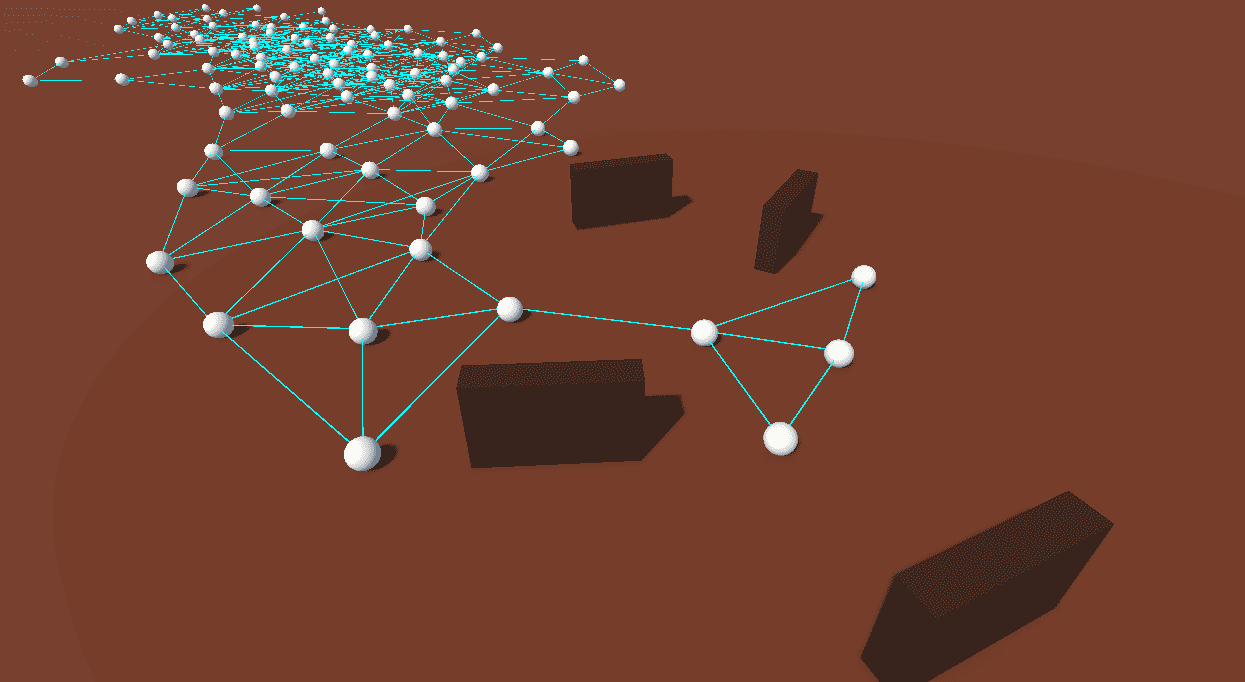
\includegraphics[width=.49\textwidth]{figures/coordination26/simple-shots/better_1}
    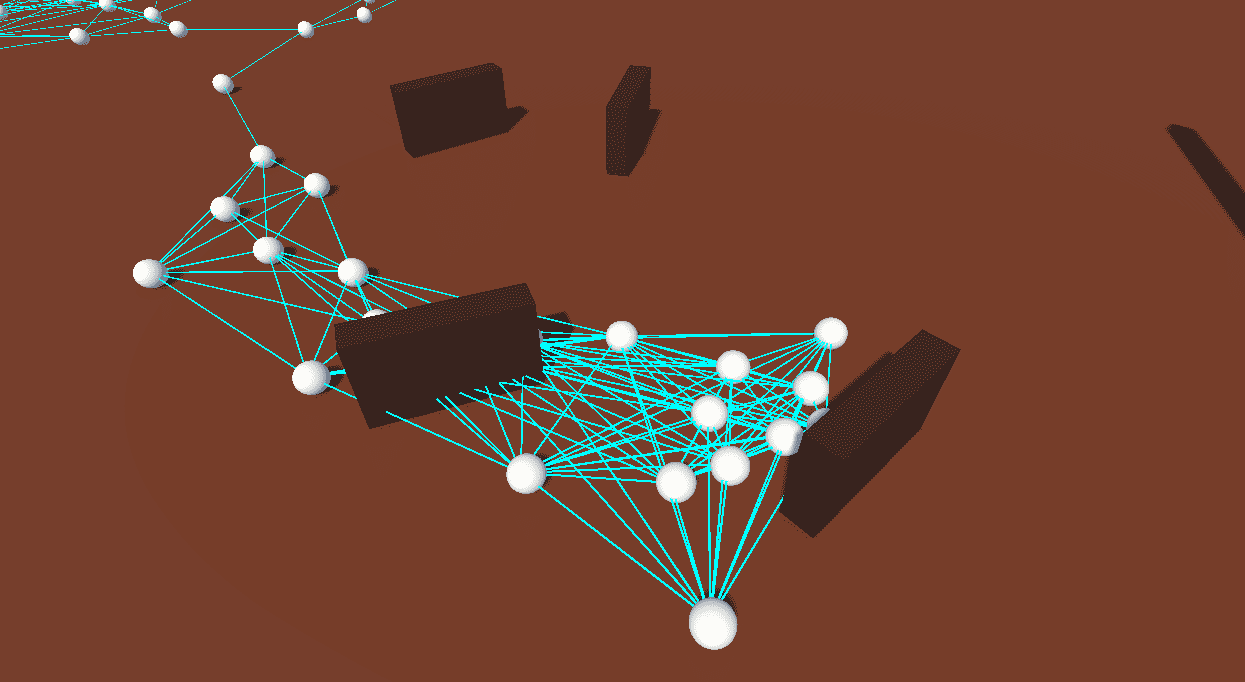
\includegraphics[width=.49\textwidth]{figures/coordination26/simple-shots/better_2}
    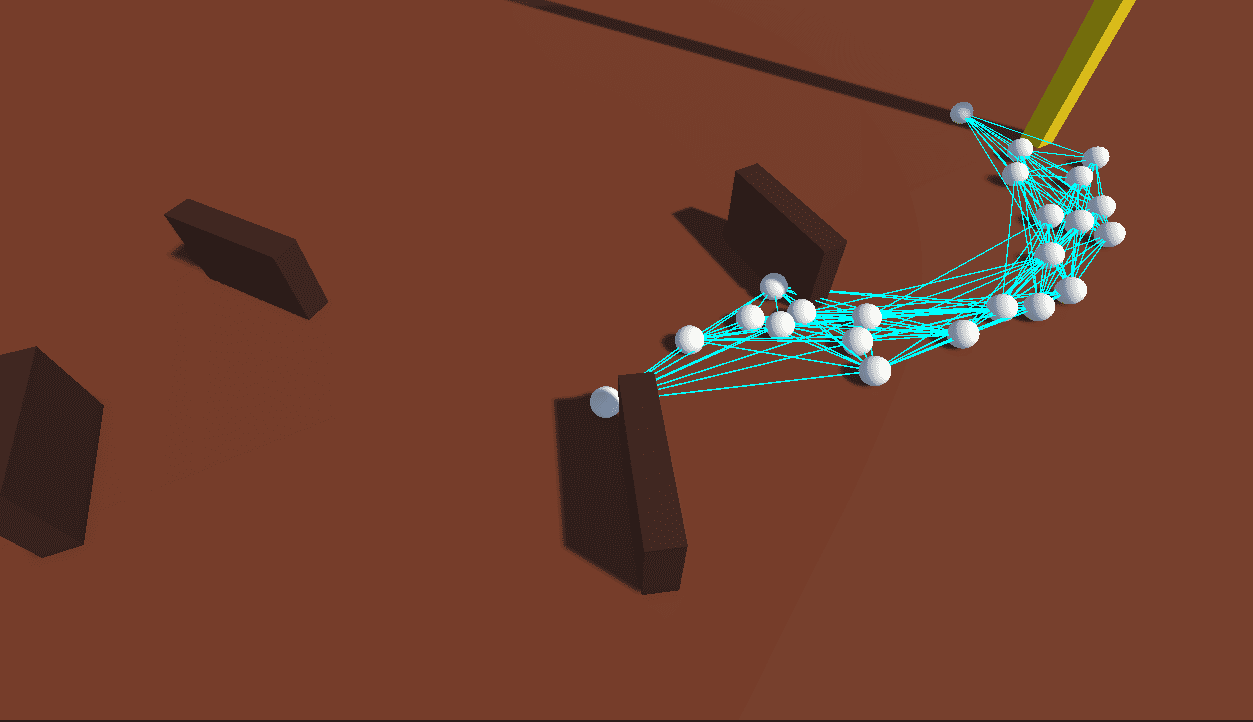
\includegraphics[width=.49\textwidth]{figures/coordination26/simple-shots/better_3}
    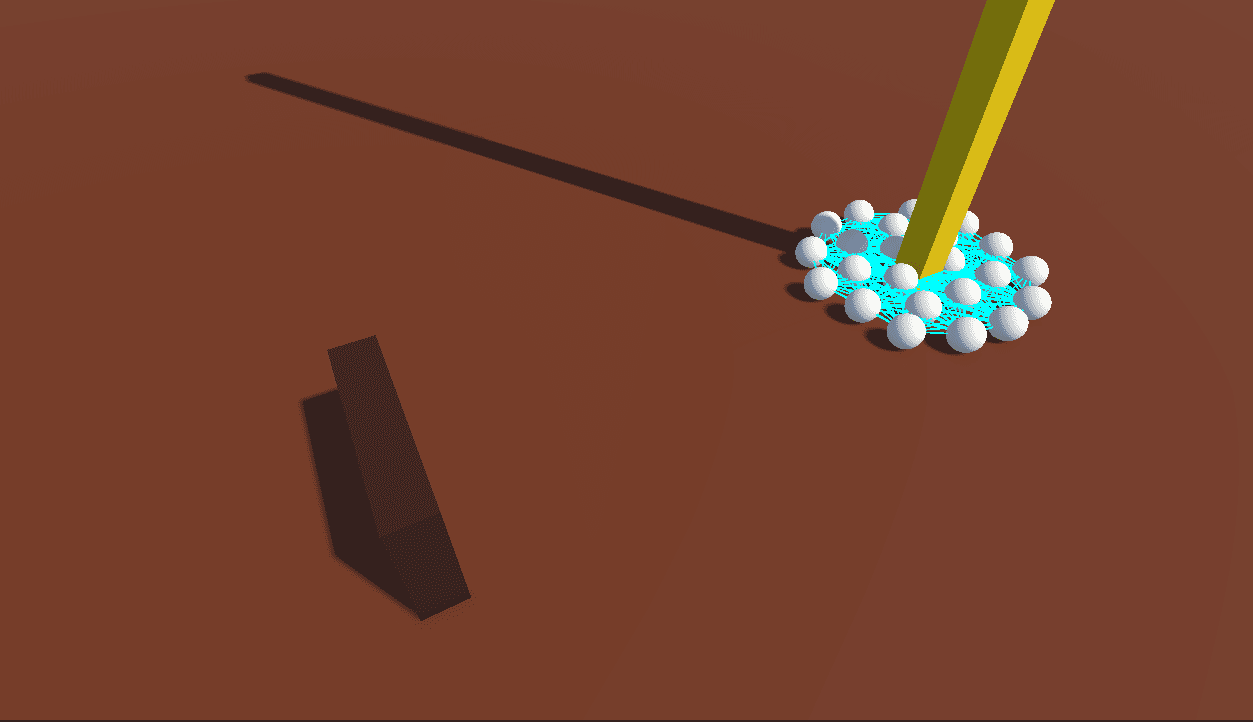
\includegraphics[width=.49\textwidth]{figures/coordination26/simple-shots/better_4}
    \caption{Snapshots of the simple 3D space scenario with 100 nodes.}\label{fig:simple}
\end{figure}

Here, we consider a simple arena with
four parallelepipedic obstacles that physically obstruct the movement towards the source.
The environment contains  of $1 \times 3 \times 5$ units.
%
Devices are represented by spheres that can move in the 3D space,
and the arena is a flat plane with a source of interest located at a fixed position.
%
We tested the scenario with different numbers of nodes.
%
Laptops with integrated graphics could achieve reasonable real-time performance with up to 50 nodes,
while we easily scaled to 100 nodes on a desktop with a dedicated GPU (nVidia GTX 4070).
%
Snapshots in \Cref{fig:simple} show the evolution of the system with 100 nodes.

\subsection{Richer environment}

%\danilo{fate una selezione di quattro snapshot fra quelli che ho messo in images/complex e fate un'immagine migliore}

\begin{figure}
    \centering
    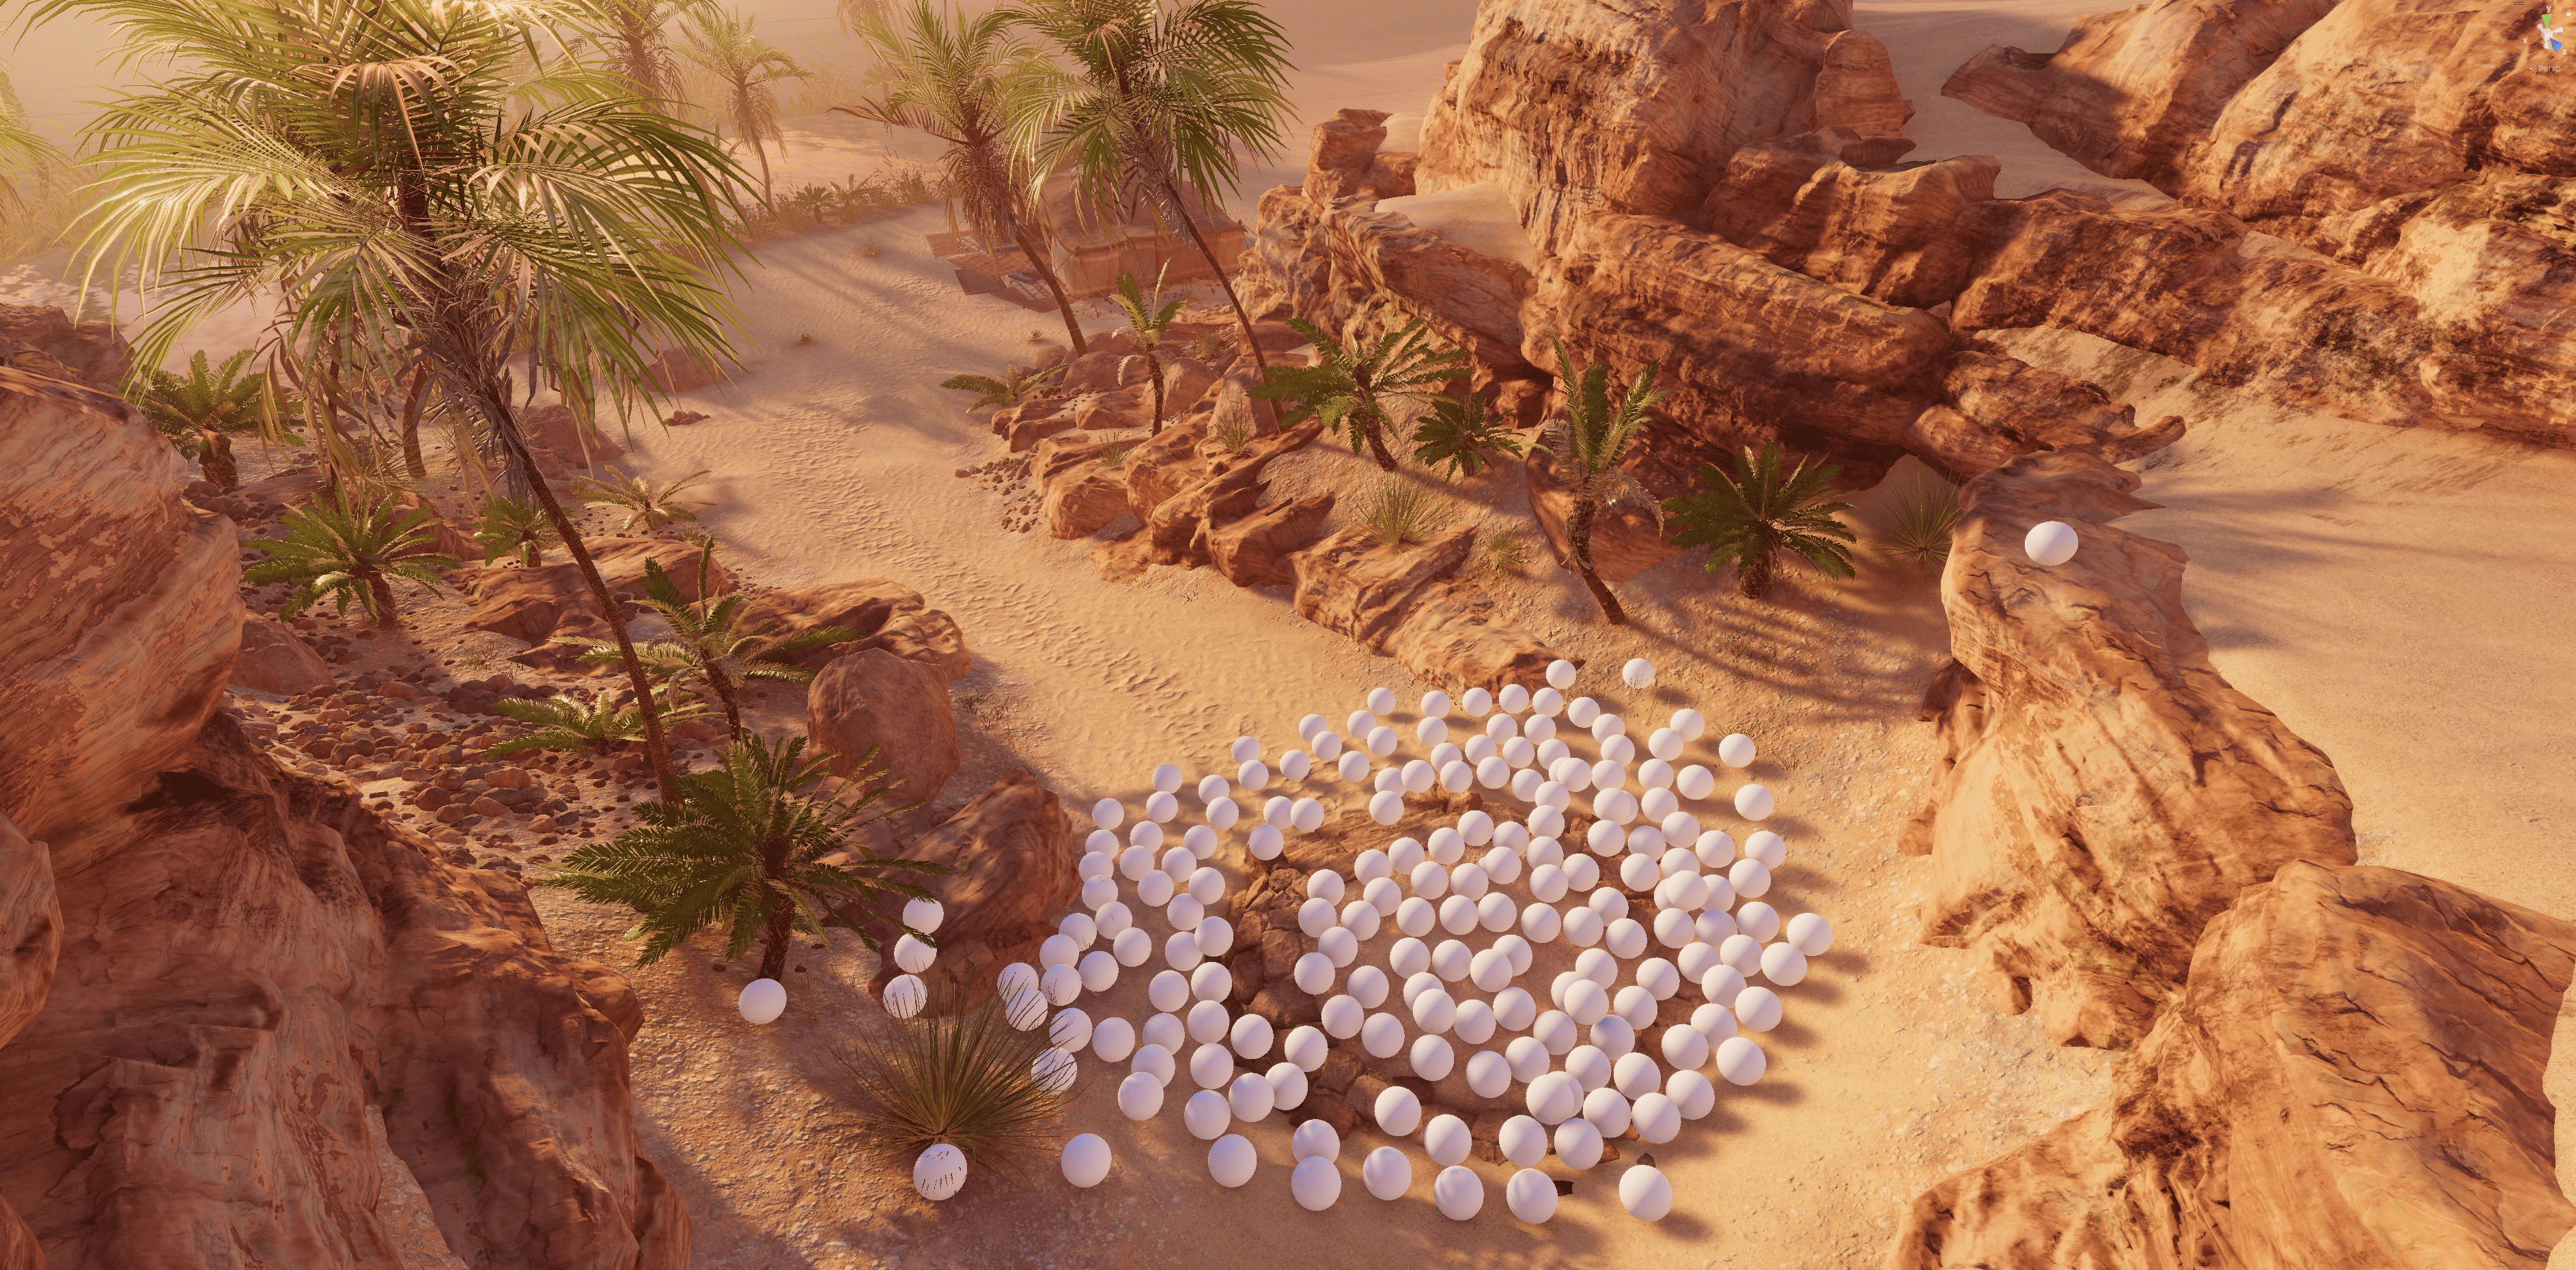
\includegraphics[width=.49\textwidth]{figures/coordination26/oasis/02}
    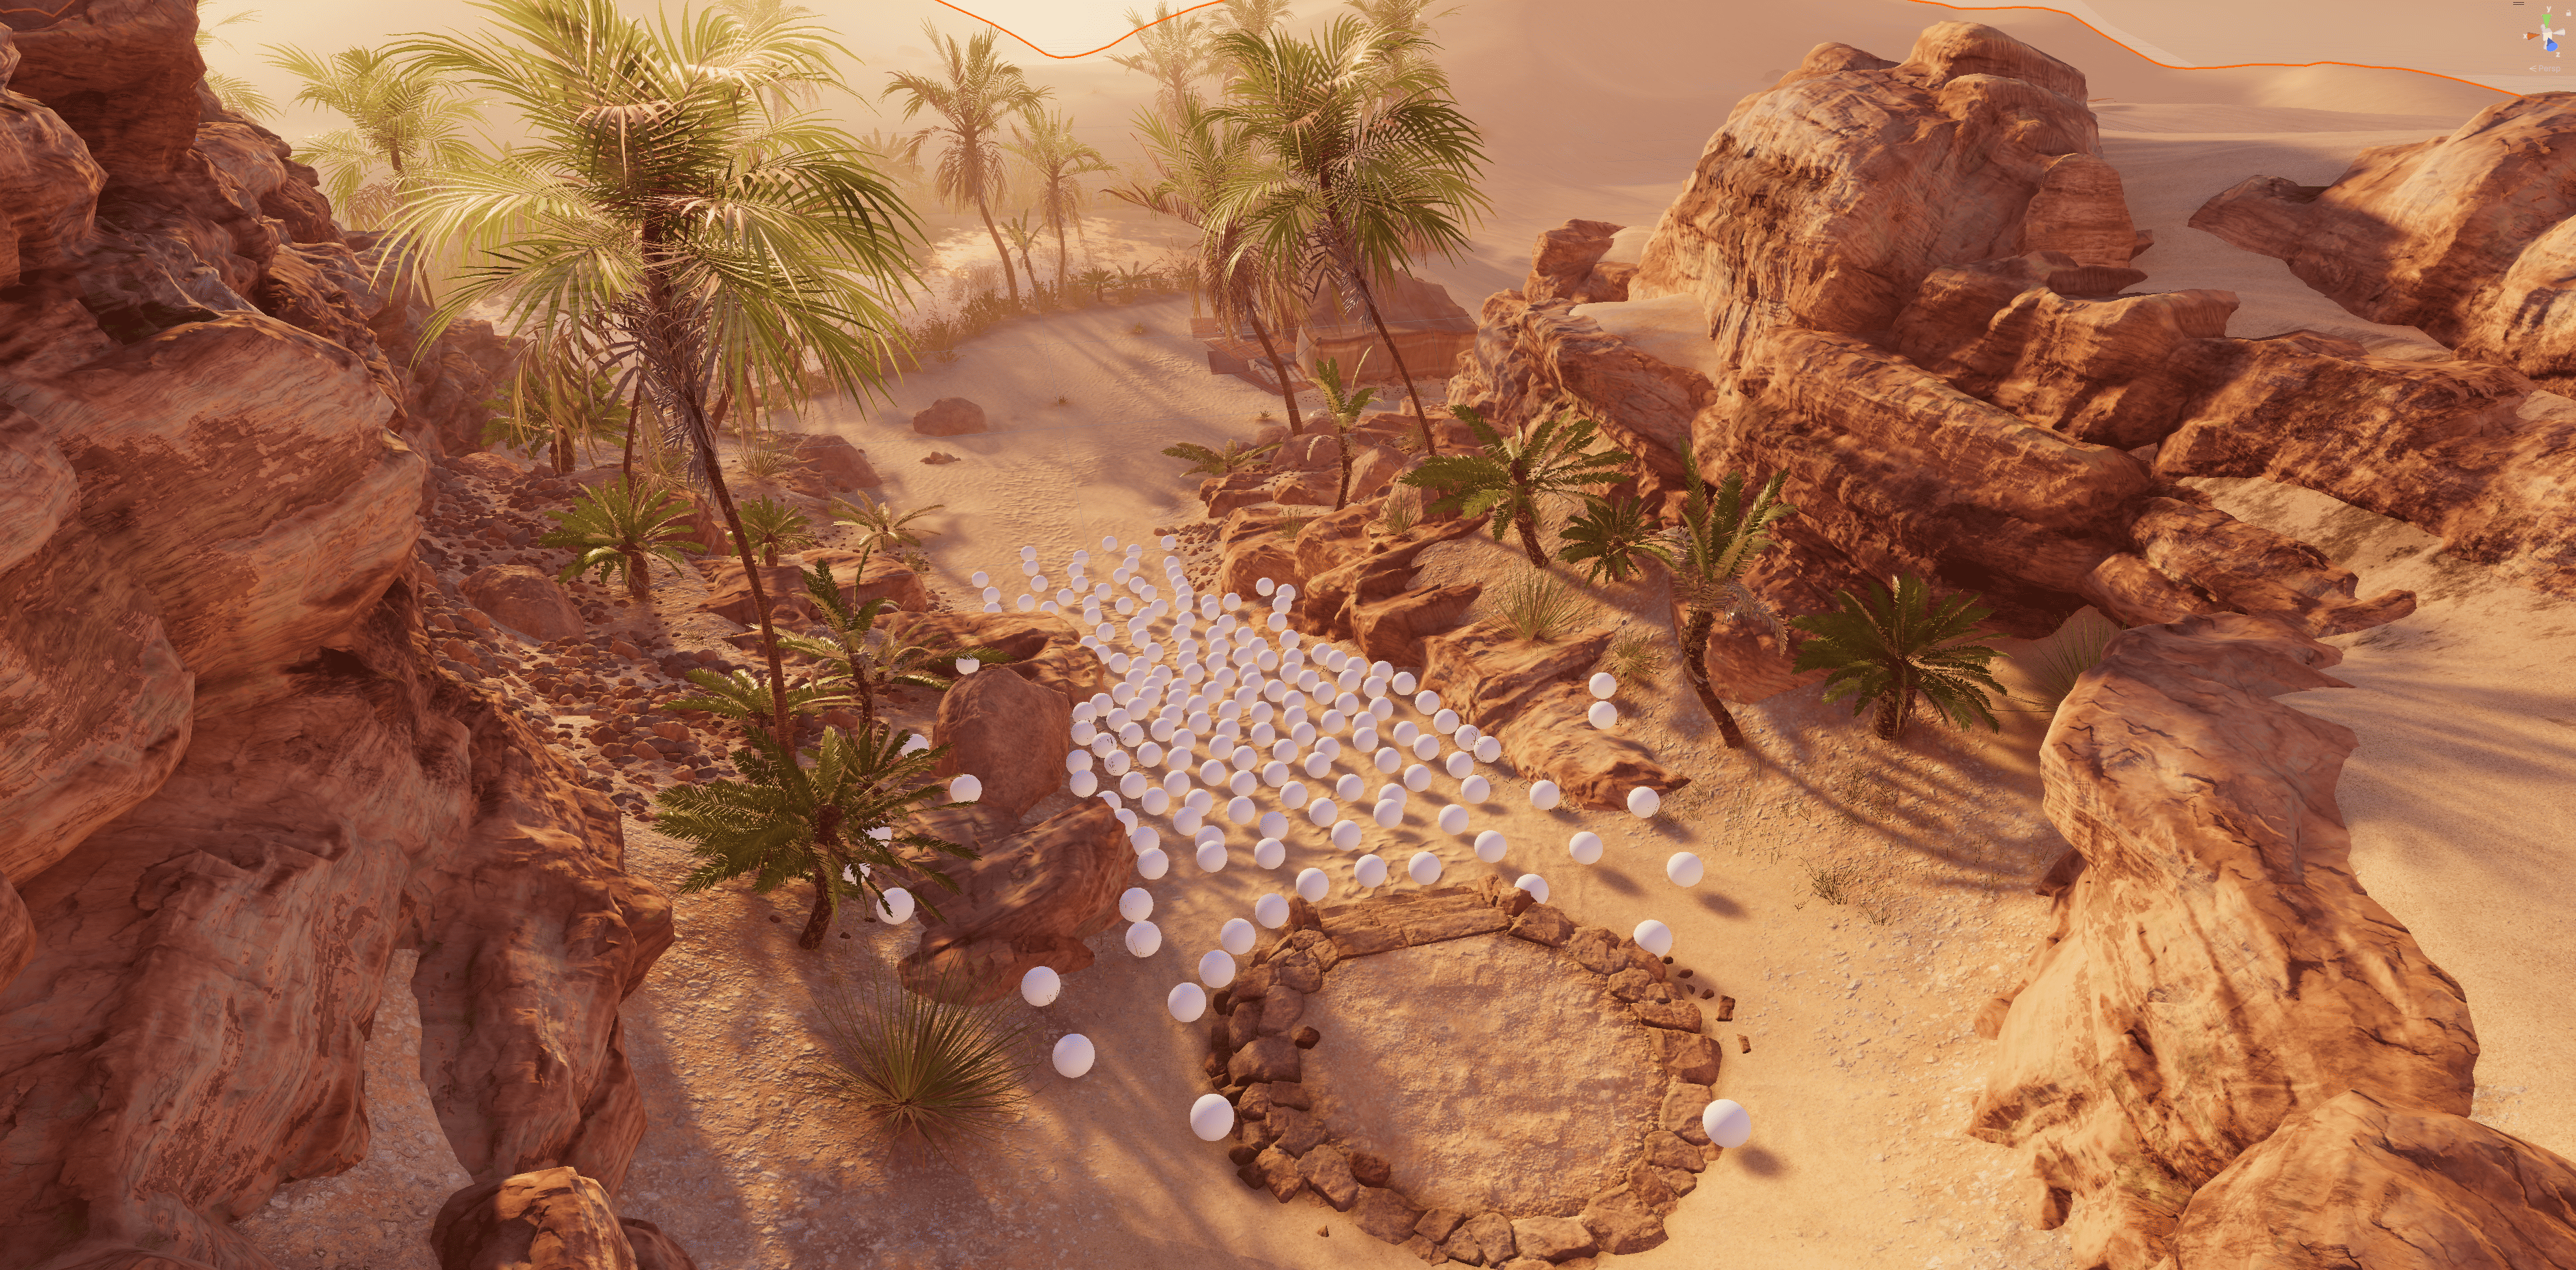
\includegraphics[width=.49\textwidth]{figures/coordination26/oasis/03}
    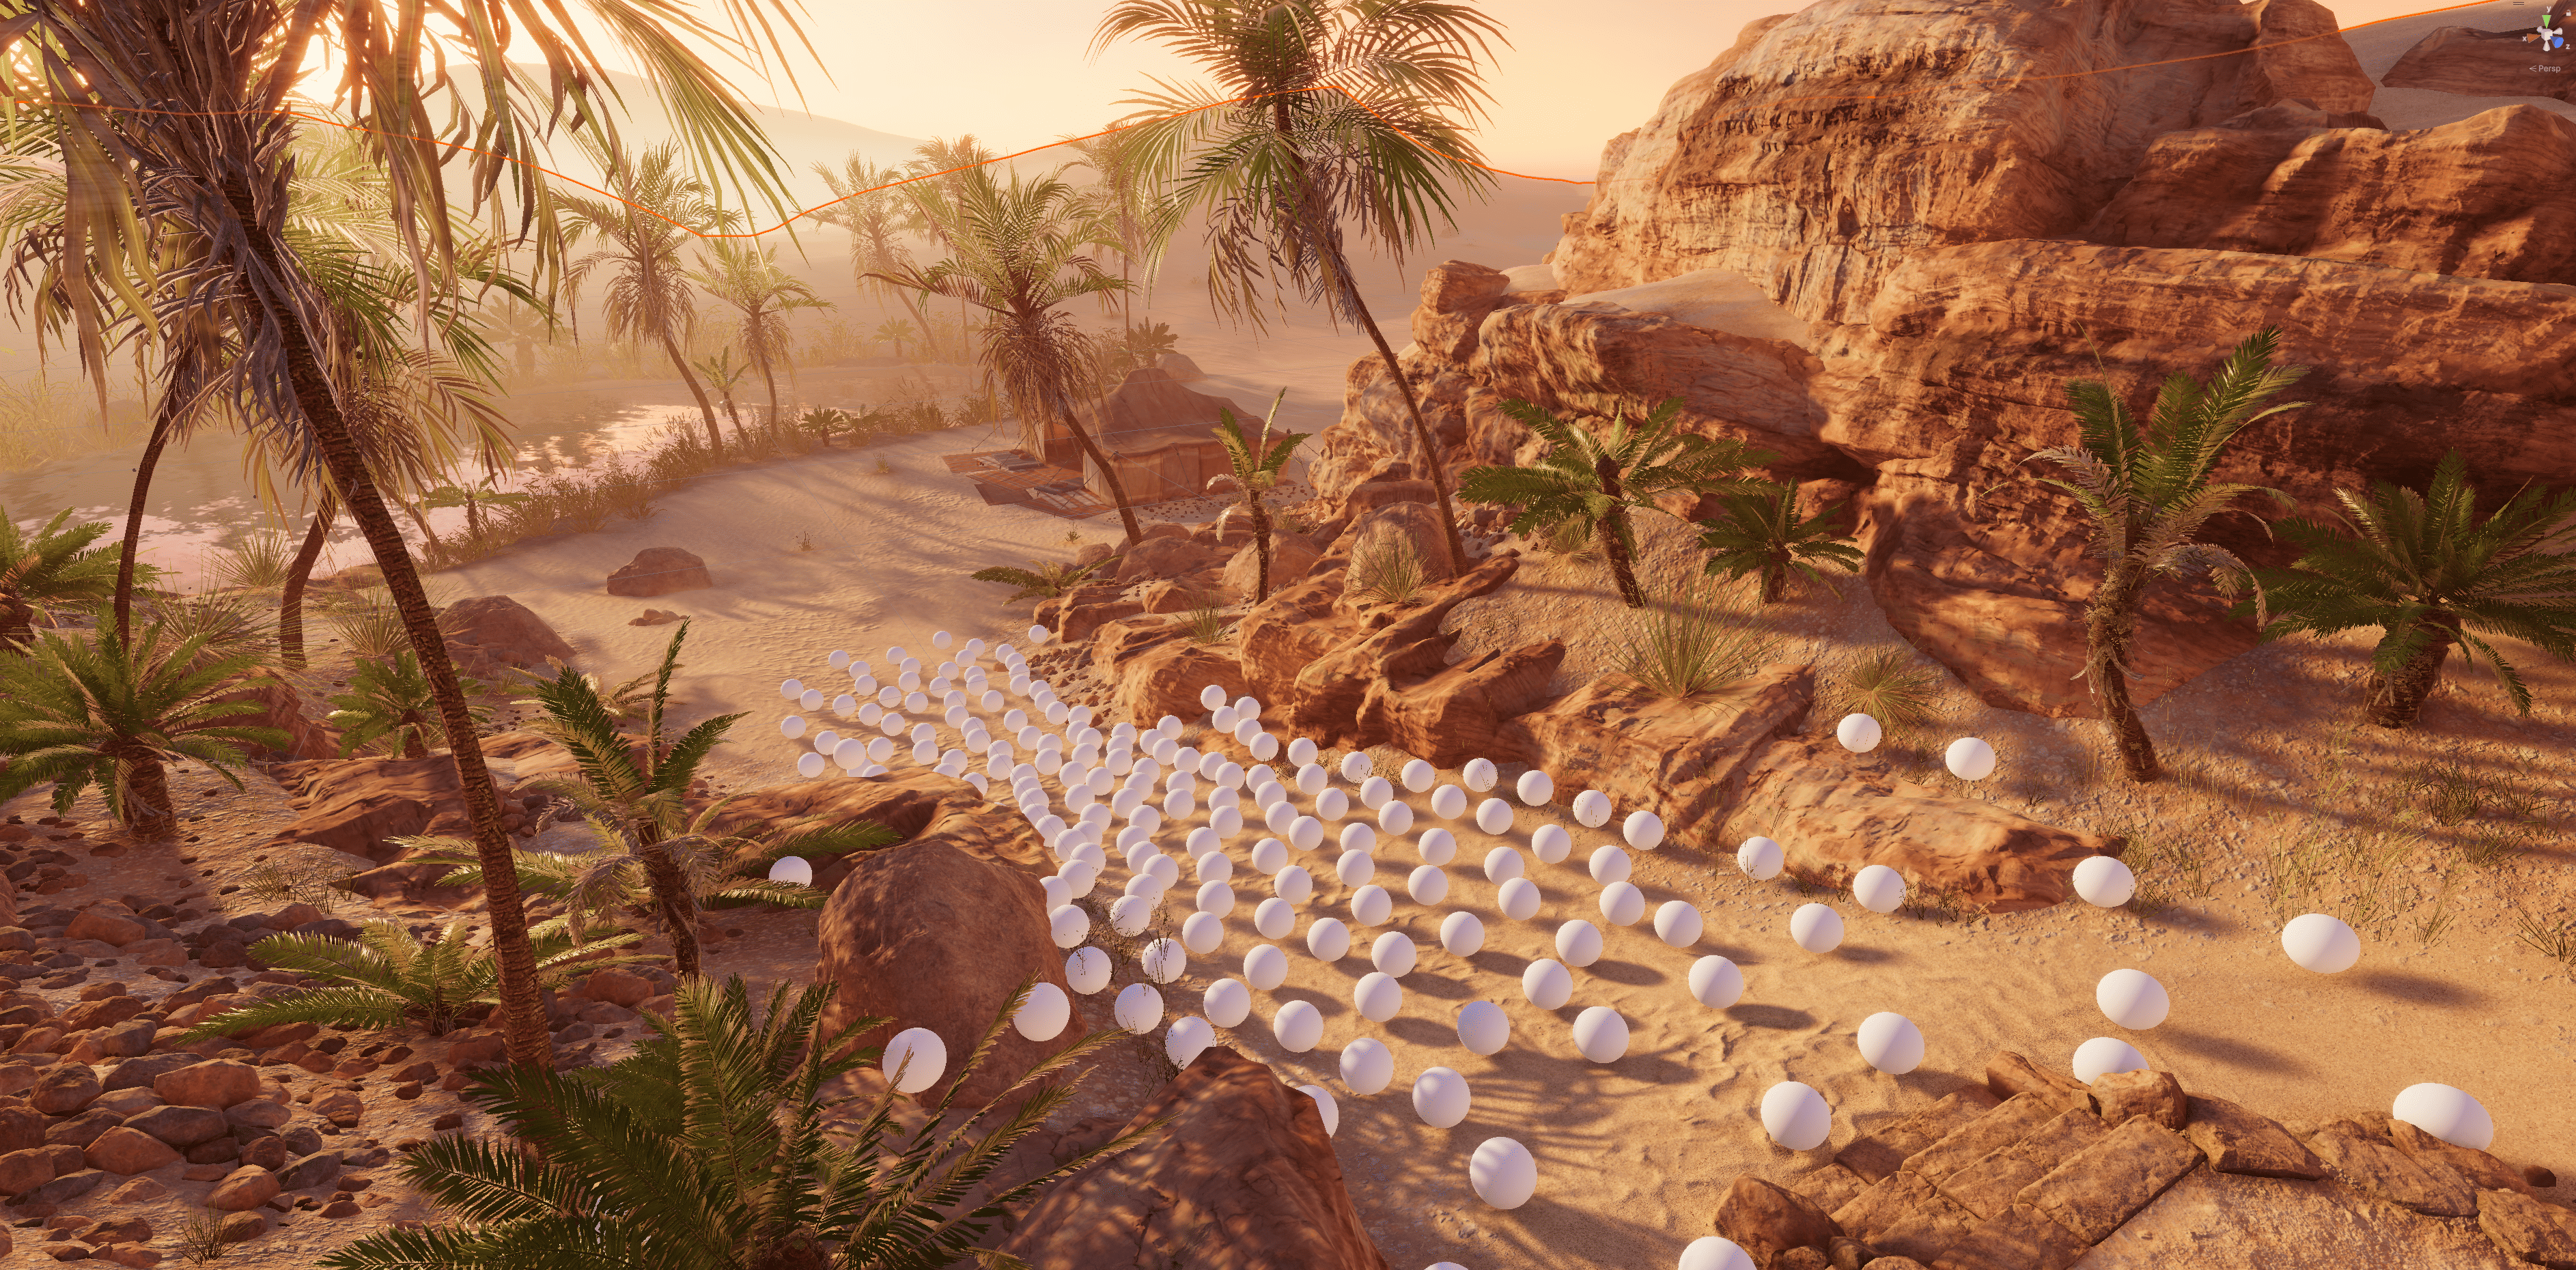
\includegraphics[width=.49\textwidth]{figures/coordination26/oasis/05}
    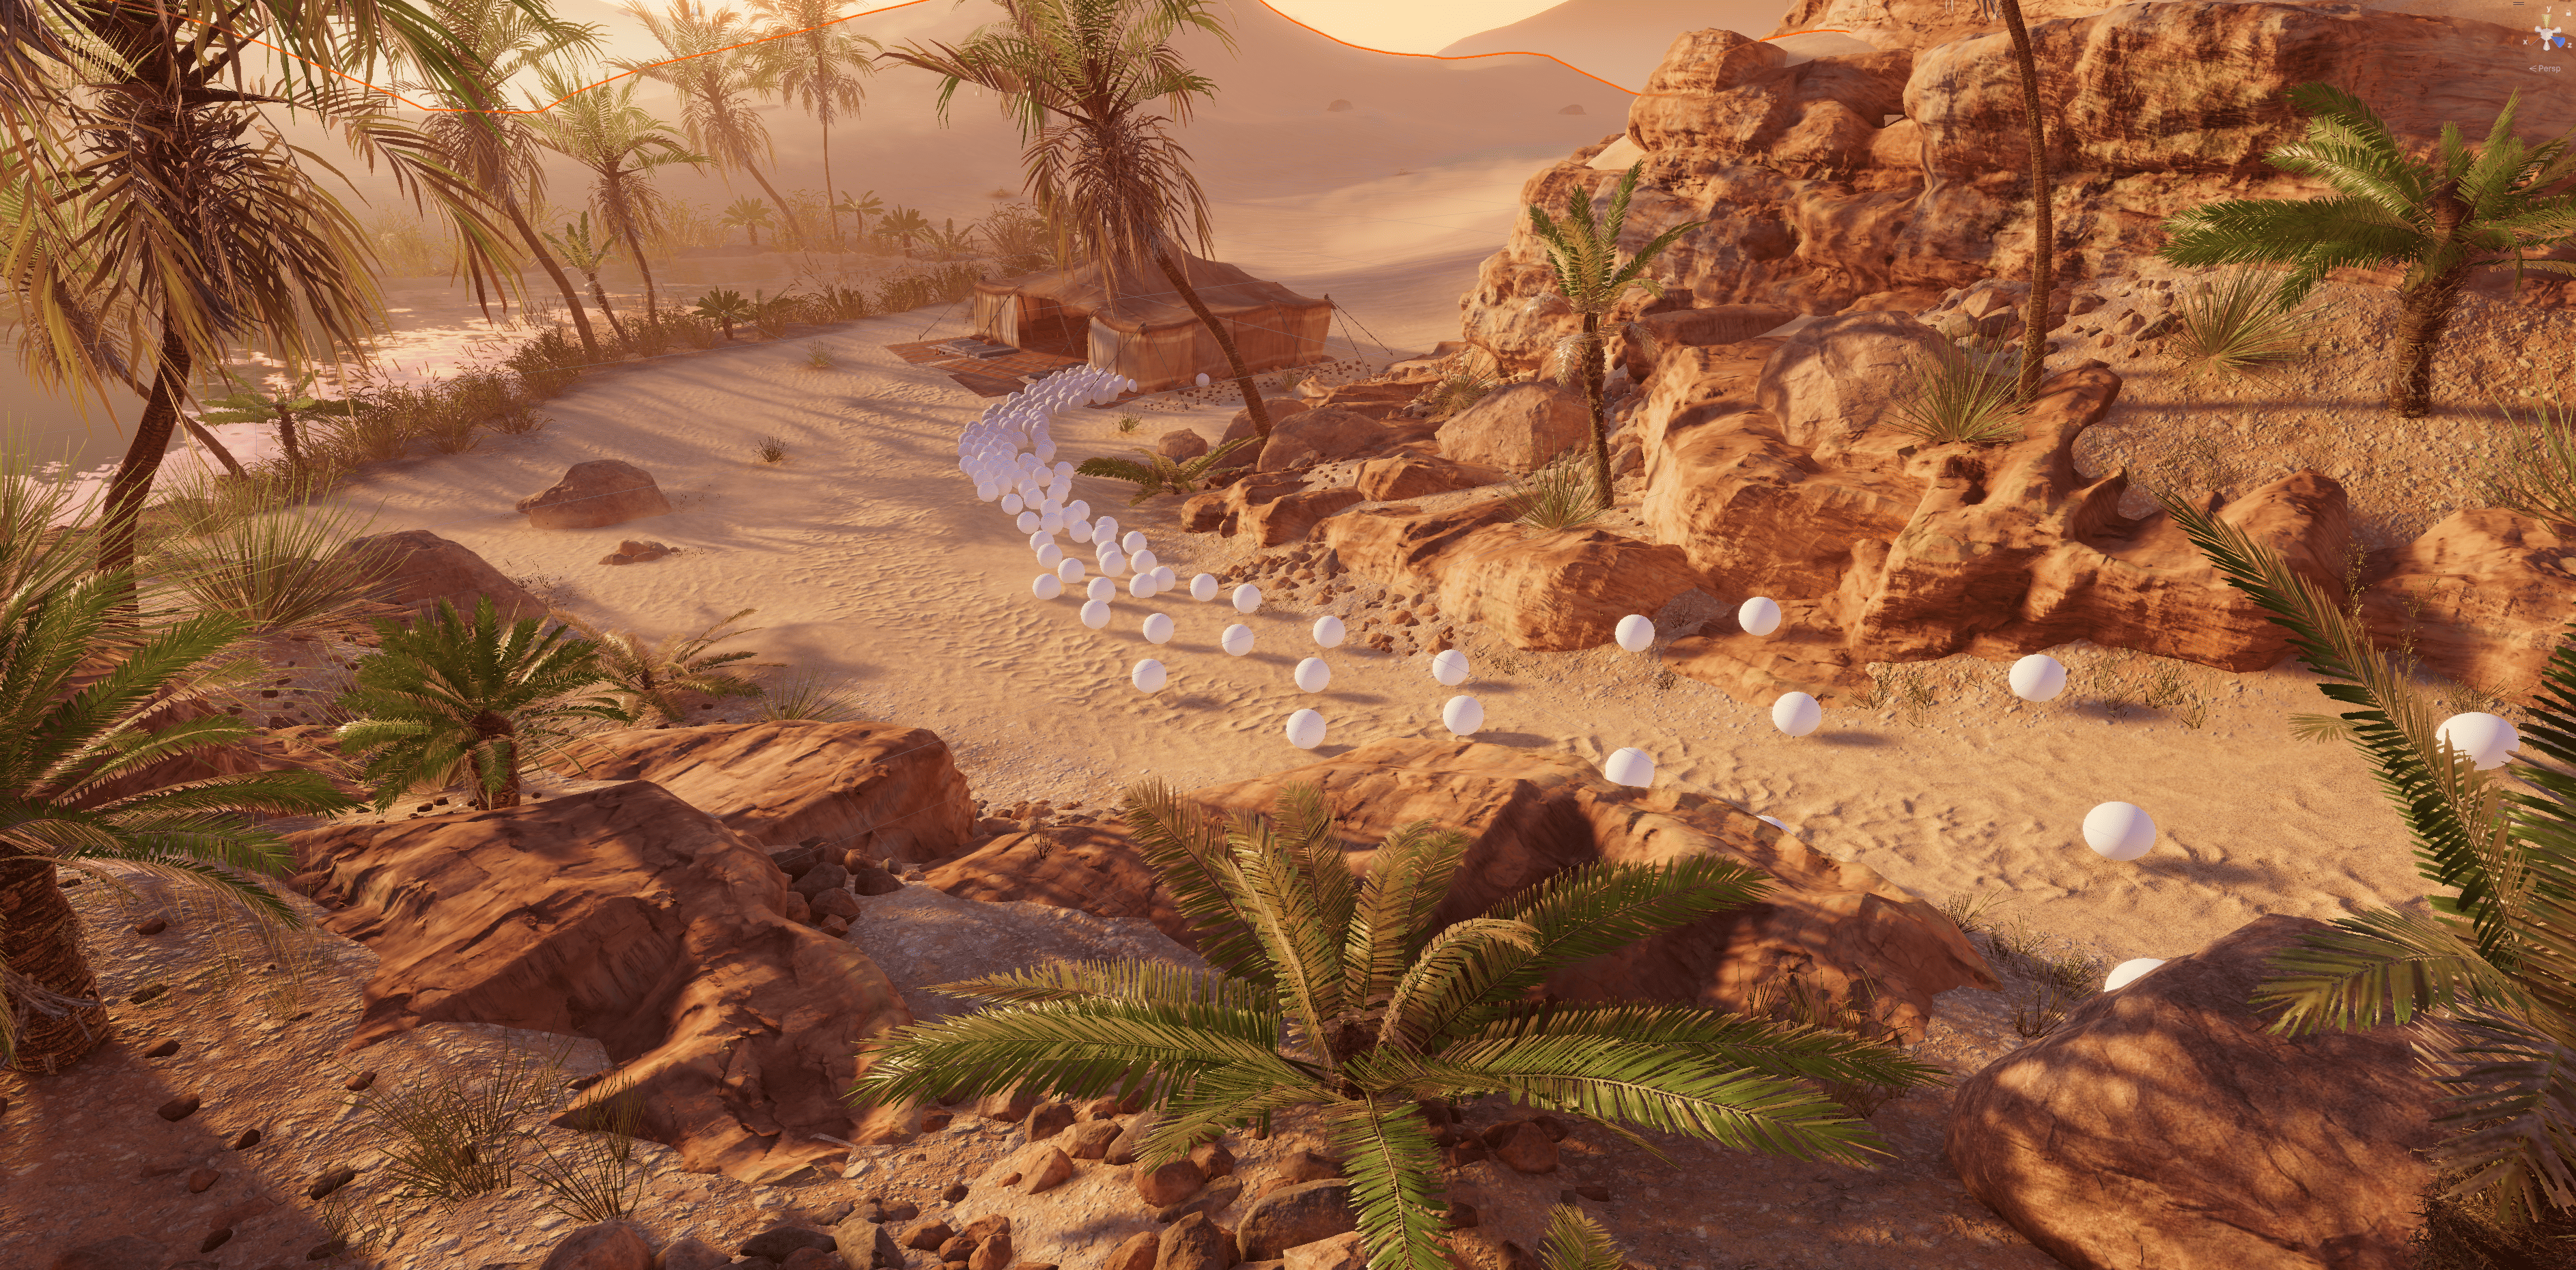
\includegraphics[width=.49\textwidth]{figures/coordination26/oasis/06}
    \caption{Snapshots of the Oasis scenario with 100 nodes.}\
    \label{fig:oasis}
\end{figure}


To showcase the potential of this integration,
we ran the same experiment in one of Unity's built-in environments (i.e., ``Oasis'').
%
In this scenario, obstacles are represented by trees, bushesh, and rocks,
and the source of interest is located inside a tent located on the opposite side of the arena
with respect to the initial placement of the nodes.
%
Snapshots in \Cref{fig:oasis} show the evolution of the system with 100 nodes.
%
This scenario had to be executed on the better equipped desktop to retain real-time performance,
as the increased complexity of the environment
(e.g., more complex geometry, more detailed rendering, and more complex physics interactions)
significantly impacted the performance of the simulation.

\section{Conclusion and Future Work}\label{sec:conclusion}

In this work we presented Collektivity,
a toolchain for the execution of aggregate programs written 
in Collektive on top of the Unity game engine.
%
This integration enables to leverage Unity's physics capabilities 
to create realistic and general-purpose simulations for testing and validating \acp{CAS}.

To achieve this integration,
we designed an architecture to unify the execution model of Unity with the functional nature of aggregate programs,
we extended the Unity engine to support the direct invocation of Collektive computations through \ac{FFI},
while using a shared platform-agnostic data model using Protocol Buffer.
%
To guide the design and implementation of Collektivity, 
we conducted a benchmark to compare the performance of \ac{FFI} and socket-based communication strategies, 
which informed our decision to adopt \ac{FFI} for the integration.
%
Finally, 
we show two examples of unity applications that demonstrates the opportunities of running Collektive on top of Unity,
both of them provided as a starting point for users interested in experimenting with aggregate programming in Unity.

As future work, 
we plan to provide additional example scenarios that showcase more complex aggregate computations,
also including larger populations (e.g., 1{,}000 and 10{,}000 nodes) to demonstrate the scalability of the integration.
%
This will offer users a broader reference set of examples for building their own simulations, 
thereby lowering the entry barrier for experimenting with aggregate programming in Unity.
%
We also plan to compare the current implementation with an \ac{ECS}-based one,
which is a design pattern widely adopted in game development and recently supported by Unity through its \ac{DOTS} framework\footnote{\url{https://unity.com/dots}}.

As discussed in \Cref{subsec:requirements},
the main technical and design challenges encountered in the integration are expected to recur,
at least in part, in other game engines.
%
To assess this hypothesis,
we plan to integrate Collektive with another game engine, such as Unreal Engine or Godot.
%
This would help evaluate the generality of the proposed design and identify which aspects transfer across engines
and which require engine-specific solutions.
